\documentclass[12pt]{report}
\usepackage{fancyhdr}
\usepackage[a4paper, margin=1in]{geometry}
\usepackage{graphicx}
\usepackage{titlesec}
\usepackage{tocloft}
\usepackage{setspace}
\usepackage{caption}
\usepackage{float}
\usepackage{longtable}
\usepackage{amsmath}
\usepackage{amssymb}
\usepackage{enumitem}
\usepackage{array}
\usepackage{tabularx}
\usepackage{needspace}
\usepackage{adjustbox}
\usepackage{multirow}
\usepackage[utf8]{inputenc}

% ----- Fix uneven word spacing -----
\usepackage{microtype}
\sloppy
\emergencystretch=3em

% ----- Remove extra space after punctuation -----
\frenchspacing

\renewcommand{\arraystretch}{1.4}
\setlength{\tabcolsep}{6pt}
\setlength{\parindent}{0pt}
\setlength{\parskip}{6pt}
\onehalfspacing

% Hyperref
\usepackage[
    backref=page,
    colorlinks=true,
    linkcolor=black,
    filecolor=black,
    urlcolor=blue,
    citecolor=blue
]{hyperref}

% Backref Formatting
\renewcommand*{\backref}[1]{}
\renewcommand*{\backrefalt}[4]{%
  \ifcase #1 %
  \or
    (Cited on p.~#2)%
  \else
    (Cited on pp.~#2)%
  \fi
}

\graphicspath{{figures/}}

\begin{document}

% ---------------- Title Page ----------------
\begin{titlepage}
\pagenumbering{roman}
\centering
\vspace*{1cm}

{\LARGE \textbf{KickSense: Intelligent Penalty Kick Analysis Using Pose Estimation}}\\[2cm]


\includegraphics[width=6cm]{BUI-Logo.jpg}\\[2cm]

Ashir Ijaz\\
\textbf{01-135231-017}\\[0.5cm]
Ibrahim Tariq\\
\textbf{01-135231-037}\\[1.5cm]


Supervisor: Ms. Zainab Iftikhar\\[1.5cm]

{\large \textbf{Bachelor of Science in Computer Science}}\\[0.5cm]
Department of Computer Science\\
Bahria University, Islamabad\\[0.5cm]
September 2026


\vfill
\end{titlepage}


% ---------------- TOC ----------------
\tableofcontents
\clearpage
\listoffigures
\clearpage
\listoftables
\cleardoublepage

% ---------------- Acronyms and Abbreviations ----------------
\chapter*{Acronyms and Abbreviations}
\addcontentsline{toc}{chapter}{Acronyms and Abbreviations}

\vspace{1cm}

\begin{tabbing}
\hspace{4cm}\=\hspace{8cm}\=\kill

\textbf{API} \> Application Programming Interface \\
\textbf{BN} \> Batch Normalisation \\
\textbf{CE} \> Categorical Cross Entropy \\
\textbf{CNN} \> Convolutional Neural Network \\
\textbf{Conv1D} \> One Dimensional Convolution \\
\textbf{CV} \> Computer Vision \\
\textbf{FPS} \> Frames Per Second \\
\textbf{FYP} \> Final Year Project \\
\textbf{GUI} \> Graphical User Interface \\
\textbf{HLD} \> High Level Design \\
\textbf{IDE} \> Integrated Development Environment \\
\textbf{JSON} \> JavaScript Object Notation \\
\textbf{LLD} \> Low Level Design \\
\textbf{LSTM} \> Long Short Term Memory \\
\textbf{MAE} \> Mean Absolute Error \\
\textbf{mIoU} \> Mean Intersection over Union \\
\textbf{MSE} \> Mean Squared Error \\
\textbf{RMSE} \> Root Mean Squared Error \\
\textbf{ReLU} \> Rectified Linear Unit \\
\textbf{RGB} \> Red Green Blue \\
\textbf{ST-GCN} \> Spatial Temporal Graph Convolutional Network \\
\textbf{TFLite} \> TensorFlow Lite \\
\textbf{UI} \> User Interface \\
\textbf{VS Code} \> Visual Studio Code \\
\end{tabbing}
\clearpage
\pagenumbering{arabic}

% ================= Chapter Header Setup =================

\pagestyle{fancy}

% Clear all headers/footers
\fancyhf{}

% Remove header rule on all pages by default
\renewcommand{\headrulewidth}{0pt}

% Define custom chapter mark
\renewcommand{\chaptermark}[1]{%
  \markboth{CHAPTER \thechapter\ -- #1}{}}

% Right header (ONLY from page 2 of chapter)
\fancyhead[R]{\leftmark}

% Page number center footer
\fancyfoot[C]{\thepage}

% First page of each chapter (plain style)
\fancypagestyle{plain}{
  \fancyhf{}
  \renewcommand{\headrulewidth}{0pt}
  \fancyfoot[C]{\thepage}
}
% ========================================================


% ---------------- Chapters ----------------
\chapter{Introduction}
A penalty kick is the most isolated and the most decisive event in football. The ball is placed eleven metres from goal, one player takes the kick, one goalkeeper defends a mouth two hundred and forty four centimetres high and seven hundred and thirty two centimetres wide, and the ball reaches the goal line in roughly four tenths of a second. Human reaction time, measured from the visual stimulus to the beginning of a lateral dive, sits between two hundred and three hundred milliseconds for trained goalkeepers, which leaves almost no margin for a decision taken after the ball has been struck. Goalkeepers therefore do not react to the ball at all. They read the kicker, and they commit to a side before contact. Every coaching manual describes the same set of cues, namely the angle of the run up, the orientation of the hips at the moment the plant foot lands, the position of the shoulders, and the swing plane of the kicking leg. KickSense is built on the observation that these cues are precisely the quantities that a modern pose estimation library recovers automatically from ordinary video. If a coach can learn to read a skeleton, a model can be trained to read the same skeleton, and the reading can be made explicit, repeatable and measurable rather than intuitive.

The problem matters beyond the individual save. Penalty shootouts decide knockout football at every level, and the analytical support available to a goalkeeper is still remarkably thin. Professional clubs employ analysts who watch hours of footage manually and assemble dossiers on opposition penalty takers, a process that is expensive, slow and inherently subjective. Below the professional tier the support disappears entirely. A university side, an academy team or a school goalkeeper has no realistic path to a quantified profile of an opponent's penalty technique. The barrier is not the availability of video, because almost every match at every level is now recorded on a phone, but the availability of analysis. KickSense addresses exactly that gap by turning a single short clip, of the kind anyone can record from behind the goal or from the side of the pitch, into a structured prediction: the side the kicker is preparing to shoot towards, the confidence attached to that prediction, and an estimate of how firmly the ball is about to be struck. The system requires no motion capture suit, no calibrated multi camera rig and no wearable sensor, which is the property that makes it deployable in the environments where analytical support is currently absent.

The work completed so far establishes the full analytical chain end to end, and every component of that chain is operational rather than conceptual. A corpus of three hundred and one penalty kick videos was assembled from broadcast tournament footage and from sessions recorded specifically for this project, and two hundred and fifty nine of those clips carry a complete manual annotation covering shot direction, shot power, outcome, ball placement and the kicker's dominant foot. Each clip is decomposed into individual frames, each frame is passed through MediaPipe Pose to recover thirty three body landmarks with a visibility score, and the resulting variable length landmark stream is converted into a fixed size tensor of twenty six time steps by one hundred and thirty two features through hip centred translation, torso height scaling and linear temporal resampling. Two hundred and twenty five of the annotated clips survive the pose quality filters and form the modelling dataset, split into one hundred and fifty seven training, thirty four validation and thirty four test sequences with the class proportions preserved. A multi task network combining one dimensional convolutions with stacked Long Short Term Memory layers consumes these tensors and produces both a three way direction classification and a scalar power regression from a shared representation. The strongest configuration recorded a validation direction accuracy of 55.9 percent, well above the 33.3 percent expected from random guessing on three classes, and the pipeline is exposed through a Streamlit demonstration application that accepts an uploaded clip and returns the prediction with the pose overlay drawn on the video. The benefit of having built the chain in this order is that the expensive and irreversible part of the project, namely the collection and annotation of a bespoke dataset that does not exist publicly, is now complete and reusable. Every subsequent improvement, whether an architectural change, a hyperparameter search or an additional label, operates on the same stored intermediate artefacts and can be evaluated against the same held out split without repeating any of the earlier stages.

The limitations that motivated the project are the same ones that make the current results honest rather than impressive, and it is worth stating them plainly. Existing academic work on penalty prediction is almost entirely built on proprietary or unpublished datasets, which makes reproduction impossible and comparison meaningless. The approaches that report the strongest numbers depend on heavy machinery, typically semantic video segmentation followed by three dimensional convolution over full pixel volumes, which demands substantial computation and cannot run on a phone or on the modest hardware available to a non professional team. Broadcast footage, which is the only large scale source of penalty video, is filmed for entertainment rather than analysis, so camera angles change between clips, the kicker is frequently partially occluded by defenders or by the frame edge, resolution varies, and the moment of contact is often cut away to a crowd reaction. KickSense copes with these constraints deliberately rather than accidentally. Working on skeleton coordinates instead of pixels reduces each frame from hundreds of thousands of values to one hundred and thirty two, which shrinks the model to under a quarter of a million parameters and makes training feasible on a laptop and inference feasible in real time. Hip centred normalisation and torso height scaling remove the camera position and the apparent size of the player from the representation, so a clip filmed from behind the goal and a clip filmed from the touchline become comparable. Temporal resampling to a fixed twenty six steps removes the dependence on frame rate and clip length. An explicit quality gate rejects any clip in which fewer than ten frames or fewer than twenty percent of frames yield a usable pose, which converts the occlusion problem from a source of silent label noise into a measured and reported rejection rate. What remains, and what the remainder of this report does not attempt to hide, is that two hundred and twenty five sequences is a small dataset for a temporal deep learning model, that the class distribution is uneven, that the power annotation is a subjective human judgement rather than a physical measurement, and that the resulting accuracy is meaningfully better than chance but not yet at a level that would be trusted in a competitive setting.

\begin{figure}[H]
    \centering
    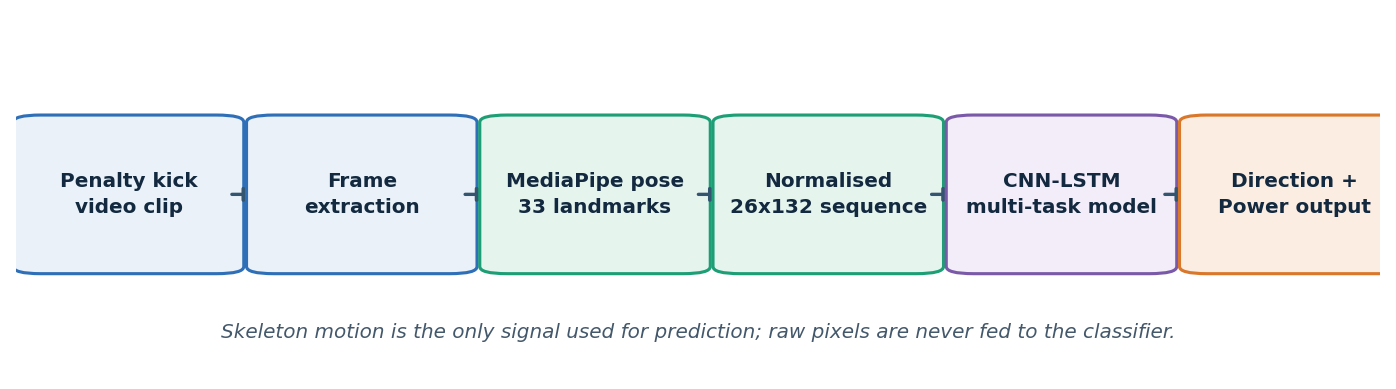
\includegraphics[width=0.99\textwidth]{fig01_concept_overview.png}
    \caption{Conceptual overview of the KickSense processing chain}
    \label{fig:concept}
\end{figure}

\noindent
\textbf{Description:} This figure states the method in its shortest form. A penalty clip is decomposed into frames, each frame is reduced to a thirty three landmark skeleton, the skeleton stream is normalised and resampled into a fixed size tensor, and a multi task network predicts both the shot direction and the shot power from that tensor. The property that defines the approach is that raw pixels never reach the classifier, so the model cannot learn from kit colour, stadium, crowd or broadcast graphics, only from how the kicker moves.

\section{Background}

Football analytics has moved through three broad phases. The first was notational analysis, in which trained observers manually tallied events such as passes, shots and tackles from video, producing reliable but extremely labour intensive data. The second was automated event and trajectory tracking, in which optical systems installed in stadiums recovered the positions of all players and the ball at high frequency, enabling spatial and tactical analysis at scale but requiring infrastructure available only to elite competitions. The third and current phase is the analysis of individual technique, in which the interest shifts from where a player is to how a player moves, and this is the phase in which human pose estimation has become the enabling technology.

Human pose estimation recovers the two dimensional or three dimensional coordinates of anatomical keypoints from an image. The field advanced rapidly after the introduction of convolutional architectures that predict per joint heatmaps, and it became practically deployable when lightweight pipelines began to run at interactive frame rates on commodity hardware. MediaPipe Pose, the library used in this project, follows a two stage detector and tracker design and returns thirty three landmarks per frame, each with a normalised horizontal coordinate, a normalised vertical coordinate, a depth estimate relative to the hip midpoint, and a visibility confidence. The significance for sports analysis is that a video sequence can be reduced to a compact numerical description of body motion, discarding kit colour, pitch texture, crowd background and broadcast graphics while retaining the biomechanical content that actually determines the outcome of a technical action.

The specific biomechanics of penalty kicking have been studied extensively in sports science, and the findings are consistent. The orientation of the pelvis at the instant the support foot is planted is the single strongest predictor of shot direction, because the hips must open towards the target for the leg to swing through the ball on the required line. The angle of the run up approach, the lean of the trunk, the position of the non kicking arm used for balance, and the height and speed of the backlift of the kicking leg all carry additional directional information. Shot power correlates with the angular velocity of the shank at contact, with the length of the backswing, and with the forward momentum generated during the final approach stride. Each of these quantities is, at least in principle, recoverable from the landmark trajectories that MediaPipe produces, which is what makes a pose driven model a natural fit for this task rather than an arbitrary architectural choice.

The remaining background element is the state of publicly available data. There is no standard benchmark dataset for penalty kick direction prediction. General purpose action recognition corpora contain football clips but do not annotate penalty direction or power. Sports specific datasets tend to focus on event spotting, player detection or tracking rather than on the fine grained technique of a single isolated action. This absence is the reason a bespoke corpus had to be collected and annotated for this project, and it is also the reason that a direct numerical comparison against published penalty prediction results cannot be made fairly, a point developed further in Chapter 2 and quantified in Chapter 4.

\section{Objective}

The objective of KickSense is to demonstrate that the directional and power intent of a football penalty kick can be predicted from the kicker's body motion alone, using only ordinary single camera video, at a computational cost low enough for the system to run on consumer hardware. The prediction must be produced before the moment of ball contact is required as input, so that the output is genuinely anticipatory rather than a retrospective description of a completed event, and it must be accompanied by a calibrated confidence value so that a user can distinguish a confident reading from an uncertain one.

Supporting this primary objective is a methodological aim of equal importance to the project, namely that every stage of the pipeline should be reproducible and independently inspectable. Intermediate artefacts are written to disk at every step, so extracted frames, landmark arrays, normalised tensors and the stratified split indices all persist between runs. This makes it possible to change one component, retrain, and attribute the resulting difference in accuracy to that component alone, which is the property that the ablation study reported in Chapter 4 depends on.

\section{Problem Description}

The core problem is a temporal sequence classification problem under severe data scarcity and severe input variability. Given a short video clip of a football penalty kick, the system must assign the clip to one of three directional classes and produce a scalar power estimate, using a training set of a few hundred examples drawn from footage that was never intended for analytical use. Several distinct difficulties combine to make this hard, and each was observed directly during development rather than anticipated from the literature.

\begin{enumerate}[label=\roman*.]
    \item Broadcast penalty footage is filmed from inconsistent camera positions, so the same physical motion produces very different pixel patterns and very different raw landmark coordinates across clips.
    \item The kicker is frequently occluded by the goalkeeper, by teammates in the frame, or by the edge of the frame itself, which causes MediaPipe to fail on a substantial fraction of frames.
    \item Clip lengths and frame rates vary widely, so the number of frames available per kick ranges from a few dozen to several hundred and cannot be assumed constant.
    \item The three directional classes are not balanced, because penalty takers in real matches shoot to the corners far more often than down the middle.
    \item Shot power has no ground truth measurement available from video, so the annotation is a human judgement on a one to ten scale and carries irreducible subjective noise.
    \item The total quantity of labelled data is small relative to the capacity of any temporal deep learning architecture, which makes overfitting the default outcome unless it is actively suppressed.
\end{enumerate}

\section{Project Objectives}

The project was decomposed into a set of concrete, verifiable objectives, each of which maps onto a specific deliverable in the codebase.

The first objective is the construction of an annotated penalty kick corpus, since no suitable public dataset exists. This required sourcing broadcast clips across multiple tournaments, recording additional footage locally to increase the volume and the diversity of camera angles, cutting each source video down to the penalty action itself, and manually annotating shot direction, shot power, outcome, ball placement, dominant foot, match and tournament for every clip in a single spreadsheet that acts as the project's label authority.

The second objective is a reliable pose extraction stage that converts video into landmark sequences and reports its own failure rate honestly. This means running MediaPipe Pose at its highest model complexity over every extracted frame, storing the resulting landmark array per clip, and recording how many frames yielded a detection so that clips with insufficient pose coverage can be identified and excluded rather than silently degrading the training signal.

The third objective is a preprocessing stage that makes clips comparable to one another. Raw landmark coordinates are dominated by where the player happens to stand in the frame and how large the player appears, neither of which carries any information about shot direction. The preprocessing stage removes both effects through hip centred translation and torso height scaling, and removes the effect of variable clip duration through resampling to a fixed number of time steps.

The fourth objective is a multi task predictive model that produces both outputs from a shared representation, on the reasoning that the body motion which determines direction also determines power, so a shared encoder should be more sample efficient than two independent models trained on the same small dataset.

The fifth objective is an honest evaluation protocol. The system must be assessed on a held out test split that is never used for model selection, using accuracy, per class precision, recall and F1 score, a confusion matrix, and regression error metrics for the power head, with the three class random baseline stated explicitly so that any reported accuracy can be interpreted correctly.

The sixth objective is a usable interface. A Streamlit application accepts an uploaded clip, runs the full pipeline, renders the pose overlay so that the user can see what the model actually observed, and displays the direction prediction with its confidence distribution alongside the power estimate. A FastAPI service wraps the same inference path so that the planned mobile and web client can call it over HTTP.

\section{Project Scope}

The scope of the current phase of KickSense covers the complete offline analytical pipeline together with a single user demonstration interface. In scope are dataset collection and annotation, frame extraction, pose estimation, preprocessing and normalisation, model construction, training with augmentation and regularisation, quantitative evaluation on a held out split, ablation analysis of the architectural and training choices, qualitative inspection of pose overlays, and the Streamlit demonstration application together with the FastAPI wrapper that exposes the inference path as a service.

Deliberately outside the scope of this phase are several capabilities that would be natural extensions but that were not attempted, and it is important to be explicit about them rather than imply a completeness the system does not have. The system does not track the ball, so the ball placement annotation present in the label file is recorded but unused by the model. The system does not perform goalkeeper analysis, so it makes no recommendation about where a keeper should dive and no assessment of the keeper's own movement. The system operates on a single kicker per clip and does not handle multi player scenes. It does not run on video streams in real time from a camera feed, only on uploaded files. It produces no three dimensional reconstruction of the kick, since the depth value returned by MediaPipe is a relative estimate rather than a calibrated measurement and was not found to be reliable enough to build on. Finally, the mobile client is designed but not implemented, which is why it appears in the future work of Chapter 5 rather than in the results of Chapter 4.

\section{Solution Application Areas}

The most direct application is goalkeeper preparation. A goalkeeper or goalkeeping coach can assemble clips of an opponent's previous penalties and obtain a quantified profile of that player's directional tendencies together with the confidence of each reading, which converts an informal impression into something that can be reviewed, argued with and updated as new footage arrives.

A second application is technique coaching for the kicker rather than the keeper. If a model can identify the side a kicker is aiming for from the body motion alone, then that kicker's motion is leaking their intention, and the specific landmark trajectories that drove the prediction indicate where the leak is. A player whose direction is predicted with high confidence from the hip orientation at plant foot contact has a concrete, actionable technical flaw to work on.

A third application is academic and pedagogical. The pipeline is a compact, fully documented example of skeleton based temporal action analysis on a real and difficult dataset, and the intermediate artefacts at every stage make it suitable as a teaching resource for computer vision and sequence modelling. The honest reporting of the failure modes, in particular the pose detection failure rate on broadcast footage and the impact of a small unbalanced dataset, is arguably more instructive than a polished result would be.

A fourth application area, contingent on the mobile client planned in Chapter 5, is grassroots and academy use. The defining property of the system is that it requires only a phone camera and no installed infrastructure, so the analytical support currently confined to professional clubs becomes accessible to teams that have video but no analysts.

\begin{figure}[H]
    \centering
    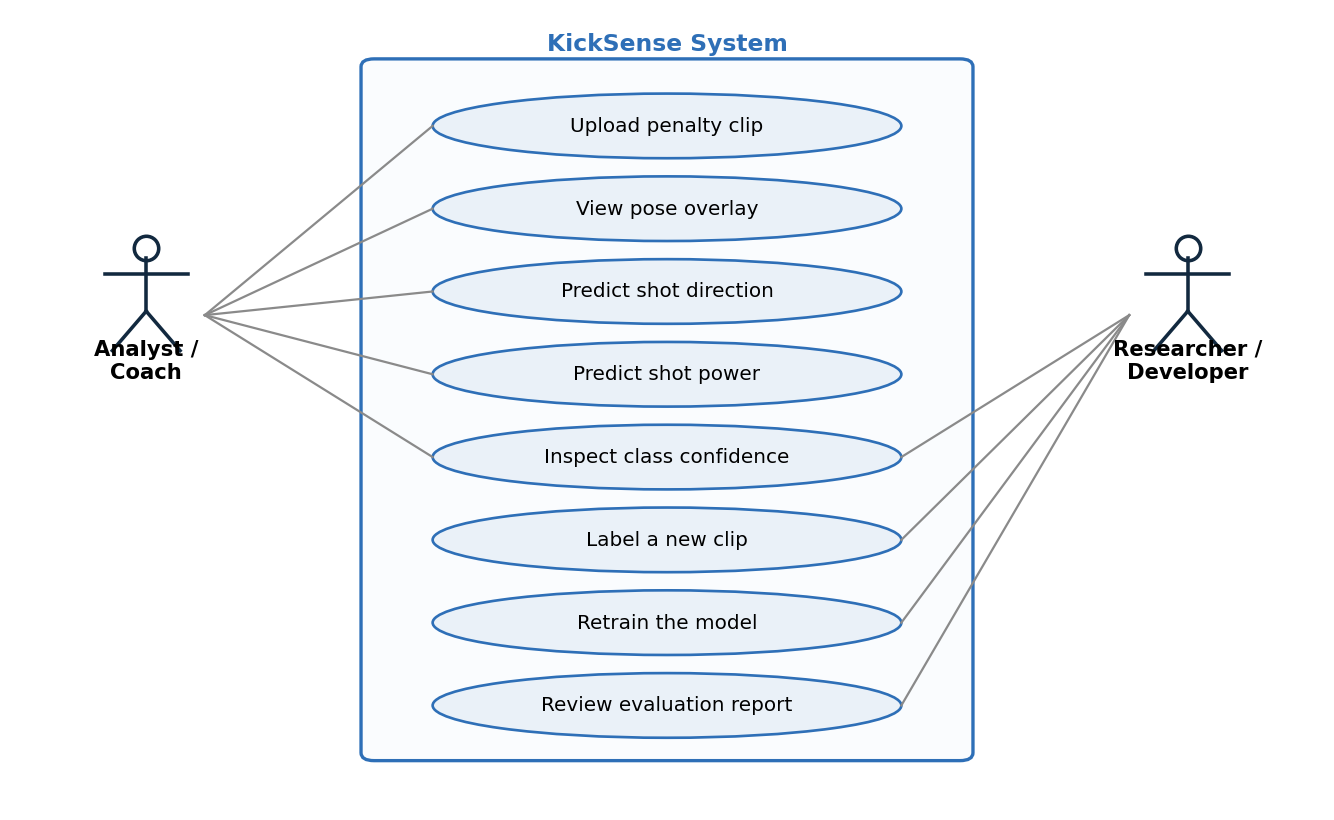
\includegraphics[width=0.95\textwidth]{fig03_usecase_diagram.png}
    \caption{Use case diagram of the KickSense system}
    \label{fig:usecase}
\end{figure}

\noindent
\textbf{Description:} This diagram identifies the two actors the system serves and the operations available to each. The analyst or coach uploads a penalty clip, inspects the rendered pose overlay to confirm the system observed the player correctly, and reads the direction and power predictions together with the class confidence distribution. The researcher or developer additionally annotates new clips, retrains the model on the expanded corpus, and reviews the evaluation report. Inspecting class confidence is available to both actors, because a prediction accompanied by a low confidence value should be treated differently from a confident one by anyone reading it.

\section{Risk Involved}

\subsection{Data Scarcity and Class Imbalance}

The most significant risk to the project is the size of the dataset. Two hundred and twenty five usable sequences is small for a model containing roughly a quarter of a million parameters, and the direction classes are unbalanced with one hundred and seven left, ninety four right and fifty eight centre examples. The consequences are visible in the results, since the model overfits the training set rapidly and the centre class is recognised least reliably. The risk is mitigated but not eliminated by a fivefold augmentation strategy, by aggressive dropout and batch normalisation, by early stopping on validation accuracy, and by a stratified split that guarantees every class appears in every partition. The residual risk is managed by continuing to record additional footage, with the locally recorded sessions already contributing sixty one clips to the corpus.

\subsection{Pose Estimation Failure on Broadcast Footage}

The pipeline is entirely dependent on MediaPipe recovering a usable skeleton, and on broadcast footage this frequently fails because the kicker is occluded, small in frame, or motion blurred. If failures were allowed through silently they would inject sequences of interpolated or duplicated frames into the training data and corrupt the learned representation. The mitigation is the explicit quality gate described in Chapter 3, which rejects clips falling below a minimum absolute frame count and a minimum detection ratio, and which converts a hidden data quality problem into a reported and quantified rejection rate. The cost of this mitigation is a smaller dataset, which feeds directly back into the first risk.

\subsection{Label Subjectivity in the Power Annotation}

Shot direction is objectively verifiable from the footage, but shot power was annotated by human judgement on a one to ten scale with no instrumented ground truth. The distribution of these labels is heavily concentrated, with a large cluster at the maximum value, which suggests that the annotation compresses a continuous physical quantity into a coarse and inconsistently applied ordinal scale. The regression head therefore learns a target that is itself noisy, and its reported error should be read as an upper bound on achievable accuracy rather than as a measure of the model's capability. The mitigation applied is to weight the power loss at 0.3 relative to the direction loss so that noisy power targets cannot dominate the shared representation, and the planned mitigation is to replace the subjective scale with a measurement derived from ball displacement between consecutive frames.

\subsection{Configuration Drift Between Training and Inference}

A practical engineering risk identified during development is that the preprocessing applied at inference time must match the preprocessing applied at training time exactly, since any discrepancy silently degrades accuracy without producing an error. One such discrepancy was found in the pose estimation configuration, where the training pipeline and the interactive application did not use identical settings. The mitigation is that all preprocessing constants are defined in a single module which both paths import, and that the correction of the remaining configuration mismatch is listed as an explicit item in the future work of Chapter 5.

\clearpage


\chapter{Literature Review}
This chapter surveys the work that KickSense builds on. The review is organised from the outside in, beginning with what sports science has established about how goalkeepers actually anticipate penalties, moving through the pose estimation and skeleton based action recognition machinery that makes automated anticipation possible, and closing on the single most directly comparable publication, namely the penalty prediction model of Salazar and Alatrista-Salas \cite{salazar2024}. That paper is the base work for this project and is treated in detail. The chapter ends with two tables, the first summarising the surveyed literature in the conventional comparative format and the second setting KickSense side by side with the base paper across models, datasets, techniques, limitations and future work.

\begin{figure}[H]
    \centering
    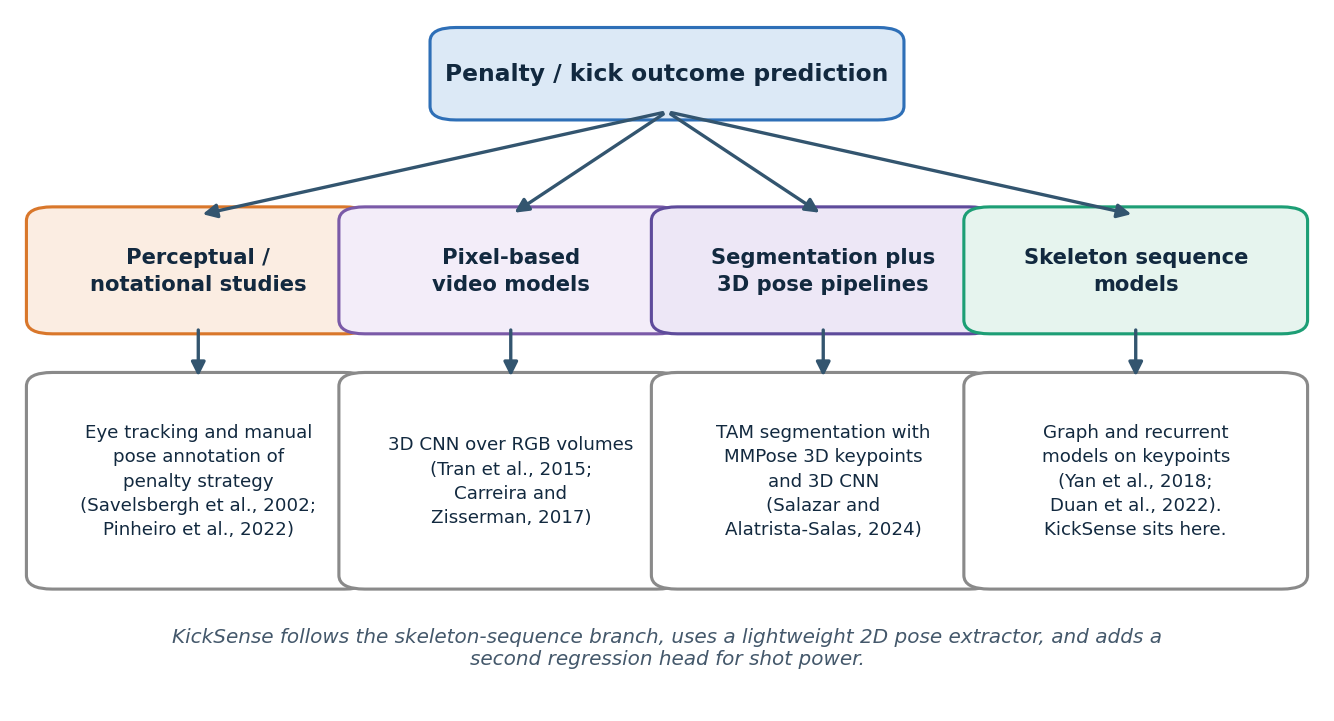
\includegraphics[width=0.98\textwidth]{fig02_research_taxonomy.png}
    \caption{Taxonomy of approaches to penalty and kick outcome prediction}
    \label{fig:taxonomy}
\end{figure}

\noindent
\textbf{Description:} This taxonomy positions KickSense within the existing literature. The leftmost branch covers perceptual and notational studies that established which body cues carry directional information but which rely on human observers. The middle branches cover automated approaches that operate on pixels, either directly through three dimensional convolution or through a segmentation stage followed by three dimensional pose recovery. The rightmost branch covers skeleton sequence models, which is where KickSense sits, using a lightweight two dimensional pose extractor and adding a regression head for shot power that none of the surveyed works provide.

\section{Perceptual Foundations of Penalty Anticipation}

The premise that a penalty kick can be predicted before ball contact is not an assumption of this project but an established experimental finding. Savelsbergh, Williams, van der Kamp and Ward studied expert and novice goalkeepers responding to filmed penalty kicks with a joystick while their eye movements were recorded \cite{savelsbergh2002}. Expert goalkeepers predicted the direction of the kick more accurately, initiated their response later, and made fewer corrective movements, which indicates that they were extracting reliable information from the kicker's body rather than guessing early and adjusting. The eye tracking data localises that information precisely. Novices spent longer fixating the trunk, arms and hips, whereas experts concentrated on the kicking leg, the non kicking leg and the ball region, particularly in the moments immediately before foot to ball contact.

This result is directly load bearing for KickSense in two ways. First, it confirms that the predictive signal exists in the kinematics of the lower body and is available before contact, which is what justifies building a model that consumes only skeletal motion. Second, it identifies which landmarks should matter most, and this expectation is consistent with the finding of the base paper that the legs are the most influential body part for the prediction task \cite{salazar2024}. The limitation of this line of work, from an engineering perspective, is that it measures human perceptual expertise rather than producing an automated system. It tells us the task is solvable and where to look, but it provides no model, no dataset and no reproducible computational pipeline.

Pinheiro, Jin, da Costa and Lames took a step towards automation by integrating body pose estimation with traditional notational analysis to study penalty kick strategy in elite football \cite{pinheiro2022}. Their contribution is methodological: they demonstrate that pose derived measurements can be combined with event annotation to characterise how elite players approach the penalty spot, and they establish that pose estimation output is meaningful at the level of detail required for penalty analysis. The work remains descriptive rather than predictive, in that it quantifies and compares strategies retrospectively without constructing a model that anticipates the direction of an unseen kick, and the analysis pipeline still requires substantial expert involvement rather than running automatically over arbitrary footage.

\section{Human Pose Estimation}

The technical enabler for all automated approaches in this area is human pose estimation, the recovery of anatomical keypoint coordinates from images. The field was reshaped by OpenPose, presented by Cao, Hidalgo, Simon, Wei and Sheikh, which introduced a bottom up architecture using part affinity fields to associate detected body parts into complete skeletons, enabling real time multi person pose estimation for the first time \cite{cao2019}. OpenPose established the practical viability of pose driven video analysis but is computationally demanding, typically requiring a dedicated graphics processor for interactive performance.

Sun, Xiao, Liu and Wang subsequently introduced the High Resolution Network, which maintains high resolution feature representations throughout the network rather than recovering them from low resolution encodings, and which set a new accuracy standard on standard keypoint benchmarks \cite{sun2019}. The accuracy improvement comes with a further increase in computational cost, which places it outside the constraint set of a project intended to run on consumer hardware.

The pose estimator adopted in KickSense is MediaPipe Pose, built on the BlazePose architecture of Bazarevsky and colleagues \cite{bazarevsky2020}, delivered through the MediaPipe perception framework of Lugaresi and colleagues \cite{lugaresi2019}. BlazePose is designed explicitly for on device real time inference and uses a detector followed by a tracker, where the detector localises the person and the tracker regresses thirty three landmarks. The thirty three landmark topology is a deliberate superset of the seventeen keypoint convention used by common benchmarks, adding hands, feet and facial points, and each landmark is returned with a normalised horizontal coordinate, a normalised vertical coordinate, a depth estimate relative to the hip midpoint, and a visibility confidence. The relevant trade off is explicit. MediaPipe is less accurate than the heaviest available estimators and its depth estimate is a relative regression rather than a metric measurement, but it runs at interactive rates on a laptop central processing unit and requires no specialised hardware, which is precisely the property that makes the KickSense deployment target realistic. The limitation observed in practice, and quantified in Chapter 4, is that MediaPipe degrades sharply when the subject is occluded, small in frame or motion blurred, all of which occur routinely in broadcast penalty footage.

\section{Skeleton Based Action Recognition}

Once a video has been reduced to a sequence of skeletons, the classification problem becomes one of temporal sequence modelling over structured coordinates. Two families of approach dominate the literature.

The first family treats the skeleton as a graph. Yan, Xiong and Lin introduced Spatial Temporal Graph Convolutional Networks, which apply graph convolution over the natural connectivity of the human body in the spatial dimension and over time in the temporal dimension \cite{yan2018}. This encodes the anatomical structure of the skeleton directly into the architecture rather than requiring the network to learn it, and it substantially outperformed earlier recurrent baselines on large action recognition benchmarks. Shi, Zhang, Cheng and Lu extended the idea with an adaptive graph whose topology is learned rather than fixed, together with a second stream operating on bone vectors rather than joint positions \cite{shi2019}. Duan, Zhao, Chen, Lin and Dai later revisited the problem and showed that stacking pose heatmaps into a three dimensional volume and applying a three dimensional convolutional network is more robust than graph convolution on joint coordinates, particularly when the pose estimates are noisy \cite{duan2022}.

The second family treats the flattened skeleton as an ordinary multivariate time series and models it with recurrent or convolutional sequence architectures. The Long Short Term Memory unit of Hochreiter and Schmidhuber remains the standard recurrent building block because its gating mechanism allows gradients to propagate over long sequences without vanishing \cite{hochreiter1997}. A common and effective hybrid, and the one adopted by KickSense, places one dimensional convolutions before the recurrent layers so that the convolutions extract short range local motion patterns across neighbouring frames while the recurrent layers integrate those patterns over the whole sequence.

The choice of the recurrent hybrid over the graph based family in this project is driven by dataset size rather than by any claim of superiority. Graph convolutional and heatmap volume approaches were validated on benchmarks containing tens of thousands of labelled sequences. With two hundred and twenty five sequences available, a model with a quarter of a million parameters already overfits, and the additional capacity of a graph network would make that worse rather than better. Evaluating a spatial temporal graph network on this task once the corpus is substantially larger is therefore listed in the future work of Chapter 5.

\section{Video Level Action Recognition}

For completeness it is worth recording the pixel based alternative, since the base paper follows it. Tran, Bourdev, Fergus, Torresani and Paluri demonstrated that three dimensional convolutional networks learn effective spatiotemporal features directly from raw video volumes \cite{tran2015}. Simonyan and Zisserman proposed a two stream design in which one branch consumes appearance and a second consumes optical flow, showing that explicit motion representation is valuable \cite{simonyan2014}. Carreira and Zisserman then introduced the Inflated three dimensional network, which converts a strong two dimensional image classifier into a three dimensional video model by inflating its filters and initialising them from image pretrained weights, which remains a standard baseline for video classification \cite{carreira2017}. Wang and colleagues addressed the sampling problem with Temporal Segment Networks, which sample sparsely across the whole clip rather than densely over a short window \cite{wang2016}.

The strength of this family is that it discards nothing, since colour, texture, ball position and context all remain available to the network. The weaknesses matter a great deal at the scale of a final year project. These models contain tens of millions of parameters, require large pretraining corpora to be effective, and consume video volumes of hundreds of thousands of values per frame, all of which is difficult to justify when the labelled dataset contains a few hundred clips. They are also sensitive to nuisance variation such as camera angle, stadium, kit colour and lighting, none of which carries information about shot direction, and with a small dataset a high capacity pixel model will readily latch onto exactly those spurious correlations.

\section{Football Specific Datasets and Tooling}

The absence of a suitable public dataset is a defining constraint of this project, so it is worth being specific about what does exist. Giancola, Amine, Dghaily and Ghanem released SoccerNet, a large scale dataset for action spotting in broadcast football video, later substantially extended by Deliège and colleagues as SoccerNet version two with a far richer action vocabulary and additional tasks \cite{giancola2018,deliege2021}. These resources are valuable and widely used, but their annotation granularity is the event level, marking that a penalty occurred at a given timestamp, and they do not annotate the direction the penalty was aimed towards or the power with which it was struck. Pappalardo and colleagues published a large public collection of spatiotemporal match event data covering multiple competitions, which is again event level and contains no video or pose information \cite{pappalardo2019}.

The consequence is unavoidable. A model that predicts penalty direction from body motion requires per clip direction labels, and no public dataset provides them. Both the base paper and this project therefore had to construct a bespoke corpus, and since neither corpus is the same as the other, any numerical comparison between them measures the difficulty of two different datasets as much as it measures the quality of two different models. This point governs the way results are compared in Chapter 4.

On the tooling side, the base paper relies on Track Anything for its segmentation stage, an interactive video object segmentation and tracking system built on the Segment Anything foundation model \cite{yang2023,kirillov2023}, and on MMPose for three dimensional pose recovery \cite{mmpose2020}. KickSense is implemented with TensorFlow and Keras for modelling \cite{abadi2016} and scikit-learn for splitting, class weighting and metric computation \cite{pedregosa2011}, with optimisation by Adam \cite{kingma2015} and regularisation by dropout and batch normalisation \cite{srivastava2014,ioffe2015}.

\section{The Base Paper in Detail}

Salazar and Alatrista-Salas present the work most directly comparable to KickSense, published at the ninth International Conference on Machine Learning Technologies in Oslo in 2024 \cite{salazar2024}. Their objective is the same as ours, namely to predict the region of the goal towards which a penalty will be directed from the pose of the kicker, and their framing of the problem as a three way regional classification is the framing this project adopted.

Their methodology proceeds in three stages. They first construct a corpus of penalty kick videos, since no public equivalent exists. They then combine semantic video segmentation using Track Anything with three dimensional pose estimation using MMPose, the purpose of the segmentation stage being to isolate the kicker from the background and from other players so that the pose estimator operates on a clean subject. They finally compare three deep learning models for the prediction task and conduct an analysis of which part of the player's body most affects the prediction, concluding that the legs are the most influential region.

The strengths of the approach are real. The segmentation stage directly attacks the occlusion and clutter problem that degrades pose estimation on broadcast footage, and it does so more thoroughly than a quality filter can, because it improves the input rather than discarding bad cases. Three dimensional pose recovery captures depth relationships, in particular the rotation of the pelvis away from the image plane, that a two dimensional projection can only represent indirectly. Comparing three model families rather than presenting one is methodologically sound, and the body part influence study is exactly the kind of interpretability analysis that makes a result useful to a coach rather than merely accurate.

The limitations are equally real and shaped the design of this project. The pipeline is heavy, since interactive segmentation followed by three dimensional pose estimation followed by three dimensional convolution is far beyond what runs on a phone or on a laptop without a graphics processor, which forecloses the grassroots deployment that motivates KickSense. The corpus is bespoke and not publicly released, so the reported accuracy cannot be independently reproduced and cannot serve as a benchmark. The prediction is restricted to the goal region and does not include any estimate of shot power, so a goalkeeper receives no information about how firmly the ball will be struck. The segmentation stage as described requires human interaction to specify the object to be tracked, which limits the degree to which the pipeline can be applied automatically at scale.

KickSense responds to each of these limitations with a specific design decision rather than a general aspiration. In place of segmentation followed by three dimensional pose estimation, it applies a lightweight two dimensional pose estimator with an explicit quality gate, which removes the human in the loop and reduces the computational cost by orders of magnitude at the price of a measured rejection rate. In place of a single classification head it uses a multi task head that predicts direction and power from a shared representation. In place of an unpublished corpus it maintains a fully documented annotation file, per clip intermediate artefacts and a fixed stratified split, so that every number in this report can be regenerated from the repository. What KickSense does not claim is superiority, since the datasets differ and the comparison would be meaningless, and this is stated explicitly in the summary table and revisited in Chapter 4.

\section{Comparison of Surveyed Literature}

\renewcommand{\arraystretch}{1.3}
\setlength{\tabcolsep}{4pt}
\small

\begin{longtable}{|c|c|>{\raggedright\arraybackslash}p{2.5cm}|
>{\raggedright\arraybackslash}p{2.9cm}|
>{\raggedright\arraybackslash}p{3.0cm}|
>{\raggedright\arraybackslash}p{3.0cm}|}

\hline
\textbf{Ref} & \textbf{Year} & \textbf{Author(s)} &
\textbf{Approach} & \textbf{Contribution} & \textbf{Limitation} \\
\hline
\endfirsthead

\hline
\textbf{Ref} & \textbf{Year} & \textbf{Author(s)} &
\textbf{Approach} & \textbf{Contribution} & \textbf{Limitation} \\
\hline
\endhead

\hline
\multicolumn{6}{r}{\textit{Continued on next page}} \\
\hline
\endfoot

\hline
\endlastfoot

\cite{savelsbergh2002} & 2002 & Savelsbergh et al. &
Eye tracking of expert and novice goalkeepers responding to filmed penalties &
Proves directional information is available before contact and localises it to the kicking and non kicking leg &
Measures human perception only; provides no automated model, dataset or pipeline \\ \hline

\cite{pinheiro2022} & 2022 & Pinheiro et al. &
Body pose estimation combined with notational analysis of elite penalties &
Shows pose measurements are meaningful at the granularity penalty analysis requires &
Descriptive rather than predictive; needs substantial expert involvement per clip \\ \hline

\cite{cao2019} & 2019 & Cao et al. &
Bottom up multi person pose estimation using part affinity fields (OpenPose) &
Made real time multi person pose estimation practical and widely reusable &
Computationally heavy; typically needs a dedicated graphics processor \\ \hline

\cite{sun2019} & 2019 & Sun et al. &
High resolution representation learning for keypoint detection (HRNet) &
Set a new accuracy standard on standard keypoint benchmarks &
Cost rises further; unsuited to on device or laptop only deployment \\ \hline

\cite{bazarevsky2020} & 2020 & Bazarevsky et al. &
Detector plus tracker regression of 33 landmarks for on device use (BlazePose) &
Interactive rate pose estimation on commodity hardware, adopted by this project &
Lower accuracy than heavy estimators; depth is relative, and it fails under occlusion \\ \hline

\cite{yan2018} & 2018 & Yan et al. &
Spatial temporal graph convolution over skeleton joints (ST-GCN) &
Encodes body connectivity into the architecture and beat recurrent baselines &
Validated on tens of thousands of sequences; overfits small corpora \\ \hline

\cite{shi2019} & 2019 & Shi et al. &
Adaptive graph topology with an additional bone vector stream &
Learned topology and second stream improve skeleton action accuracy &
Higher capacity and more hyperparameters, worsening small data overfitting \\ \hline

\cite{duan2022} & 2022 & Duan et al. &
Stacked pose heatmap volumes processed by a 3D CNN (PoseC3D) &
More robust than joint coordinate graphs when pose estimates are noisy &
Reintroduces the memory and compute cost of 3D convolution \\ \hline

\cite{tran2015} & 2015 & Tran et al. &
3D convolution learned directly on raw RGB video volumes (C3D) &
Established spatiotemporal feature learning from pixels &
Tens of millions of parameters; needs large pretraining corpora \\ \hline

\cite{simonyan2014} & 2014 & Simonyan and Zisserman &
Two stream network combining appearance and optical flow &
Showed explicit motion representation materially improves accuracy &
Optical flow computation is expensive and adds a preprocessing dependency \\ \hline

\cite{carreira2017} & 2017 & Carreira and Zisserman &
Filters of a 2D image classifier inflated into 3D (I3D) &
Strong transferable video baseline through image pretraining &
Large model; sensitive to nuisance variation such as camera angle and kit \\ \hline

\cite{hochreiter1997} & 1997 & Hochreiter and Schmidhuber &
Gated recurrent unit for long range sequence modelling (LSTM) &
Enables gradient flow over long sequences, the backbone used here &
Sequential computation limits parallelism relative to newer architectures \\ \hline

\cite{giancola2018} & 2018 & Giancola et al. &
Large scale action spotting dataset for broadcast football (SoccerNet) &
Provides scale and a standard protocol for football video research &
Event level labels only; no penalty direction, power or pose annotation \\ \hline

\cite{deliege2021} & 2021 & Deliège et al. &
Extended action vocabulary and additional tasks (SoccerNet-v2) &
Richer annotation and more football video tasks &
Still event level; cannot supervise direction prediction \\ \hline

\cite{pappalardo2019} & 2019 & Pappalardo et al. &
Public spatiotemporal match event dataset across competitions &
Large reusable public football event resource &
No video and no pose data, so unusable for this task \\ \hline

\cite{yang2023} & 2023 & Yang et al. &
Interactive video object segmentation and tracking (Track Anything) &
High quality subject isolation in video, used by the base paper &
Requires human interaction to initialise the tracked object \\ \hline

\cite{salazar2024} & 2024 & Salazar and Alatrista-Salas &
TAM segmentation with MMPose 3D pose, three deep models compared, body part influence study &
Closest prior work; identifies the legs as the most influential region &
Heavy pipeline, unpublished corpus, no power estimate, human in the loop segmentation \\ \hline

\caption{Summary of the surveyed literature on pose estimation, skeleton action recognition and penalty prediction}
\label{tab:literature-summary}
\end{longtable}
\normalsize
\clearpage

\section{Comparison of KickSense with the Base Paper}

Table \ref{tab:basepaper-compare} sets the base paper and KickSense against each other across the dimensions that matter for this project. The final row is the most important one, because it states what each work leaves undone and therefore what the remaining phase of this project is committed to delivering.

\renewcommand{\arraystretch}{1.35}
\setlength{\tabcolsep}{5pt}
\small

\begin{longtable}{|>{\raggedright\arraybackslash\bfseries}p{2.6cm}|
>{\raggedright\arraybackslash}p{5.6cm}|
>{\raggedright\arraybackslash}p{5.6cm}|}

\hline
\textbf{Dimension} & \textbf{Salazar and Alatrista-Salas (2024)} & \textbf{KickSense (this project)} \\
\hline
\endfirsthead

\hline
\textbf{Dimension} & \textbf{Salazar and Alatrista-Salas (2024)} & \textbf{KickSense (this project)} \\
\hline
\endhead

\hline
\multicolumn{3}{r}{\textit{Continued on next page}} \\
\hline
\endfoot

\hline
\endlastfoot

The work &
Football Penalty Kick Prediction Model Based on Kicker's Pose Estimation, ICMLT 2024, pages 196 to 203, ACM &
KickSense: Intelligent Penalty Kick Analysis Using Pose Estimation, Bahria University final year project \\ \hline

Publication year &
2024 &
2026 (in progress) \\ \hline

Prediction target &
Goal region towards which the kick will land, three classes &
Shot direction in three classes (Left, Center, Right) plus a shot power score from one to ten \\ \hline

Models used &
Three deep learning models compared, applied to 3D pose sequences derived from segmented video &
Multi task CNN-LSTM with a shared encoder, a softmax direction head and a sigmoid power head, 249,220 parameters \\ \hline

Pose representation &
3D pose estimated with MMPose after semantic video segmentation with Track Anything &
2D pose with relative depth and visibility from MediaPipe Pose at model complexity two, 33 landmarks per frame \\ \hline

Dataset used &
Bespoke corpus of penalty kick videos constructed by the authors and not publicly released &
Bespoke corpus of 301 collected clips, 259 fully annotated, 225 usable after pose quality filtering, split 157 / 34 / 34 \\ \hline

Reason the datasets differ &
No public penalty direction dataset exists, so the authors had to build their own; the corpus is not distributed &
For the same reason a new corpus had to be built, and because the base corpus is unavailable it could not be reused. The two datasets therefore differ in size, camera angles, competitions and annotation schema \\ \hline

Techniques in common &
Pose estimation as the feature source, deep learning over temporal pose sequences, three way regional classification, analysis of which body part drives the prediction &
Pose estimation as the feature source, deep learning over temporal pose sequences, three way directional classification, and the same expectation that lower body landmarks dominate \\ \hline

Techniques that differ &
Semantic video segmentation before pose estimation, 3D pose recovery, comparison of three model families &
Hip centred normalisation and torso height scaling, fixed 26 step temporal resampling, explicit pose quality gate, fivefold augmentation with left to right mirroring, multi task loss with a weighted power term, ablation study over architecture and training choices \\ \hline

Evaluation &
Accuracy of regional prediction with a study of body part influence &
Accuracy, weighted and per class precision, recall and F1, confusion matrix for direction; MAE, MSE and RMSE for power; all reported against a stated 33.3 percent random baseline on a held out test split \\ \hline

Limitations &
Heavy pipeline unsuitable for on device use, corpus not released so results are not reproducible, no shot power output, segmentation requires human initialisation &
Small dataset of 225 sequences, unbalanced classes with only 58 centre examples, subjective power annotation, ball placement label collected but unused, accuracy above chance but not yet competition ready \\ \hline

Basis of comparison &
Reports accuracy on its own private corpus &
Reports accuracy on its own corpus. Because neither corpus is available to the other, no head to head accuracy claim is made in this report. Only methodology, cost and output scope are compared \\ \hline

Future work &
Indicated directions include extending the corpus and refining the body part influence analysis &
Replace the subjective power scale with a measurement derived from frame to frame ball displacement; integrate the existing ball placement annotation as an auxiliary task; run a systematic hyperparameter search over learning rate, sequence length, dropout and loss weighting; resolve the remaining pose configuration mismatch between the training and inference paths; expand the corpus with further recorded sessions; evaluate a spatial temporal graph network once the corpus supports it; and deliver the Flutter web and Android client on top of the existing FastAPI service \\ \hline

\caption{Comparison of the base paper and KickSense across models, datasets, techniques, limitations and future work}
\label{tab:basepaper-compare}
\end{longtable}
\normalsize

\section{Summary of the Literature Review}

Three conclusions follow from this review and carry directly into the methodology of Chapter 3. First, the task is legitimate, because controlled perceptual experiments establish that directional information is present in the kicker's body motion before ball contact and is concentrated in the legs \cite{savelsbergh2002}. Second, the appropriate feature representation for a project constrained to consumer hardware is the skeleton rather than the pixel volume, since it reduces each frame by three orders of magnitude, removes nuisance variation that a small dataset would otherwise be exploited by, and is recoverable in real time by a lightweight estimator \cite{bazarevsky2020}. Third, no public dataset can supervise this task, so a bespoke annotated corpus is a prerequisite rather than an optional contribution, and the absence of a shared benchmark means the honest form of comparison against prior work is methodological rather than numerical.

\clearpage


\chapter{Methodology}
This chapter documents how KickSense was built, in the order the data actually flows through it. It begins with the system architecture and the constraints that shaped it, then follows a single penalty clip from an uncut source video through frame extraction, pose estimation, normalisation, resampling and tensor construction, into the model, through the loss function and the training procedure, and finally out through evaluation and the demonstration interface. Every constant quoted in this chapter is the value present in the corresponding source file, and every stage writes its output to disk so that the numbers reported in Chapter 4 can be regenerated without repeating earlier work.

\section{System Architecture}

KickSense is organised into four layers with strictly one directional data dependencies, so that any layer can be replaced without disturbing the layers beneath it.

The data layer owns everything on disk. It contains the source videos under \texttt{data/videos}, the extracted frames under \texttt{data/frames}, the landmark arrays under \texttt{data/keypoints}, the model ready tensors and split indices under \texttt{data/processed}, the single annotation spreadsheet at \texttt{data/labels/penalty\_labels.xlsx} which acts as the authoritative label source, and the trained checkpoints and evaluation artefacts under \texttt{outputs}.

The processing layer contains the computational stages. It runs frame extraction, MediaPipe pose estimation, the normalisation and resampling logic, model construction and training, and inference. It reads from and writes to the data layer and has no knowledge of any interface.

The service layer wraps inference behind a FastAPI application that accepts a video file, executes the same preprocessing path used during training, and returns a JSON document containing the predicted direction, the full softmax distribution over the three classes, and the predicted power. This layer exists specifically so that the mobile client planned in Chapter 5 does not need to reimplement any preprocessing.

The presentation layer is the Streamlit application, which accepts an uploaded clip, renders the pose overlay so that a user can see exactly what the model observed, and displays the prediction alongside its confidence distribution.

\begin{figure}[H]
    \centering
    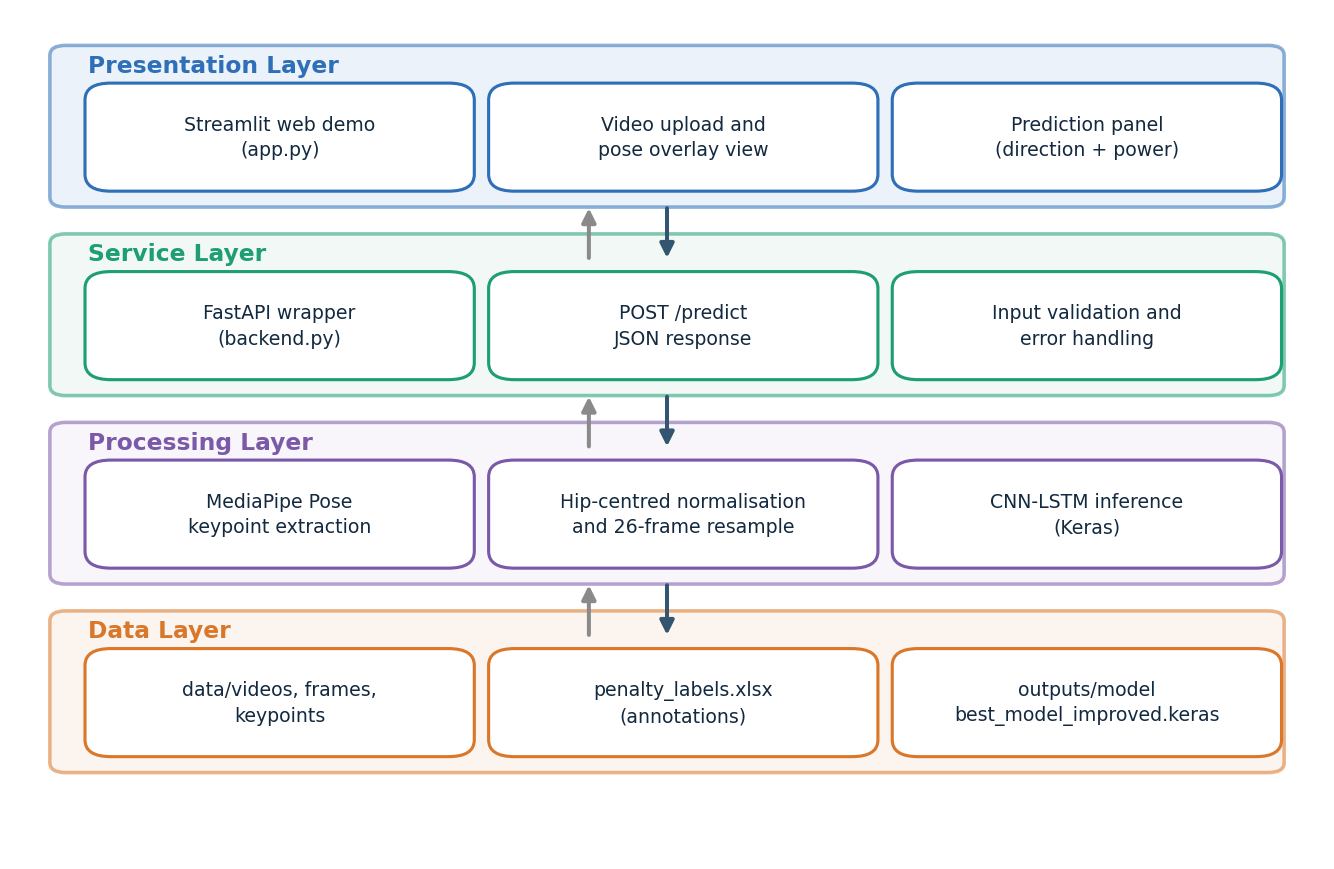
\includegraphics[width=0.99\textwidth]{fig04_system_architecture.png}
    \caption{Layered system architecture of KickSense}
    \label{fig:architecture}
\end{figure}

\noindent
\textbf{Description:} This diagram shows the four layers and the direction of their dependencies. Downward arrows indicate calls into the layer below and upward arrows indicate returned results. The presentation and service layers both route through the identical processing layer code path, which is the mechanism that prevents the preprocessing of an uploaded clip from drifting away from the preprocessing applied during training.

\section{Design Constraints}

\begin{itemize}
    \item \textbf{Hardware constraint:} the entire pipeline, including training, must run on a consumer laptop without a dedicated graphics processor. This single constraint rules out three dimensional convolution over pixel volumes and rules out the heavier pose estimators, and it is the reason the model is limited to roughly a quarter of a million parameters.
    \item \textbf{Input constraint:} the system must accept ordinary single camera video with no calibration, no known camera position and no depth sensor. Any representation that depends on knowing where the camera is cannot be used.
    \item \textbf{Data constraint:} no public dataset supervises this task, so the amount of labelled data is bounded by what could be manually annotated within the project timeline. Two hundred and twenty five usable sequences is the working figure, and every architectural decision was taken with that number in mind.
    \item \textbf{Software environment:} Python 3.12 inside a dedicated virtual environment named \texttt{kicksense\_env}, with TensorFlow and Keras for modelling, MediaPipe for pose estimation, OpenCV for video decoding, scikit-learn for splitting and metrics, pandas and openpyxl for the annotation file, and matplotlib for figure generation.
    \item \textbf{Reproducibility constraint:} all random seeds are fixed, the train, validation and test split is deterministic given a fixed random state, and all intermediate artefacts persist on disk, so that any reported number can be regenerated.
    \item \textbf{Honesty constraint:} the system must report its own failure rate rather than silently degrading. This is why the pose quality gate exists and why its rejection count is reported in Chapter 4 rather than omitted.
\end{itemize}

\section{Design Methodology}

The project follows an incremental, artefact driven methodology in which each stage is completed and persisted before the next begins. The reasoning is that the expensive and irreversible work in this project is data collection and annotation, not modelling, so the pipeline was deliberately built so that modelling experiments are cheap and repeatable while data work is done once.

\begin{itemize}
    \item \textbf{Partitioning:} the pipeline is decomposed into single responsibility scripts, namely frame extraction, pose estimation, preprocessing, training, and evaluation. Each is executable independently and each consumes only files written by an earlier stage.
    \item \textbf{Shared constants:} preprocessing constants such as the sequence length, the minimum detected frame count and the minimum detection ratio are declared once and imported wherever they are needed, which prevents the training and inference paths from diverging.
    \item \textbf{Deterministic splitting:} the train, validation and test partition is produced by a stratified split with a fixed random state, so the same clips land in the same partition on every run and results across experiments remain comparable.
    \item \textbf{Ablation by substitution:} because the architecture is constructed by a single builder function parameterised by variant, augmentation and regularisation flags, an ablation configuration differs from the full model by exactly one argument, which is what makes the attribution in Chapter 4 valid.
\end{itemize}

\section{High Level Design of the Pipeline}

\begin{figure}[H]
    \centering
    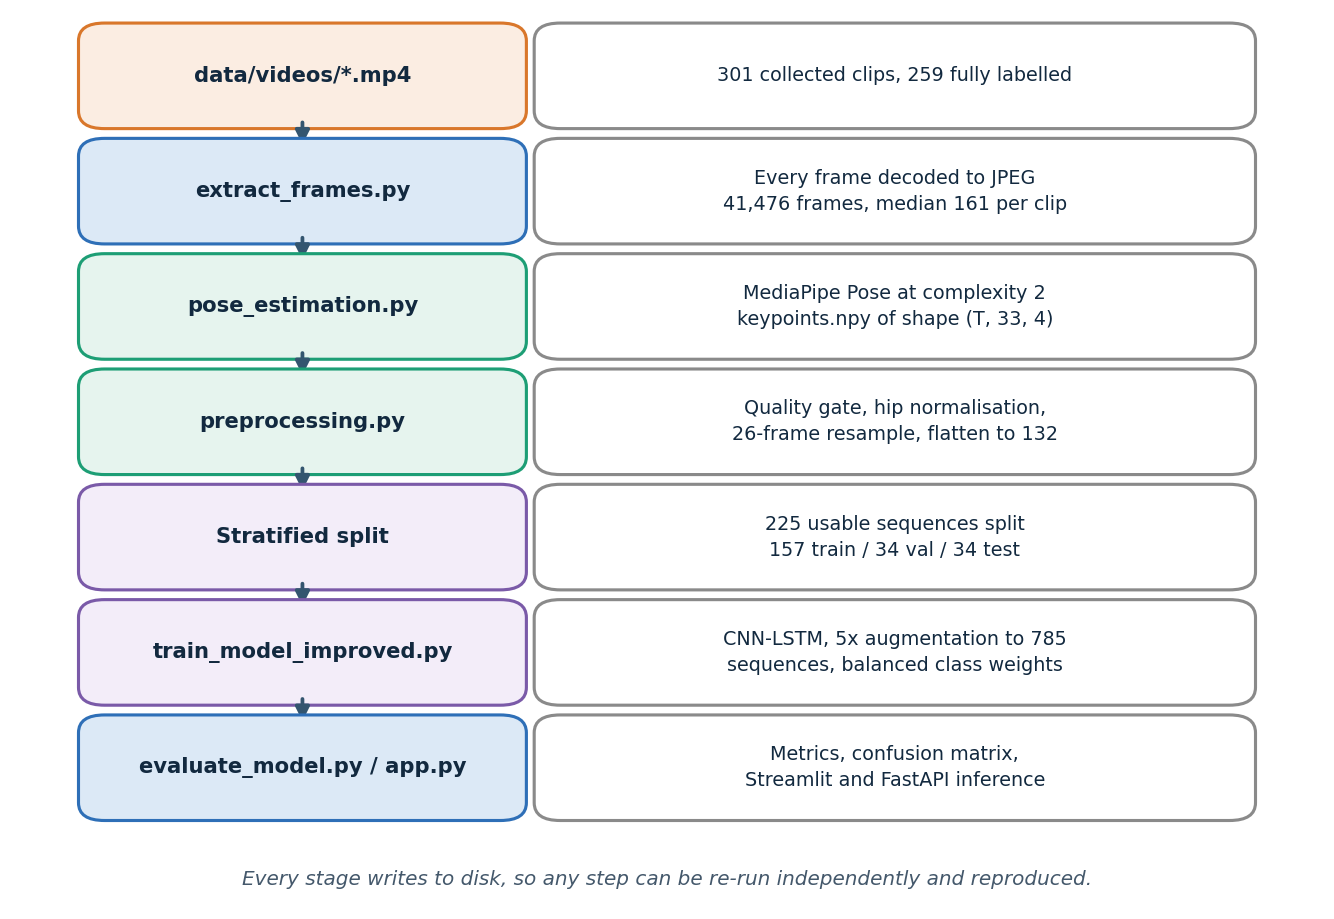
\includegraphics[width=0.92\textwidth]{fig05_pipeline_flow.png}
    \caption{End to end data pipeline from raw video to prediction}
    \label{fig:pipeline}
\end{figure}

\noindent
\textbf{Description:} This diagram traces the complete pipeline. The left column names the script or stage and the right column states what that stage produces, including the concrete quantities involved: three hundred and one collected clips reduced to two hundred and fifty nine annotated clips, variable length frame sequences reduced to a fixed twenty six step tensor, two hundred and twenty five usable sequences split into one hundred and fifty seven training, thirty four validation and thirty four test examples, and one hundred and fifty seven training sequences expanded to seven hundred and eighty five by fivefold augmentation.

\subsection{Stage One: Clip Preparation}

Source footage arrives in two forms. Broadcast material was obtained for penalties from a range of competitions and cut down so that each resulting file contains a single penalty, beginning shortly before the run up and ending shortly after contact. Locally recorded material was captured specifically for this project to increase the volume of the corpus and, more importantly, to add camera angles and framing that broadcast footage does not provide. The cutting was performed by a family of small scripts, each handling one source match, and the result is three hundred and one video files under \texttt{data/videos}.

\subsection{Stage Two: Frame Extraction}

Each video is decoded with OpenCV and every frame is written to disk as a JPEG image inside a per clip directory under \texttt{data/frames}. No subsampling is applied at this stage, deliberately, because discarding frames before pose estimation would discard information that the temporal resampling step is better placed to discard later, and because retaining all frames makes the detection ratio a meaningful diagnostic. Across the corpus this yields a mean of one hundred and sixty one frames per clip with a median of one hundred and sixty one, and the distribution together with the frame budget actually consumed is reported in Chapter 4.

\subsection{Stage Three: Pose Estimation}

Every extracted frame is passed through MediaPipe Pose. The configuration used is \texttt{static\_image\_mode=True}, \texttt{model\_complexity=2} and \texttt{min\_detection\_confidence=0.5}. The highest model complexity is chosen because accuracy of the landmark positions matters more than throughput in an offline batch stage. For each frame in which a pose is detected, the thirty three landmarks are recorded, each as four values, namely the horizontal coordinate normalised to the image width, the vertical coordinate normalised to the image height, a depth estimate relative to the hip midpoint, and a visibility confidence. Frames in which no pose is detected contribute nothing. The per clip result is an array of shape number of detected frames by thirty three by four, saved as \texttt{keypoints.npy} inside the clip directory under \texttt{data/keypoints}.

\begin{figure}[H]
    \centering
    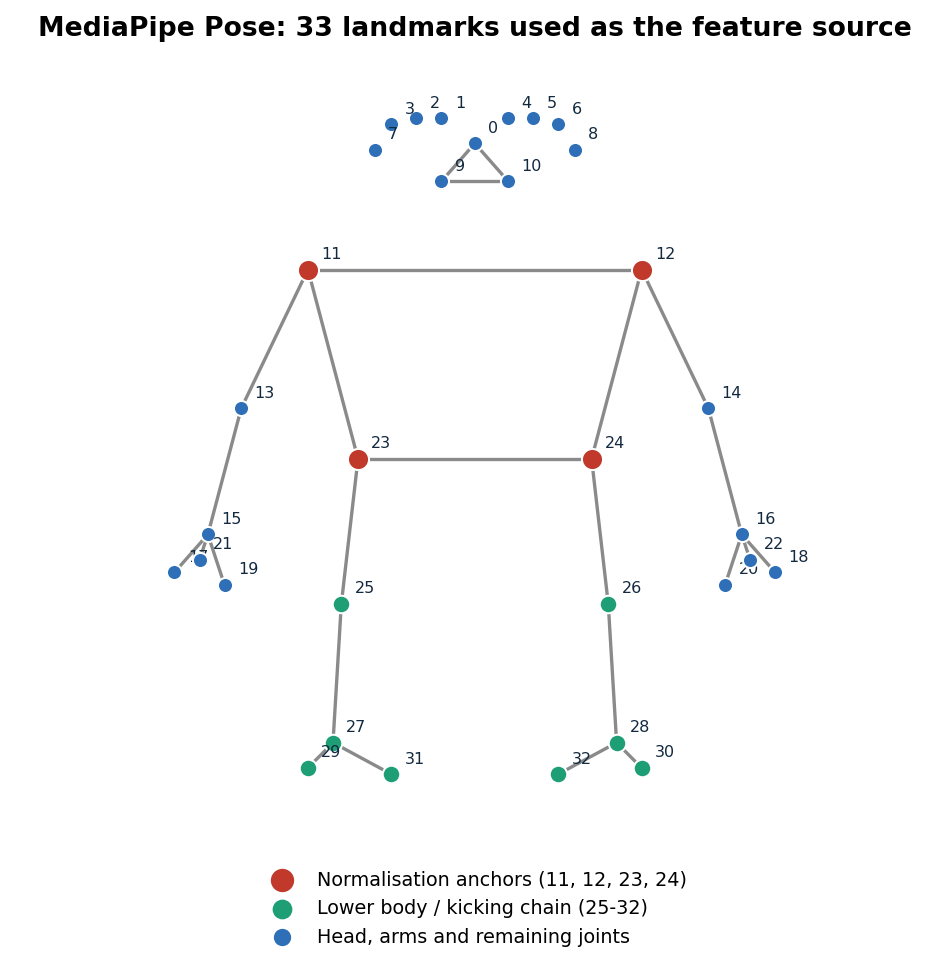
\includegraphics[width=0.72\textwidth]{fig07_mediapipe_landmarks.png}
    \caption{The 33 MediaPipe Pose landmarks and their role in KickSense}
    \label{fig:landmarks}
\end{figure}

\noindent
\textbf{Description:} This figure shows the landmark topology that defines the feature space. Landmarks eleven and twelve are the shoulders and landmarks twenty three and twenty four are the hips; these four are highlighted in red because they are used as the anchors for normalisation rather than merely as features. The lower body chain from landmark twenty five to landmark thirty two, highlighted in green, carries the kicking motion and is the region that both the perceptual literature and the base paper identify as most influential. The remaining landmarks are retained as features without playing a structural role.

\subsection{Stage Four: Preprocessing and Normalisation}

This stage converts variable length, camera dependent landmark streams into fixed size, camera independent tensors. It is the most consequential stage in the pipeline and proceeds in seven steps.

\begin{figure}[H]
    \centering
    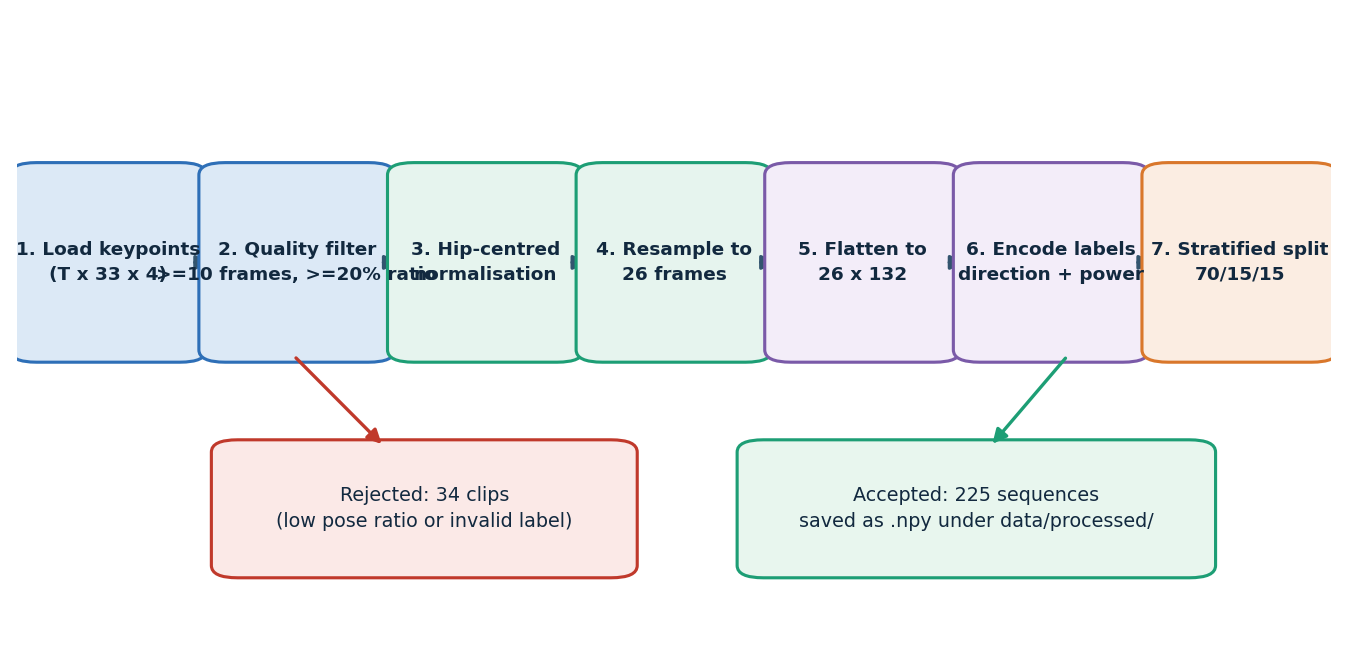
\includegraphics[width=0.99\textwidth]{fig08_preprocessing_flow.png}
    \caption{Preprocessing activity flow with the quality gate outcome}
    \label{fig:preprocessing}
\end{figure}

\noindent
\textbf{Description:} This activity diagram shows the seven preprocessing steps and, critically, the two possible outcomes of the quality gate. Clips that pass are written to \texttt{data/processed} as model ready sequences, and clips that fail are rejected and excluded from all subsequent stages, which is what converts a hidden pose estimation failure into a counted and reported quantity.

\begin{enumerate}[label=\arabic*.]
    \item \textbf{Load the landmark array.} The saved array of shape number of detected frames by thirty three by four is read from disk together with the total number of extracted frames for that clip, which is needed to compute the detection ratio.

    \item \textbf{Apply the quality gate.} A clip is rejected if it contains fewer than \texttt{MIN\_DETECTED\_FRAMES}, set to ten, or if the ratio of detected frames to extracted frames falls below \texttt{MIN\_POSE\_RATIO}, set to 0.20. The absolute threshold guards against clips too short to resample meaningfully, and the ratio threshold guards against clips in which MediaPipe succeeded only sporadically, since such clips produce a skeleton stream with large temporal gaps that resampling would paper over by interpolating across genuinely unobserved motion.

    \item \textbf{Normalise for camera position and player scale.} For each frame independently, the midpoint of the two hip landmarks, twenty three and twenty four, is computed and subtracted from every landmark, which places the origin at the player's pelvis and removes any dependence on where in the frame the player stands. A torso height is then computed as the vertical distance between the shoulder midpoint, from landmarks eleven and twelve, and the hip midpoint, and every coordinate is divided by that length, which removes the apparent size of the player and therefore the distance from the camera. What survives this operation is the shape of the body and how that shape changes over time, expressed in units of the player's own torso.

    \item \textbf{Resample to a fixed length.} Clips have different durations and different frame rates, so the detected frame sequence is resampled to exactly \texttt{SEQUENCE\_LENGTH}, set to twenty six, time steps by linear index interpolation. Sequences longer than twenty six frames are subsampled across their whole duration rather than truncated, so the run up, the plant and the strike are all represented; sequences shorter than twenty six frames are interpolated up. The value twenty six is a compromise between retaining enough temporal detail to distinguish the phases of the kick and keeping the input small enough that a quarter million parameter model is not immediately overparameterised.

    \item \textbf{Flatten to a feature vector.} The thirty three landmarks by four values per time step are flattened into a single vector of one hundred and thirty two features, producing a per clip tensor of shape twenty six by one hundred and thirty two. This is the exact input the model consumes.

    \item \textbf{Encode the labels.} The shot direction string is mapped to an integer, with left encoded as zero, centre as one and right as two, and is one hot encoded for the classification head. The shot power label is divided by ten so that it occupies the unit interval, which matches the sigmoid activation of the regression head, and predictions are multiplied by ten again at inference so that the reported value is on the original one to ten scale.

    \item \textbf{Split the dataset.} A stratified split with a fixed random state of forty two holds out fifteen percent as the test set, then splits the remainder with a proportion of 0.176 to produce the validation set, giving final sizes of one hundred and fifty seven training, thirty four validation and thirty four test sequences with the class proportions preserved in every partition.
\end{enumerate}

\subsection{Frames Extracted Against Frames Used}

The distinction between frames extracted and frames used matters and is easy to state precisely. Every frame of every clip is extracted and every extracted frame is submitted to MediaPipe, so pose estimation runs on the full corpus. The model, however, consumes exactly twenty six time steps per clip, so the temporal resampling step reduces a clip of one hundred and sixty one detected frames to twenty six representative steps. Averaged over the corpus this means roughly one sixth of the extracted frames contribute directly to a model input, with the remainder contributing indirectly by determining which frames the resampling selects and by establishing the detection ratio that the quality gate depends on. The exact totals across the whole corpus are reported in Chapter 4.

\begin{figure}[H]
    \centering
    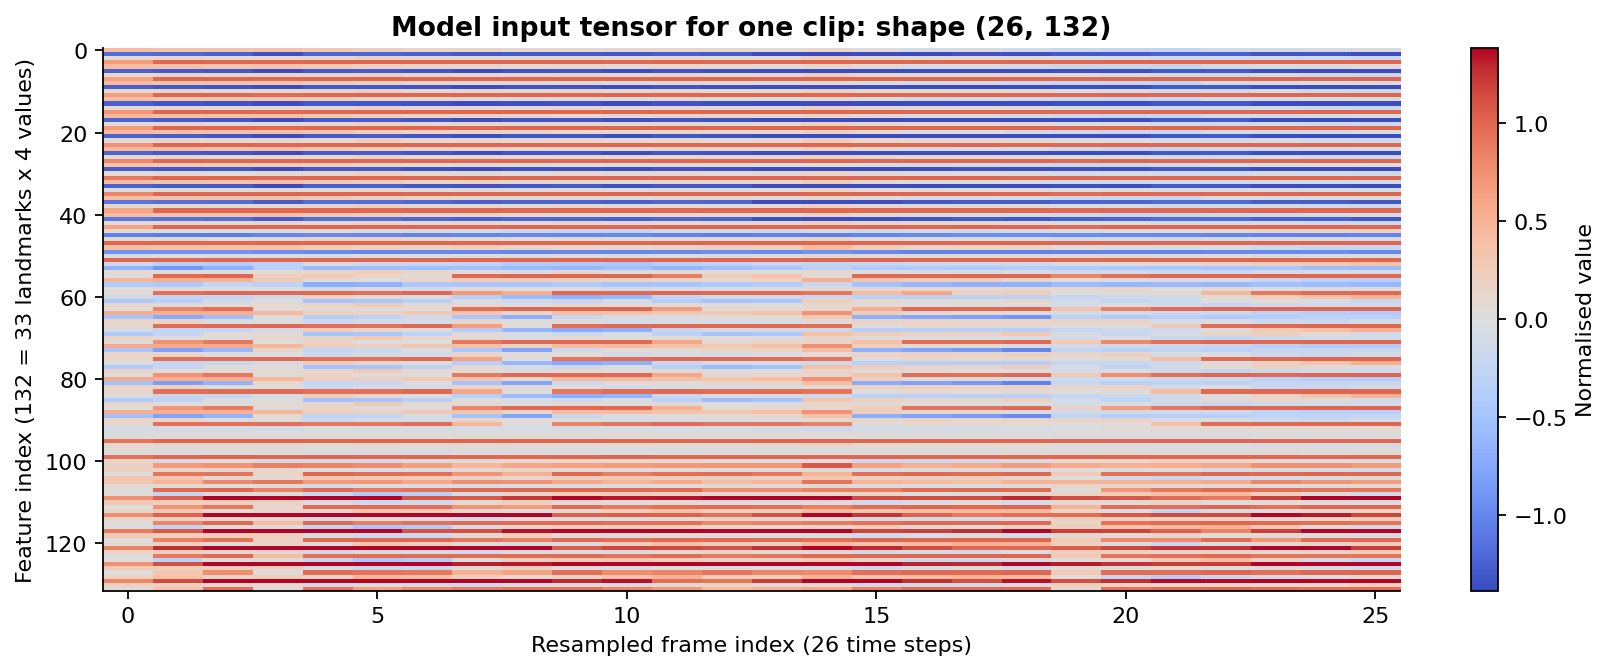
\includegraphics[width=0.99\textwidth]{fig27_feature_tensor.png}
    \caption{The model input tensor for a single clip, of shape 26 by 132}
    \label{fig:feature-tensor}
\end{figure}

\noindent
\textbf{Description:} This heatmap visualises one complete model input. The horizontal axis is the twenty six resampled time steps and the vertical axis is the one hundred and thirty two features, ordered as thirty three landmarks each contributing a horizontal coordinate, a vertical coordinate, a depth value and a visibility score. The horizontal banding shows that individual landmarks maintain a stable value across the sequence while specific rows, corresponding to the limbs involved in the kick, vary strongly over time. This variation is the signal the convolutional and recurrent layers are designed to detect.

\begin{figure}[H]
    \centering
    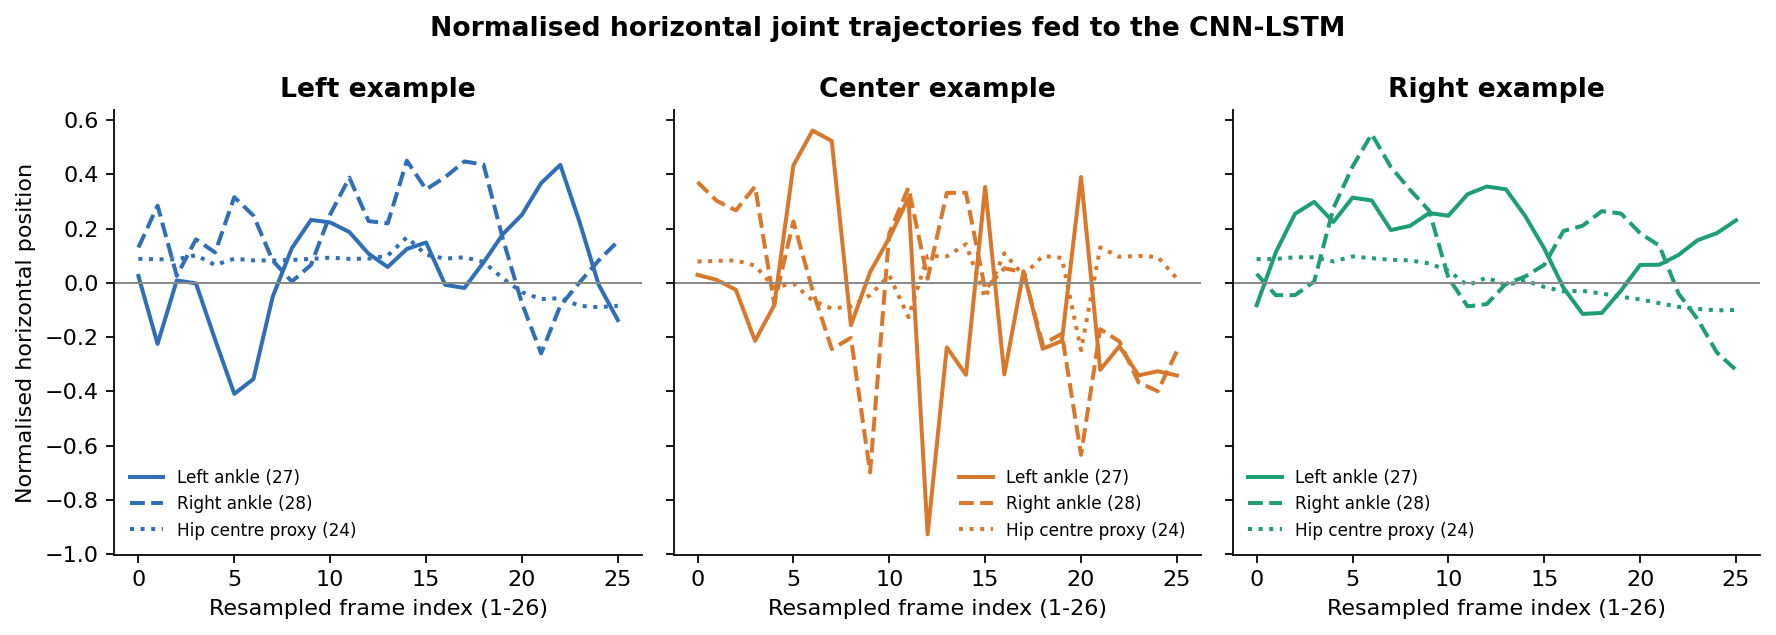
\includegraphics[width=0.99\textwidth]{fig26_pose_trajectories.png}
    \caption{Normalised horizontal joint trajectories for one example from each direction class}
    \label{fig:trajectories}
\end{figure}

\noindent
\textbf{Description:} This figure plots the normalised horizontal position of the two ankle landmarks and one hip landmark across the twenty six time steps, for one training example from each of the three direction classes. It demonstrates two things. First, the normalisation is working, because the trajectories are centred near zero and expressed on a comparable scale despite the source clips being filmed differently. Second, the classes are not trivially separable, since the trajectories overlap substantially, which is consistent with the moderate accuracy reported in Chapter 4 and explains why a temporal model rather than a simple threshold on a single landmark is required.

\section{Low Level Design of the Model}

\subsection{Architecture}

The model is a multi task network with a shared encoder and two task specific heads. The encoder combines one dimensional convolution with stacked recurrence, which reflects a specific hypothesis about the data. The convolutional front end operates across the time axis with a kernel of width three, so each filter observes three consecutive time steps and learns short range local motion primitives such as the acceleration of a limb or a change in the direction of a joint's travel. The recurrent back end then integrates these primitives over the full sequence, which is what allows the model to represent the ordering of the phases of the kick rather than merely their presence.

\begin{figure}[H]
    \centering
    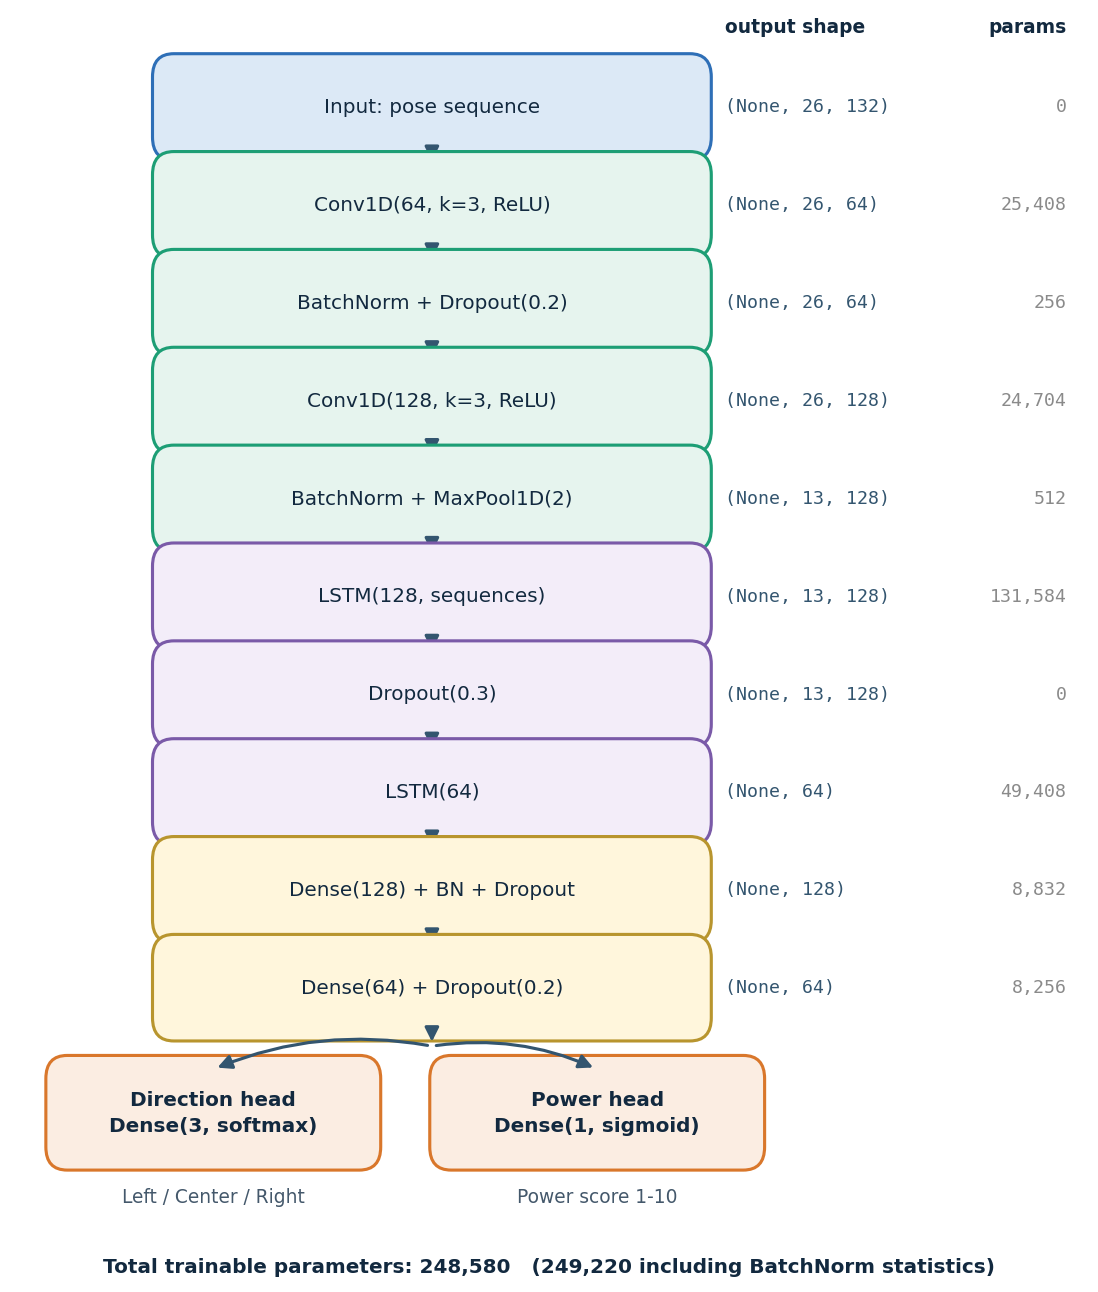
\includegraphics[width=0.80\textwidth]{fig06_model_architecture.png}
    \caption{Layer by layer architecture of the multi-task CNN-LSTM with tensor shapes and parameter counts}
    \label{fig:model}
\end{figure}

\noindent
\textbf{Description:} This diagram gives the complete architecture with the output shape and parameter count of every layer. The input of twenty six by one hundred and thirty two passes through two convolutional blocks that expand the channel dimension from one hundred and thirty two to sixty four and then to one hundred and twenty eight while max pooling halves the temporal dimension from twenty six to thirteen. Two stacked recurrent layers reduce the sequence to a single sixty four dimensional vector, two dense layers refine it, and the representation then branches into a three way softmax head for direction and a single unit sigmoid head for power. The total is 249,220 parameters of which 248,580 are trainable, the remaining 640 being the non trainable running statistics of the batch normalisation layers.

The two heads share the entire encoder, which is the central design decision of the model. The reasoning is sample efficiency. The body motion that determines where the ball is going is the same motion that determines how hard it will be struck, so training two separate networks on two hundred and twenty five sequences would learn the same representation twice from half as much effective supervision. Sharing the encoder means the direction labels also contribute gradient signal to the features the power head uses, and vice versa.

\subsection{Loss Function}

Training minimises a weighted sum of two losses computed on the two heads:
\[
\mathcal{L} = \lambda_{d}\,\mathcal{L}_{\text{CE}}(y_{d}, \hat{y}_{d}) \;+\; \lambda_{p}\,\mathcal{L}_{\text{MSE}}(y_{p}, \hat{y}_{p})
\]
where the direction term is the categorical cross entropy over the three classes,
\[
\mathcal{L}_{\text{CE}}(y_{d}, \hat{y}_{d}) = -\sum_{c=1}^{3} y_{d,c}\log \hat{y}_{d,c}
\]
and the power term is the mean squared error on the unit interval,
\[
\mathcal{L}_{\text{MSE}}(y_{p}, \hat{y}_{p}) = \frac{1}{N}\sum_{i=1}^{N}\left(\frac{p_{i}}{10} - \hat{p}_{i}\right)^{2}.
\]
The weights are set to $\lambda_{d} = 1.0$ and $\lambda_{p} = 0.3$. The asymmetry is deliberate and follows directly from the data. Direction is objectively verifiable from the footage and is the primary deliverable, whereas the power label is a subjective human judgement on a coarse ordinal scale and therefore carries substantial noise. Weighting the power term at three tenths allows it to shape the shared representation without allowing a noisy target to dominate the gradient and degrade the classification the system is primarily judged on.

\subsection{Class Weighting}

Balanced class weights are computed from the augmented training labels using the standard inverse frequency formulation, in which the weight of class $c$ is
\[
w_{c} = \frac{N}{K \cdot n_{c}}
\]
with $N$ the total number of training samples, $K$ the number of classes and $n_{c}$ the count of class $c$. One implementation detail is worth recording because it materially affects the interpretation of results. Keras does not accept a \texttt{class\_weight} argument for a model with more than one output, so the production training script computes these weights but does not in fact apply them during fitting. For the controlled experiments reported in Chapter 4 the weights are instead applied as per sample weights attached to the direction head, which is the functionally equivalent mechanism that Keras does support for multi output models. This is why the ablation table contains an explicit row with and without class weighting, and why the configuration matching the production script is the one labelled as omitting them.

\subsection{Data Augmentation}

The one hundred and fifty seven training sequences are expanded fivefold to seven hundred and eighty five by generating four additional variants of every sequence. Augmentation is applied to the training partition only; the validation and test partitions remain untouched.

\begin{itemize}
    \item \textbf{Gaussian noise.} Zero mean noise with a standard deviation of 0.01 is added to every coordinate, which models the jitter that a pose estimator produces on real footage and discourages the model from depending on landmark positions to a precision the estimator does not deliver.
    \item \textbf{Uniform scaling.} The whole sequence is multiplied by a factor drawn uniformly from 0.95 to 1.05, providing residual invariance to player build beyond what torso normalisation already removes.
    \item \textbf{Horizontal mirroring with label inversion.} The horizontal coordinate of every landmark is negated and the sixteen anatomically left and right paired landmarks are swapped, producing a valid pose of a mirrored player. The direction label is inverted accordingly, so a left shot becomes a right shot and a right shot becomes a left shot, while a centre shot remains centre. This is the most valuable of the four transformations because it is the only one that is label changing rather than label preserving, so it generates genuinely new class examples rather than perturbed copies, and it directly counteracts any left or right asymmetry in the corpus.
    \item \textbf{Temporal shift.} The sequence is circularly shifted by one or two time steps, which removes the assumption that the phases of the kick are aligned to the same absolute frame indices in every clip.
\end{itemize}

\subsection{Regularisation}

Because a quarter million parameter model trained on a few hundred sequences will overfit by default, several regularisation mechanisms operate together. Batch normalisation is applied after each convolutional block and after the first dense layer, which stabilises the scale of activations and permits a usable learning rate. Dropout is applied at rates of 0.2 after the convolutional blocks, 0.3 after each recurrent layer and after the first dense layer, and 0.2 after the second dense layer. Max pooling halves the temporal dimension after the second convolutional block, which reduces the parameter count of the subsequent recurrent layer. Early stopping monitors validation direction accuracy with a patience of twenty epochs and restores the weights from the best epoch, so the reported model is never the final epoch's model but the best generalising one observed. A learning rate reduction on plateau halves the learning rate after eight epochs without improvement in validation direction loss, down to a floor of one times ten to the power of minus five.

\section{Tools and Technologies}

\renewcommand{\arraystretch}{1.25}
\small
\begin{longtable}{|>{\bfseries}p{3.4cm}|p{4.0cm}|p{5.6cm}|}
\hline
\textbf{Component} & \textbf{Technology} & \textbf{Role in KickSense} \\ \hline
\endfirsthead
\hline
\textbf{Component} & \textbf{Technology} & \textbf{Role in KickSense} \\ \hline
\endhead
\hline
\multicolumn{3}{r}{\textit{Continued on next page}} \\
\hline
\endfoot
\hline
\endlastfoot
Language & Python 3.12 & All pipeline stages, training and interfaces \\ \hline
Environment & \texttt{kicksense\_env} virtual environment & Isolates dependencies and pins versions \\ \hline
Pose estimation & MediaPipe Pose (BlazePose) & Extracts 33 landmarks per frame at model complexity two \\ \hline
Video decoding & OpenCV & Frame extraction and metadata such as resolution and frame rate \\ \hline
Deep learning & TensorFlow with Keras & Model construction, training, checkpointing and inference \\ \hline
Numerical computing & NumPy & Landmark arrays, normalisation, resampling and augmentation \\ \hline
Data handling & pandas with openpyxl & Reading and writing the annotation spreadsheet \\ \hline
Machine learning utilities & scikit-learn & Stratified splitting, balanced class weights, all reported metrics \\ \hline
Visualisation & matplotlib & Every figure in this report, generated from project artefacts \\ \hline
Demonstration interface & Streamlit & Clip upload, pose overlay rendering and prediction display \\ \hline
Service interface & FastAPI & HTTP inference endpoint for the planned mobile client \\ \hline
Planned client & Flutter for web and Android & Designed but not implemented; listed in future work \\ \hline
Version control & Git & Full history of code, annotations and outputs \\ \hline
Editor & VS Code & Development environment \\ \hline
\caption{Tools and technologies used in the project and their specific role}
\label{tab:tools}
\end{longtable}
\normalsize

\noindent
\textbf{Description:} This table lists every technology in the stack together with the precise function it performs, so that no component appears without a stated purpose. The final two rows are included for completeness and are explicitly marked as designed rather than delivered.

\section{Where Each Model and Technique Is Applied}

\renewcommand{\arraystretch}{1.25}
\small
\begin{longtable}{|>{\bfseries}p{3.6cm}|p{3.4cm}|p{6.0cm}|}
\hline
\textbf{Technique} & \textbf{Applied at stage} & \textbf{Reason it is applied there} \\ \hline
\endfirsthead
\hline
\textbf{Technique} & \textbf{Applied at stage} & \textbf{Reason it is applied there} \\ \hline
\endhead
\hline
\multicolumn{3}{r}{\textit{Continued on next page}} \\
\hline
\endfoot
\hline
\endlastfoot
MediaPipe Pose & Stage 3, pose estimation & Reduces each frame from pixels to 132 numbers, removing all appearance variation \\ \hline
Quality gate & Stage 4, step 2 & Rejects clips whose pose stream is too sparse to resample honestly \\ \hline
Hip-centred translation & Stage 4, step 3 & Removes the player's position in frame, which carries no directional information \\ \hline
Torso-height scaling & Stage 4, step 3 & Removes apparent player size, which encodes camera distance rather than technique \\ \hline
Linear resampling & Stage 4, step 4 & Removes dependence on clip duration and frame rate \\ \hline
Conv1D layers & Model encoder, front end & Learn short-range local motion primitives over three consecutive time steps \\ \hline
Max pooling & Model encoder, after block two & Halves the temporal dimension and shrinks the following recurrent layer \\ \hline
LSTM layers & Model encoder, back end & Integrate local primitives into an ordered representation of the whole kick \\ \hline
Batch normalisation & After conv blocks and dense one & Stabilises activation scale and permits a usable learning rate \\ \hline
Dropout & After every major block & Suppresses overfitting on a small dataset \\ \hline
Softmax head & Model output, direction & Produces a normalised distribution over Left, Center and Right \\ \hline
Sigmoid head & Model output, power & Constrains the regression to the unit interval matching the scaled label \\ \hline
Weighted multi-task loss & Training objective & Lets the noisy power target inform the encoder without dominating it \\ \hline
Balanced class weights & Training, direction head & Compensates for the 107 / 58 / 94 class imbalance \\ \hline
Mirror augmentation & Training data only & Generates genuinely new class examples and removes left-right asymmetry \\ \hline
Early stopping & Training control & Selects the best generalising epoch rather than the last one \\ \hline
Stratified split & Stage 4, step 7 & Guarantees every class is represented in every partition \\ \hline
\caption{Mapping of every technique to the pipeline stage where it is applied and the reason for it}
\label{tab:where-used}
\end{longtable}
\normalsize

\noindent
\textbf{Description:} This table exists to answer the question of where each technique actually operates, since several of them could in principle be placed at more than one stage. Reading the middle column top to bottom traces the pipeline in execution order, and the right column states the specific problem each technique is present to solve.

\section{Training Configuration}

\renewcommand{\arraystretch}{1.25}
\small
\begin{longtable}{|>{\bfseries}p{5.2cm}|p{4.0cm}|p{4.0cm}|}
\hline
\textbf{Hyperparameter} & \textbf{Value} & \textbf{Note} \\ \hline
\endfirsthead
\hline
\textbf{Hyperparameter} & \textbf{Value} & \textbf{Note} \\ \hline
\endhead
\hline
\multicolumn{3}{r}{\textit{Continued on next page}} \\
\hline
\endfoot
\hline
\endlastfoot
Input shape & (26, 132) & 26 time steps, 132 features \\ \hline
Optimiser & Adam & \\ \hline
Initial learning rate & 0.0005 & Halved on plateau \\ \hline
Batch size & 16 & Small, to suit 785 samples \\ \hline
Maximum epochs & 150 & Rarely reached \\ \hline
Direction loss & Categorical cross entropy & Weight 1.0 \\ \hline
Power loss & Mean squared error & Weight 0.3 \\ \hline
Early stopping monitor & Validation direction accuracy & Patience 20, best weights restored \\ \hline
Learning rate schedule & Reduce on plateau, factor 0.5 & Patience 8, minimum 1e-5 \\ \hline
Dropout rates & 0.2 / 0.3 / 0.3 / 0.2 & Conv, LSTM, dense one, dense two \\ \hline
Augmentation factor & 5 times & 157 sequences become 785 \\ \hline
Class weighting & Balanced, inverse frequency & Applied as sample weights \\ \hline
Random seed & 42 & Python, NumPy and TensorFlow \\ \hline
Total parameters & 249,220 & 248,580 trainable \\ \hline
\caption{Training hyperparameters used for every experiment reported in Chapter 4}
\label{tab:hyperparams}
\end{longtable}
\normalsize

\noindent
\textbf{Description:} These are the settings held constant across every experiment in the following chapter, so that any difference in a reported result is attributable to the single factor being varied rather than to an incidental change of configuration. Systematic tuning of these values has deliberately not been attempted yet and is listed as future work in Chapter 5.

\section{Inference Path}

\begin{figure}[H]
    \centering
    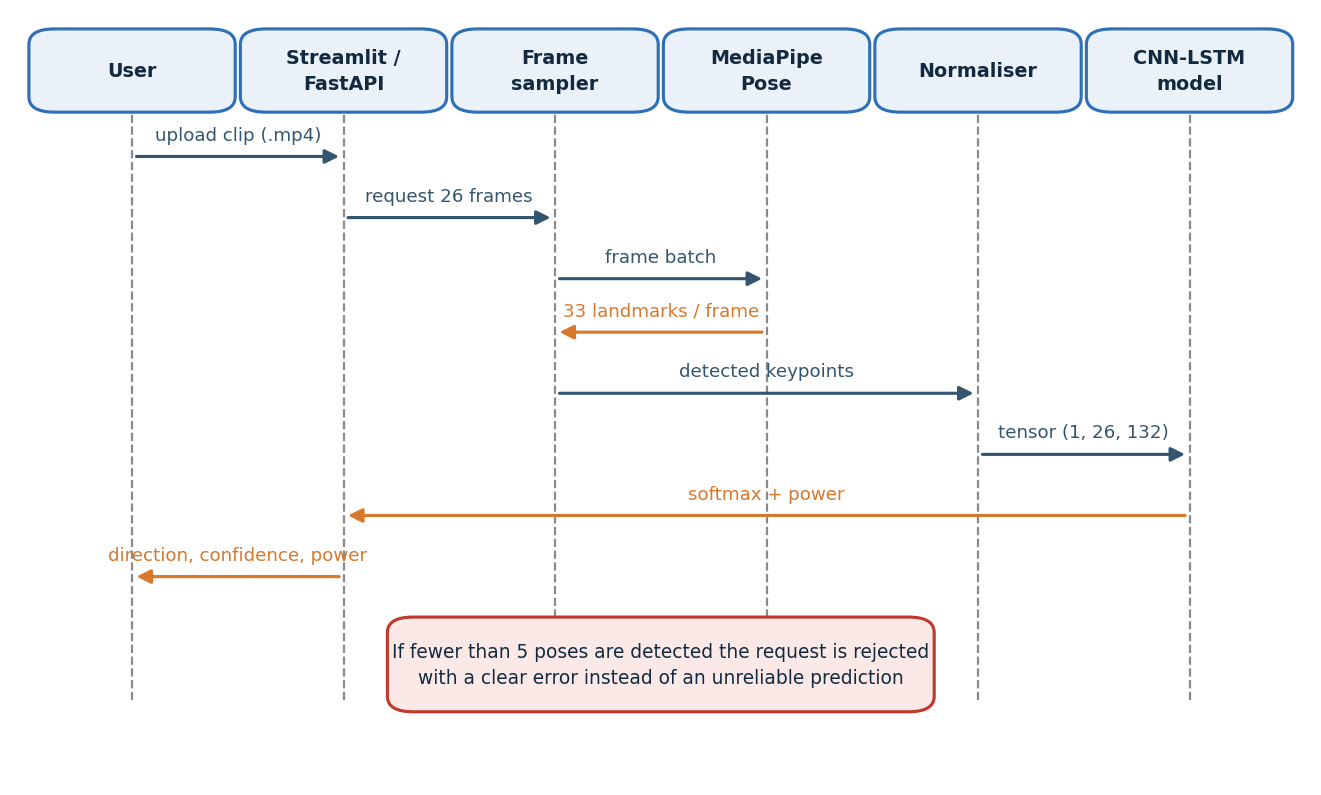
\includegraphics[width=0.99\textwidth]{fig09_inference_sequence.png}
    \caption{Sequence diagram of the inference path for an uploaded clip}
    \label{fig:inference}
\end{figure}

\noindent
\textbf{Description:} This sequence diagram traces a single prediction request. The user uploads a clip, the interface requests a frame sample, MediaPipe returns landmarks for each frame, the normaliser produces a tensor of shape one by twenty six by one hundred and thirty two, and the model returns a softmax distribution together with a power value. The guard shown at the bottom is important: if too few poses are detected the request is refused with an explicit error rather than answered with a prediction derived from an unusable skeleton stream, which mirrors at inference time the quality gate applied during training.

\section{Experiments Conducted}

Two distinct families of experiment are reported in Chapter 4, and it is worth separating them clearly because they answer different questions.

The first family is the development history, comprising five complete training runs whose logs are preserved in \texttt{outputs/model}. These runs differ from one another in the state of the annotation file and in the correctness of the pipeline at the time they were executed, since the corpus grew as locally recorded footage was added, a defect in the mirror augmentation was identified and corrected, and a portion of the direction labels was re-verified against the footage. These runs therefore document how the result improved as the data and the code improved, and the highest validation direction accuracy observed anywhere in the project, 55.9 percent at epoch twenty nine, comes from this family.

The second family is the controlled ablation study, comprising six configurations trained under identical conditions with a fixed seed on the current data, differing from the full model by exactly one factor each. These runs answer the question of which design decisions actually contribute, and because they share a seed and a split they support attribution in a way the development history cannot. The reference model used for every test set number and every evaluation figure in Chapter 4 is the full configuration from this second family, so that the confusion matrix, the per class metrics and the power regression plots all describe one single reproducible checkpoint rather than a mixture of runs.

\clearpage


\chapter{Dataset and Experimental Evaluation}
This chapter describes the dataset that KickSense was built on and reports the results obtained from it. It opens with the composition and characteristics of the corpus, including the properties that make it difficult, then presents the qualitative evaluation, which examines whether the pose extraction is visually faithful and where it fails, and then the quantitative evaluation, which reports the metrics obtained on a held out test split that was never used for model selection. The chapter closes with the ablation study, the development history across all recorded runs, and a comparison of the evaluation protocol against that of the base paper. Every number quoted here is computed by the scripts in \texttt{report\_assets} from the artefacts in the repository, and every figure was generated by the same run that produced the numbers.

\section{Which Dataset Is Used}

No public dataset annotates the direction of a football penalty kick, as established in Chapter 2, so the corpus used here was collected and annotated specifically for this project. It has two distinct components, and the difference between them turns out to be one of the most informative findings in the whole evaluation.

The first component is broadcast footage. Penalties were sourced from recorded matches across seventeen competitions, including the men's World Cup 2022, the Women's World Cup 2023, AFCON 2025, the Leagues Cup 2023, the Champions League 2008, Euro 2020, Euro 2024 and the FA Cup 2022, and each source match was cut into individual single penalty clips. This component provides breadth of players, stadiums and techniques, and it is the only realistic way to obtain elite level penalties at volume.

The second component is footage recorded specifically for this project. Sixty one clips were captured during dedicated local sessions, framed so that the kicker occupies a substantial part of the image and is not occluded. This component was added to increase the size of the corpus, but its more important contribution is that it provides the camera framing that broadcast footage does not, which as Section 4.5 shows is the single largest determinant of whether pose estimation succeeds at all.

\section{Dataset Insights}

\subsection{Media Type, Volume and Acquisition Properties}

The dataset is video rather than still imagery, which is essential rather than incidental. A single frame of a penalty run up cannot distinguish a player who is about to open the hips from a player who is about to close them, because the discriminative information is in how the body configuration changes over time rather than in any one configuration. Every clip must therefore be treated as a temporal sequence, and the modelling problem is sequence classification rather than image classification.

\renewcommand{\arraystretch}{1.25}
\small
\begin{longtable}{|>{\bfseries}p{6.4cm}|p{7.4cm}|}
\hline
\textbf{Property} & \textbf{Value} \\ \hline
\endfirsthead
\hline
\textbf{Property} & \textbf{Value} \\ \hline
\endhead
\hline
\multicolumn{2}{r}{\textit{Continued on next page}} \\
\hline
\endfoot
\hline
\endlastfoot
Media type & Video, single camera, no depth channel \\ \hline
Video files collected & 301 \\ \hline
Clips with complete annotation & 259 \\ \hline
Clips with a saved keypoint array & 257 \\ \hline
Sequences usable after the quality gate & 225 \\ \hline
Resolutions present & 1280 by 720 (164 files), 640 by 360 (137 files) \\ \hline
Frame rates present & 25 fps (184 files), 30 fps (109 files), 50 fps (8 files) \\ \hline
Colour format & 3 channel RGB, no depth or infrared \\ \hline
Extracted frames per clip, mean & 161 \\ \hline
Extracted frames per clip, median & 161 \\ \hline
Extracted frames per clip, range & 1 to 2,495 \\ \hline
Total frames extracted across the corpus & 41,476 \\ \hline
Total frames in which a pose was detected & 25,167 \\ \hline
Total frames actually consumed by the model & 6,526 (15.7 percent of extracted) \\ \hline
Sequence length after resampling & 26 time steps \\ \hline
Features per time step & 132 (33 landmarks by 4 values) \\ \hline
Model input tensor shape & (26, 132) \\ \hline
Direction label counts & Left 107, Right 94, Center 58 \\ \hline
Outcome label counts & Goal 225, Saved 21, Missed 13 \\ \hline
Ball placement label counts & Top left 104, Center 85, Top right 60, Bottom right 6, Bottom left 3 \\ \hline
Dominant foot label counts & Right 253, Left 6 \\ \hline
Shot power scale & Integer 1 to 10, manually annotated \\ \hline
Distinct source competitions & 17 \\ \hline
Distinct players & 138 \\ \hline
Train / validation / test split & 157 / 34 / 34 sequences \\ \hline
\caption{Summary of the KickSense dataset and its acquisition properties}
\label{tab:dataset-summary}
\end{longtable}
\normalsize

\noindent
\textbf{Description:} This table gives the complete numerical description of the corpus in one place. Three rows deserve particular attention. The gap between 259 annotated clips and 225 usable sequences is the cost of the pose quality gate and is quantified in Section 4.5. The gap between 41,476 extracted frames and 6,526 consumed frames is the effect of temporal resampling, and it shows that only 15.7 percent of extracted frames reach the model directly, the remainder serving to determine which frames the resampling selects and to establish the detection ratio the quality gate depends on. The dominant foot distribution, at 253 right footed against 6 left footed, is so skewed that the model cannot learn anything foot specific, which is exactly why the mirror augmentation described in Chapter 3 is valuable.

\begin{figure}[H]
    \centering
    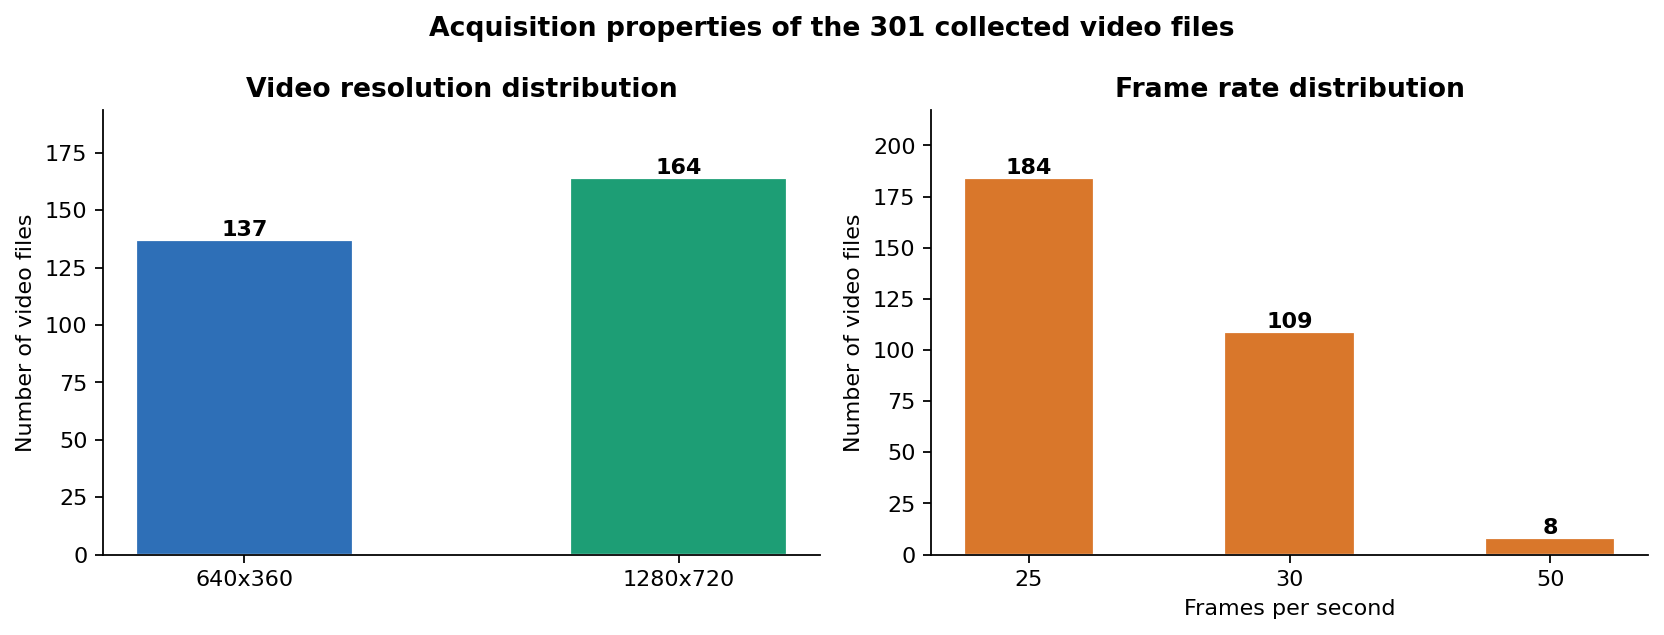
\includegraphics[width=0.99\textwidth]{fig12_resolution_framerate.png}
    \caption{Resolution and frame rate distribution across the 301 collected video files}
    \label{fig:resolution}
\end{figure}

\noindent
\textbf{Description:} The corpus is split between two resolutions and three frame rates, with no single setting dominating. This heterogeneity is the reason the preprocessing stage must normalise coordinates and resample time rather than assuming a fixed acquisition format. Because MediaPipe returns coordinates normalised to the image dimensions, resolution differences are absorbed automatically; frame rate differences are absorbed by the fixed length temporal resampling.

\subsection{Label Distribution}

\begin{figure}[H]
    \centering
    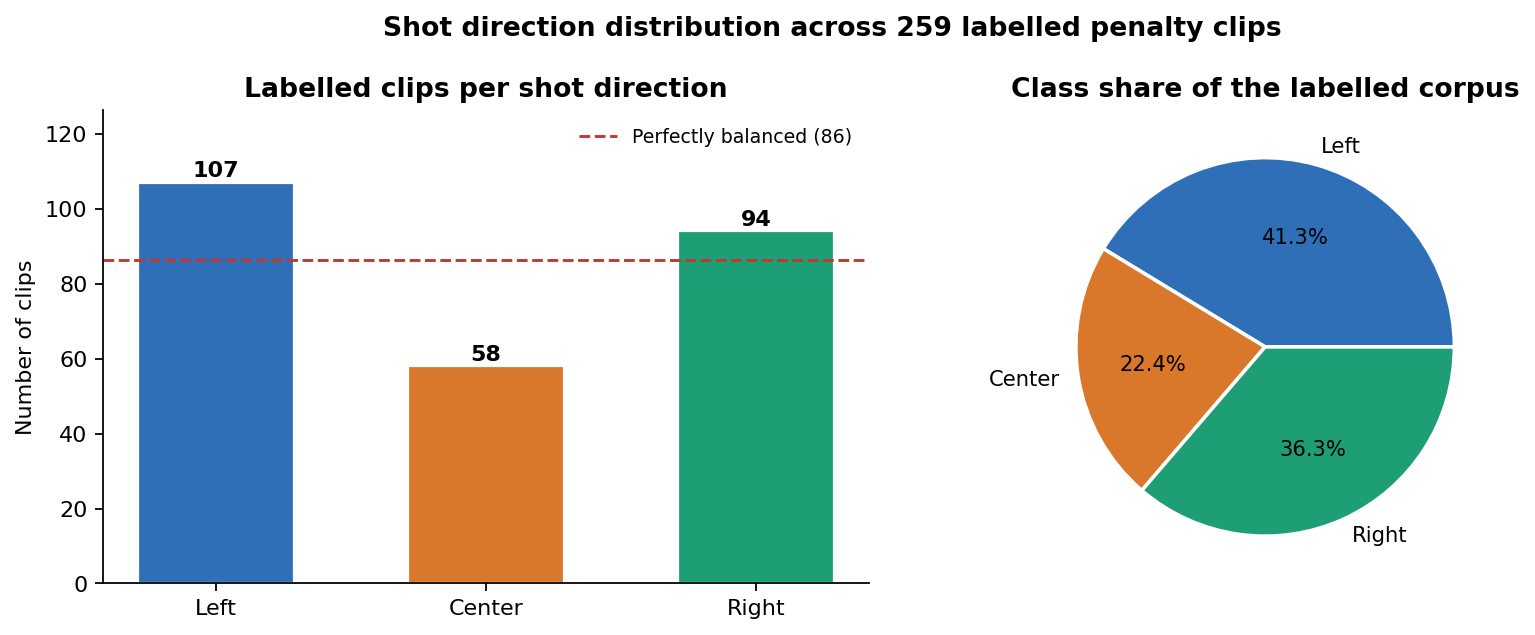
\includegraphics[width=0.99\textwidth]{fig10_class_distribution.png}
    \caption{Shot direction distribution across the 259 labelled penalty clips}
    \label{fig:class-dist}
\end{figure}

\noindent
\textbf{Description:} The three direction classes are unbalanced, with 107 left, 94 right and 58 centre examples against 86 that a perfectly balanced corpus would contain in each class. The imbalance is not an artefact of collection but a property of the sport, because penalty takers aim for the corners far more often than down the middle. The consequence is that the centre class has roughly half the support of the other two, and the per class metrics in Section 4.6 show precisely this effect.

\begin{figure}[H]
    \centering
    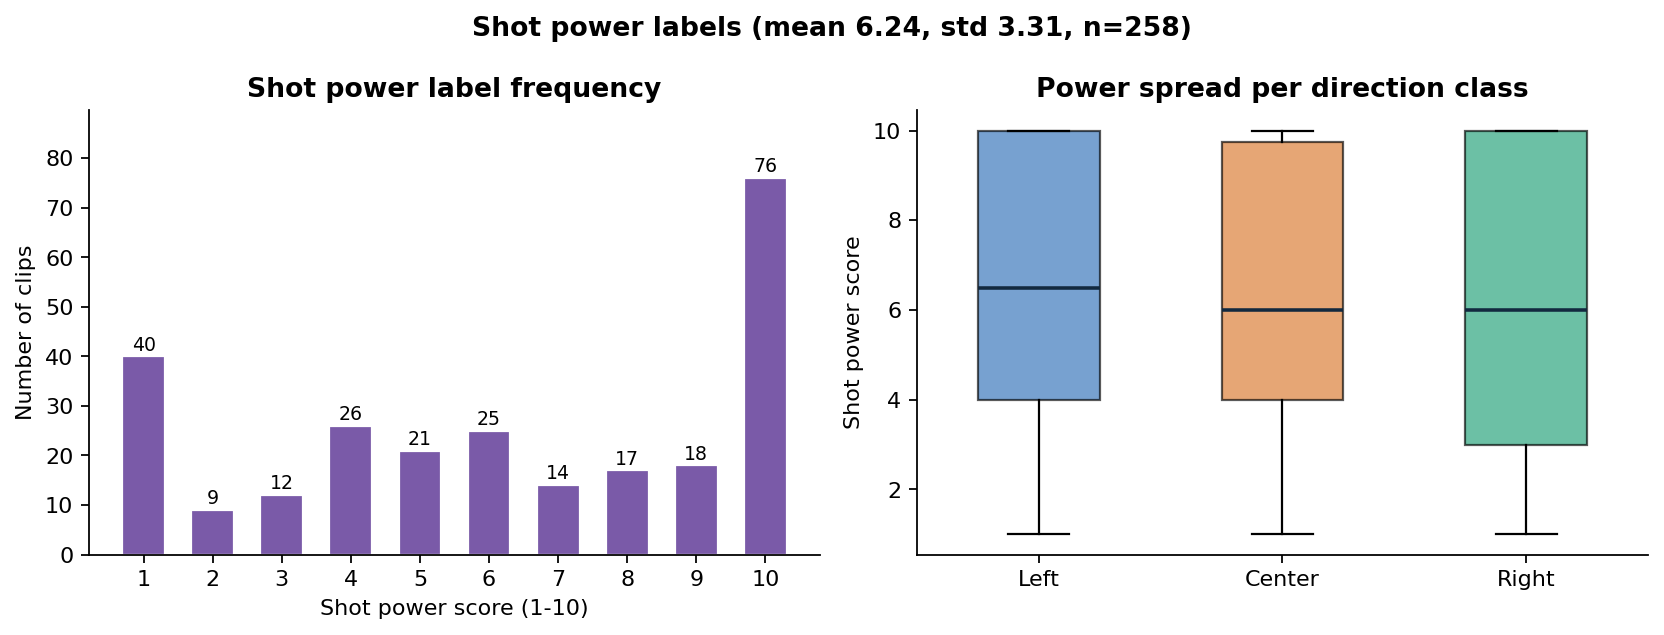
\includegraphics[width=0.99\textwidth]{fig11_power_distribution.png}
    \caption{Shot power label frequency and its spread within each direction class}
    \label{fig:power-dist}
\end{figure}

\noindent
\textbf{Description:} The left panel exposes a genuine weakness in the annotation. The power scale is nominally continuous from one to ten, but the observed distribution is strongly bimodal, with 76 clips at the maximum value of ten and 40 at the minimum value of one, which indicates that the annotator was in practice making a coarse categorical judgement rather than a graded one. The right panel shows that power is distributed almost identically across the three direction classes, with means of 6.48 for left, 6.17 for centre and 6.00 for right against standard deviations above 3.2 in every class. This is informative in two ways: it confirms that the direction label and the power label are close to statistically independent, so the multi task setup is not merely predicting the same quantity twice, and it means the power head has to work from motion characteristics alone with no help from the direction signal.

\begin{figure}[H]
    \centering
    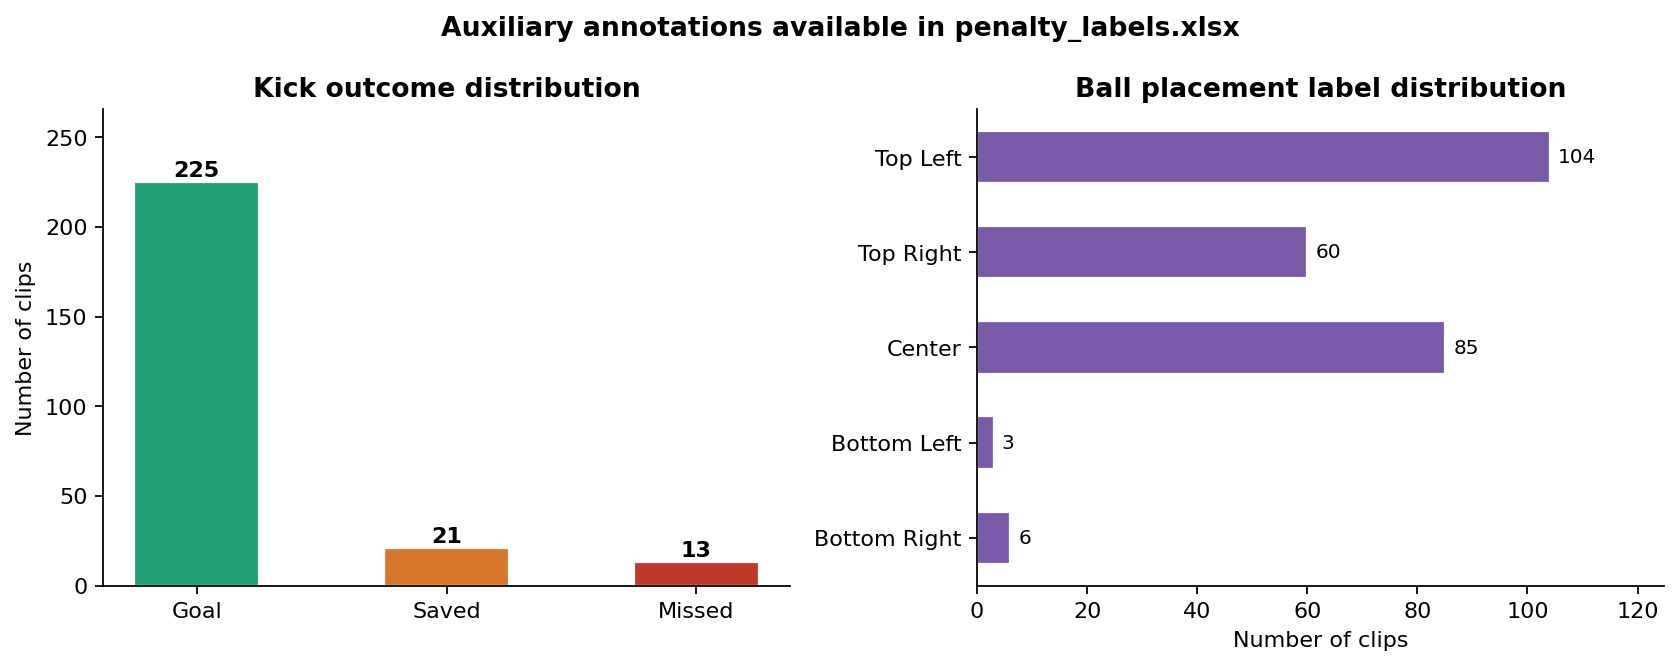
\includegraphics[width=0.99\textwidth]{fig16_outcome_placement.png}
    \caption{Kick outcome and ball placement annotations available in the label file}
    \label{fig:outcome}
\end{figure}

\noindent
\textbf{Description:} These two auxiliary annotations are present in the label file but are not currently consumed by the model. The outcome distribution is extremely skewed, with 225 goals against 21 saves and 13 misses, which reflects the fact that most penalties at elite level are scored and which makes outcome unusable as a prediction target at this dataset size. Ball placement carries more information, distinguishing five regions of the goal, and integrating it as an auxiliary task is listed as future work in Chapter 5 rather than claimed as a current capability.

\begin{figure}[H]
    \centering
    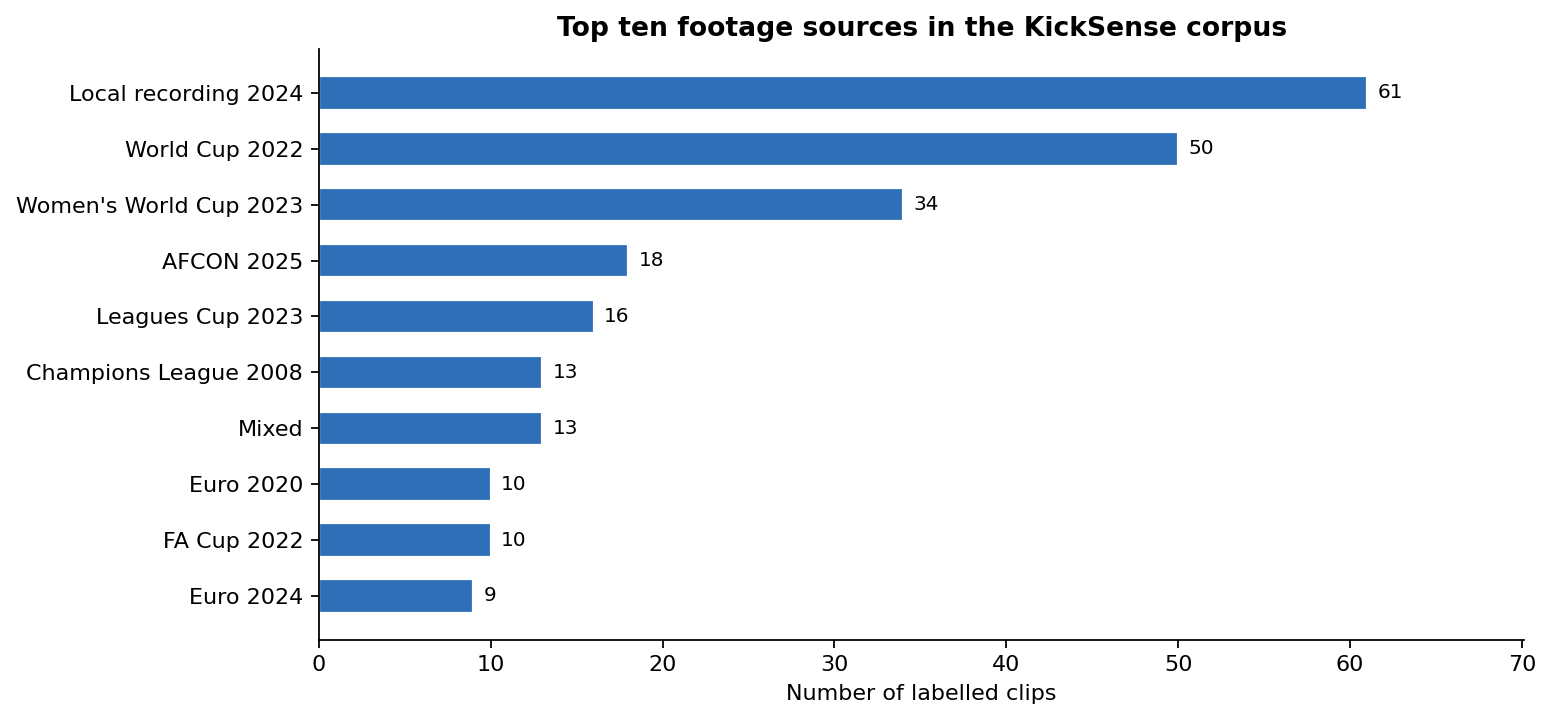
\includegraphics[width=0.92\textwidth]{fig17_source_distribution.png}
    \caption{Composition of the corpus by footage source}
    \label{fig:sources}
\end{figure}

\noindent
\textbf{Description:} The single largest contributor is the locally recorded session at 61 clips, followed by the men's World Cup 2022 at 50 and the Women's World Cup 2023 at 34, with the remainder distributed across fourteen further competitions. The spread across competitions is desirable because it varies players, stadiums, kit and broadcast style, which reduces the chance that the model latches onto a source specific artefact. The prominence of the local recordings is what makes the comparison in Section 4.5 possible.

\subsection{Temporal Footprint}

\begin{figure}[H]
    \centering
    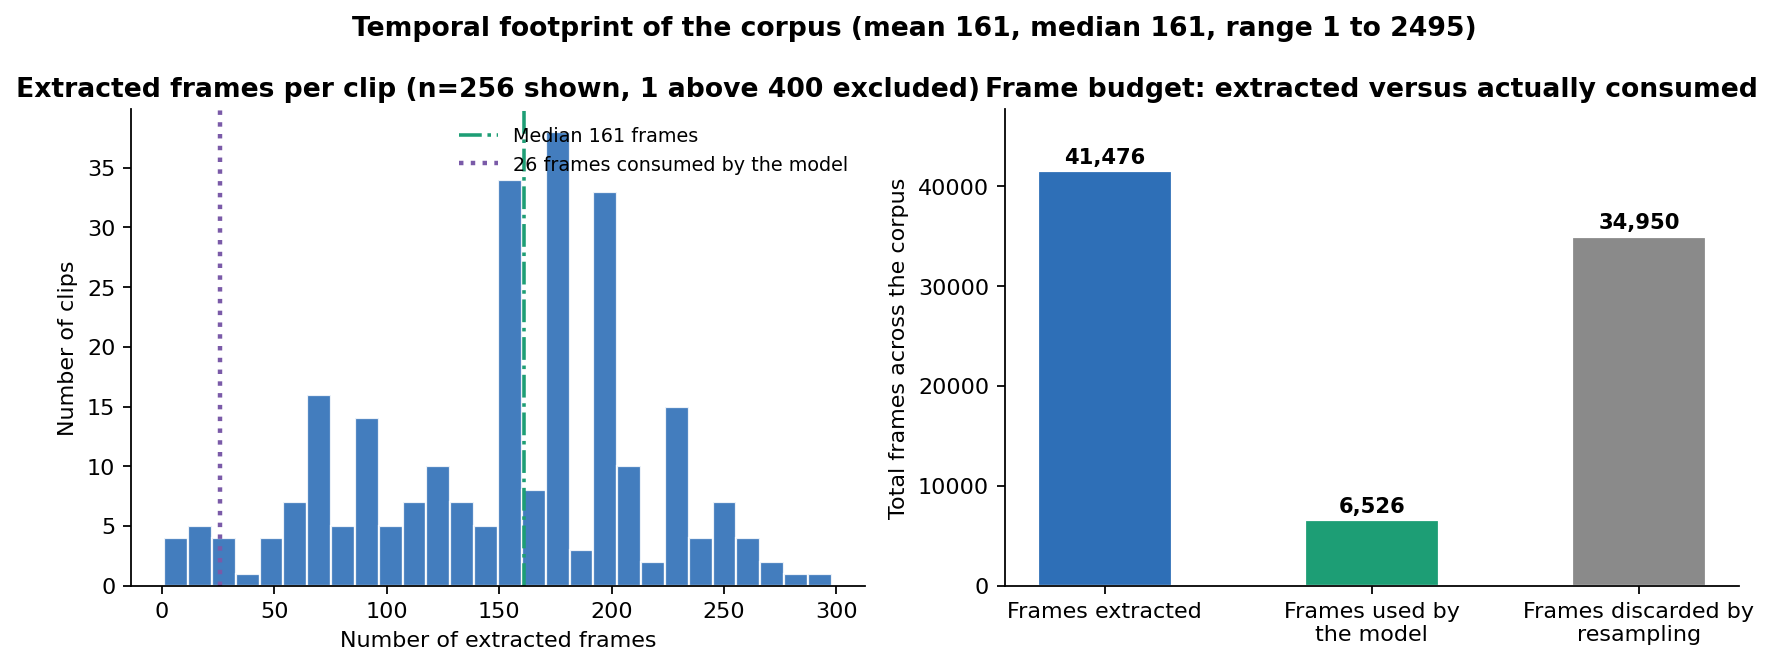
\includegraphics[width=0.99\textwidth]{fig13_frame_count_distribution.png}
    \caption{Frames extracted per clip and the proportion actually consumed by the model}
    \label{fig:frames}
\end{figure}

\noindent
\textbf{Description:} The left panel shows the distribution of extracted frames per clip, which is centred near the median of 161 frames with a long right tail. One clip contains 2,495 frames because the source video was not cut as tightly as the rest, and it is excluded from the histogram to keep the remaining distribution readable. A small number of clips contain fewer than twenty frames and are among those rejected by the quality gate. The right panel quantifies the frame budget explicitly: 41,476 frames were extracted and passed through pose estimation, of which 6,526 reach the model as time steps and 34,950 are discarded by the resampling step. This is the concrete answer to how many frames are extracted against how many are actually used.

\subsection{Feature Space and Normalisation}

The feature space is defined by the landmark topology shown in Figure \ref{fig:landmarks}. Each of the thirty three landmarks contributes four values, giving the one hundred and thirty two features per time step. Landmarks eleven, twelve, twenty three and twenty four additionally serve as the anchors that define the normalisation, since the hip midpoint provides the origin and the shoulder to hip distance provides the unit of length. This has a practical consequence for the dataset: a failure to detect the torso is far more damaging than a failure to detect an extremity, because without the anchors the entire frame cannot be normalised and the frame is lost even if most other landmarks were recovered successfully.

\section{Qualitative Experiments}

The qualitative evaluation asks whether the intermediate representation is visually faithful, in other words whether the skeleton the model receives genuinely corresponds to the player in the video. This matters more here than in a typical classification project, because the model never observes the image, so any systematic failure of the pose stage is invisible in the loss curve and will be silently absorbed as label noise.

\begin{figure}[H]
    \centering
    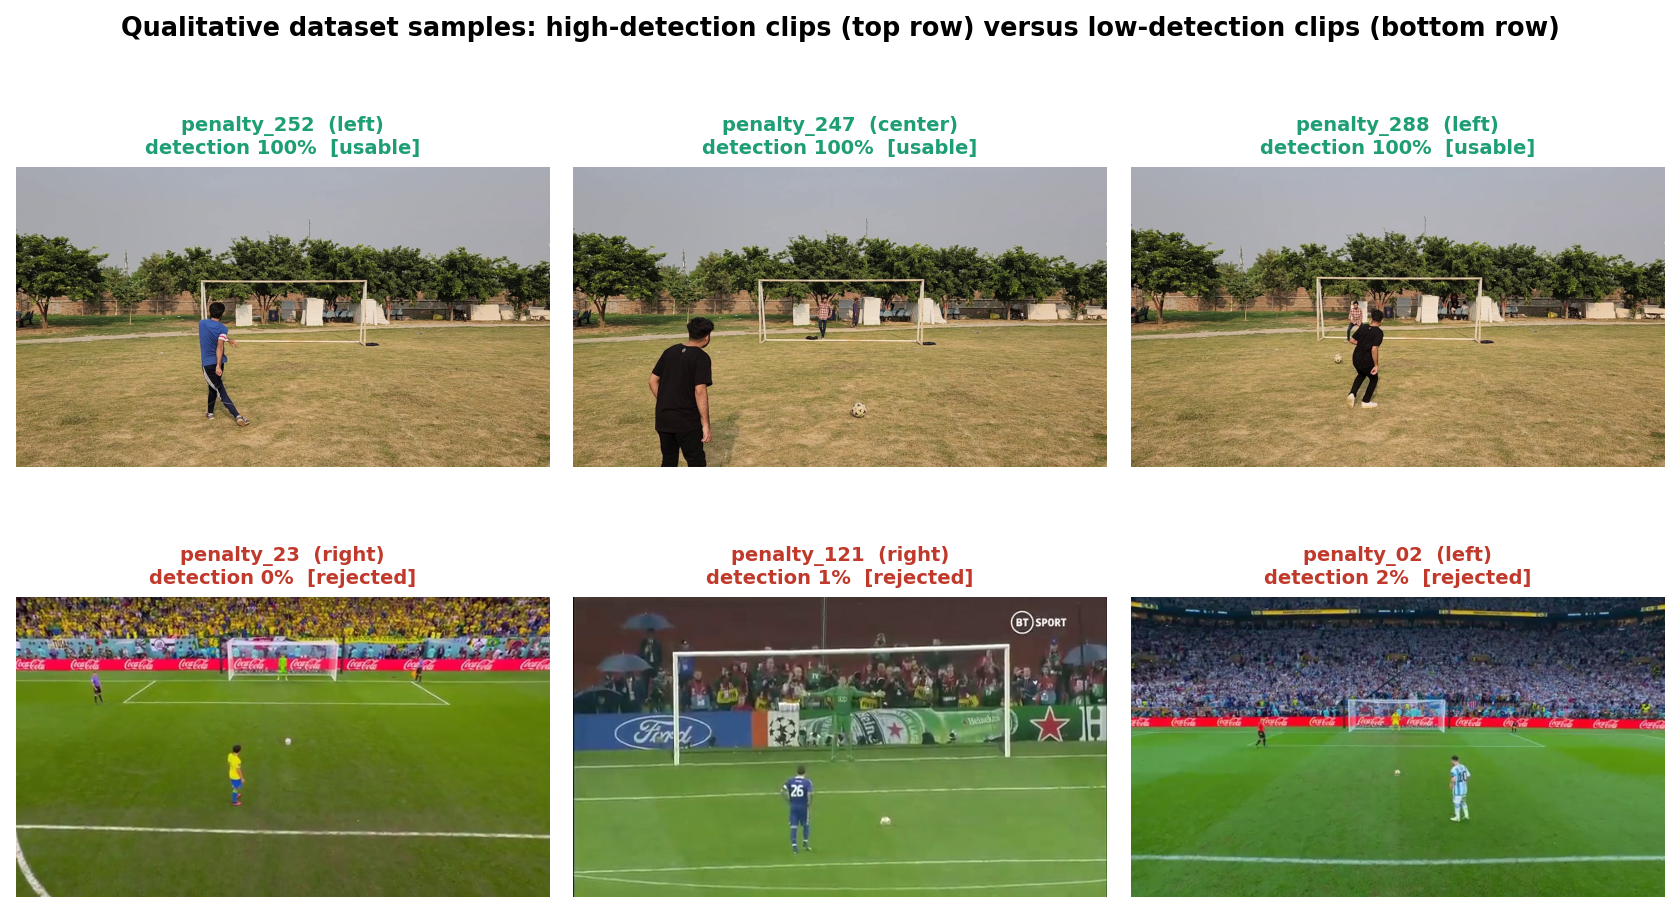
\includegraphics[width=0.99\textwidth]{fig25_qualitative_samples.png}
    \caption{Real frames from the highest and lowest pose detection clips in the corpus}
    \label{fig:qualitative}
\end{figure}

\noindent
\textbf{Description:} This montage is taken directly from the extracted frames and is the most revealing qualitative result in the project. The top row shows the three clips with the highest detection ratios, all at 100 percent, and all three are locally recorded clips in which the kicker occupies a large and unobstructed part of the frame. The bottom row shows the three lowest, at 0, 1 and 2 percent, and all three are broadcast clips filmed from an elevated wide angle in which the kicker occupies a small fraction of the image against a busy crowd background. The failure is therefore not random and not a defect of the pose estimator as such: it is a direct consequence of the subject's apparent size in the frame. This single observation explains the rejection rate reported in the next section and drives the corresponding future work.

The second qualitative check concerns whether the normalisation produces comparable representations, and the trajectory plots of Figure \ref{fig:trajectories} answer it. All three examples are centred near zero and expressed on the same scale despite originating from differently filmed clips, which confirms that the hip centring and torso scaling behave as intended. Equally important is what those trajectories do not show. The three classes do not separate cleanly, and the ankle trajectories of the left, centre and right examples overlap substantially. This is an honest visual preview of the moderate quantitative accuracy reported below, and it indicates that the discriminative signal is subtle rather than obvious, which is consistent with the fact that expert human goalkeepers also read penalties imperfectly.

The third qualitative check inspects a complete model input directly, as visualised in Figure \ref{fig:feature-tensor}. The structure of that tensor is coherent rather than noisy, with stable horizontal bands for landmarks that remain roughly fixed and strong temporal variation in the rows corresponding to the limbs involved in the kick. A tensor dominated by uniform noise would indicate a broken normalisation, so the visible structure is evidence that the representation carries organised temporal information for the convolutional and recurrent layers to exploit.

\section{Pose Detection Reliability}

\begin{figure}[H]
    \centering
    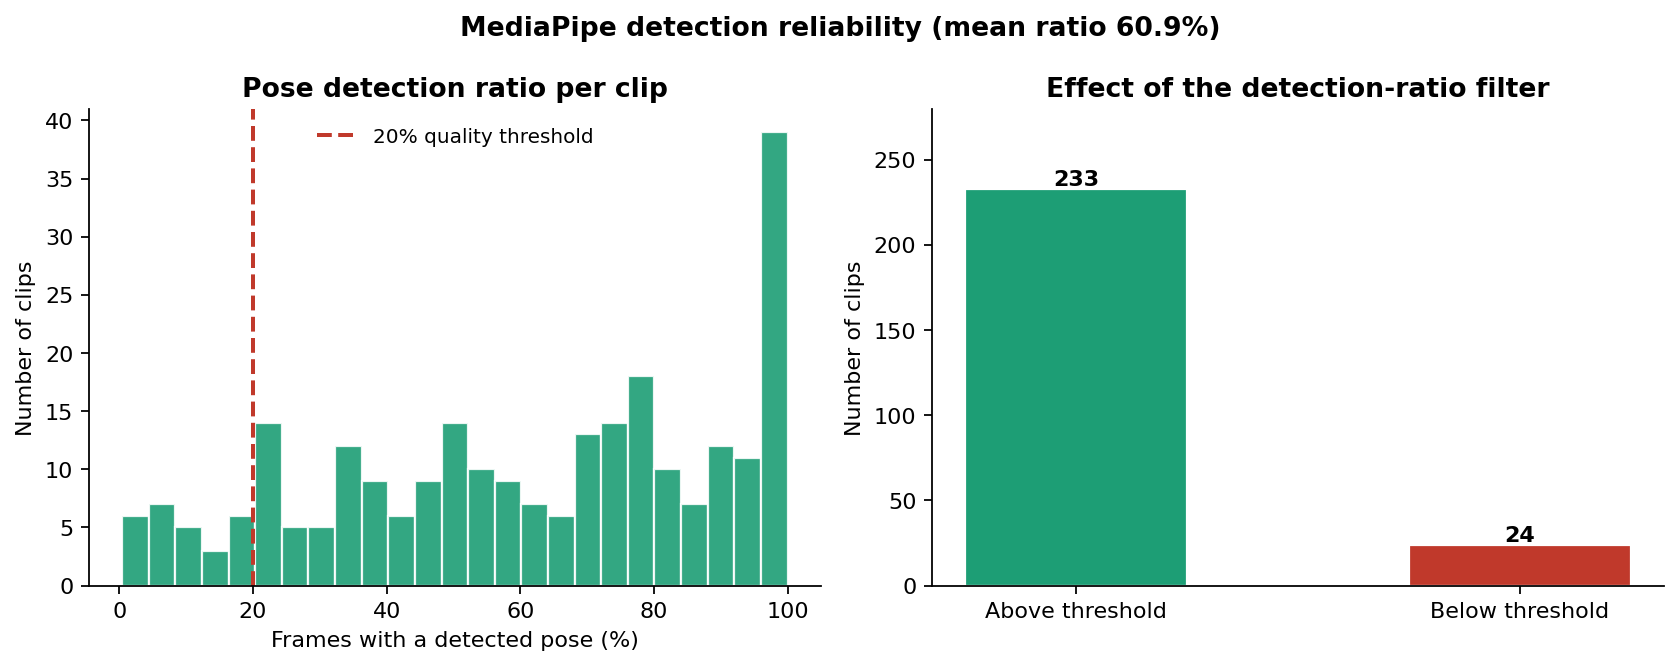
\includegraphics[width=0.99\textwidth]{fig14_detection_ratio.png}
    \caption{Pose detection ratio per clip and the effect of the 20 percent quality threshold}
    \label{fig:detection}
\end{figure}

\noindent
\textbf{Description:} Across 257 clips with a saved keypoint array, MediaPipe detected a pose in 60.9 percent of extracted frames on average, with a median of 66.0 percent. Thirty clips reached 100 percent detection and 24 clips fell below the 20 percent threshold and were therefore rejected. The distribution is broad rather than concentrated, which is itself the finding: pose extraction on this corpus is neither reliably successful nor reliably unsuccessful, but strongly dependent on how each individual clip was filmed.

Splitting the detection ratio by source makes the dependency explicit and quantifies the observation from the qualitative montage. Across the 61 locally recorded clips the mean detection ratio is 87.8 percent. Across the 195 broadcast clips it is 52.7 percent. The gap of thirty five percentage points is not a marginal effect, and it has a direct practical implication for the project: the cheapest available route to a larger and cleaner dataset is to record more footage locally rather than to source more broadcast penalties, because broadcast clips are both harder to obtain and roughly forty percent less likely to yield a usable pose stream per frame. This is why expanding the recorded corpus appears in the future work of Chapter 5.

\begin{figure}[H]
    \centering
    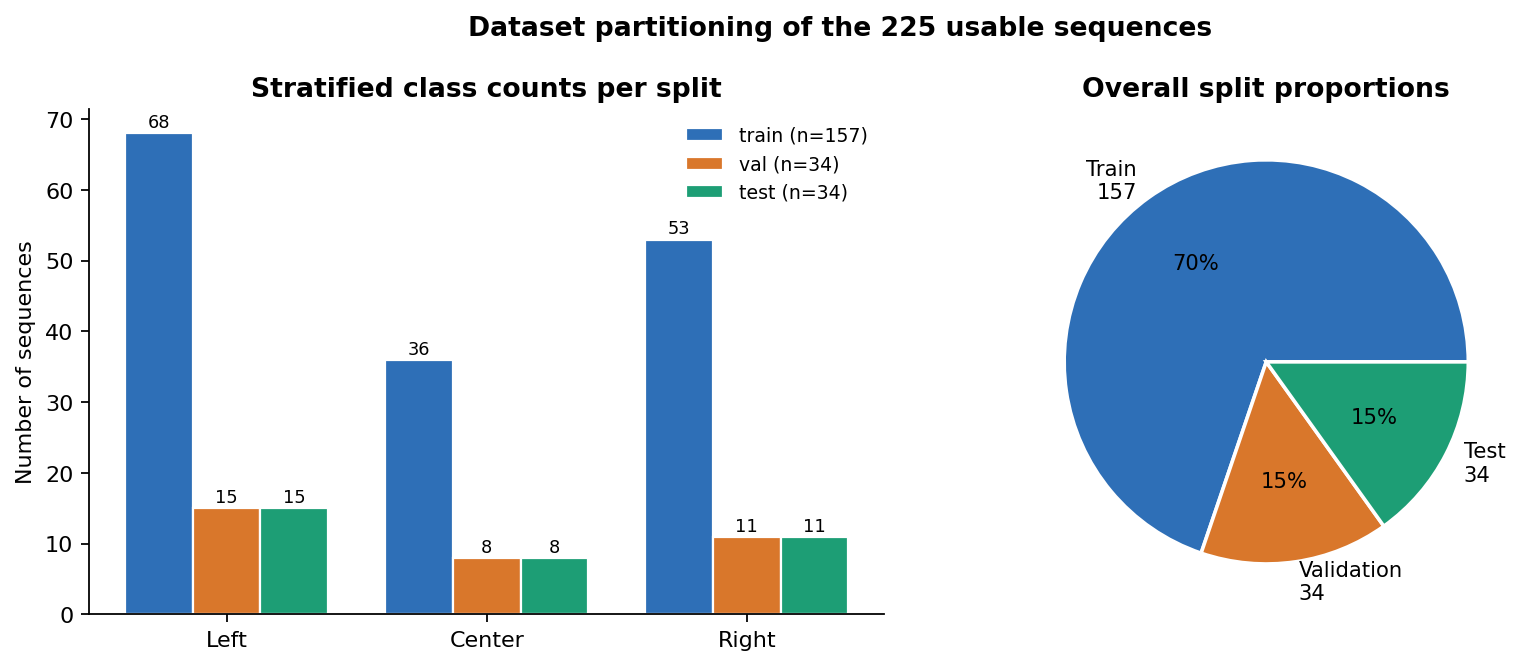
\includegraphics[width=0.99\textwidth]{fig15_split_distribution.png}
    \caption{Stratified partitioning of the 225 usable sequences}
    \label{fig:split}
\end{figure}

\noindent
\textbf{Description:} The stratified split preserves the class proportions in every partition. The training partition contains 68 left, 36 centre and 53 right sequences, and the validation and test partitions each contain 15 left, 8 centre and 11 right. The important consequence, and a limitation that must be kept in mind when reading every result in this chapter, is that with 34 test examples a single reclassified clip moves the reported accuracy by 2.9 percentage points. Differences smaller than about three points between configurations are therefore not meaningful, and this is stated here rather than glossed over because it governs how the ablation results should be interpreted.

\section{Quantitative Experiments}

\subsection{Evaluation Metrics and How They Are Validated}

The evaluation protocol is designed so that no information from the test partition influences the model in any way. The test set of 34 sequences is held out at the splitting stage, before any training occurs, and it is not used for early stopping, for checkpoint selection or for any hyperparameter decision. Early stopping monitors validation direction accuracy and restores the weights of the best validation epoch, so the validation set is consumed by model selection and its accuracy is consequently optimistic. The test accuracy is measured exactly once per configuration on the restored checkpoint. This separation is why the validation and test figures reported below differ, and why only the test figures should be read as estimates of generalisation.

\renewcommand{\arraystretch}{1.25}
\small
\begin{longtable}{|>{\bfseries}p{3.0cm}|p{4.4cm}|p{6.2cm}|}
\hline
\textbf{Metric} & \textbf{Definition} & \textbf{Why it is used here} \\ \hline
\endfirsthead
\hline
\textbf{Metric} & \textbf{Definition} & \textbf{Why it is used here} \\ \hline
\endhead
\hline
\multicolumn{3}{r}{\textit{Continued on next page}} \\
\hline
\endfoot
\hline
\endlastfoot
Accuracy & Correct predictions divided by total predictions & Primary headline metric, directly interpretable against the 33.3 percent random baseline \\ \hline
Precision & True positives over predicted positives, per class and weighted & Reveals whether a class is predicted too liberally \\ \hline
Recall & True positives over actual positives, per class and weighted & Reveals whether a class is being missed, which is the failure mode of the minority class \\ \hline
F1-score & Harmonic mean of precision and recall & Single summary per class that neither precision nor recall gives alone \\ \hline
Confusion matrix & Full three by three table of actual against predicted & Shows which specific classes are confused with which, not merely how often \\ \hline
MAE & Mean absolute error of the power prediction & Directly interpretable as an average error in points on the one to ten scale \\ \hline
MSE and RMSE & Mean squared error and its root & Penalise large power errors more heavily than MAE, exposing outliers \\ \hline
\caption{Evaluation metrics used and the reason each is reported}
\label{tab:metrics}
\end{longtable}
\normalsize

\noindent
\textbf{Description:} All classification metrics are computed with scikit-learn using weighted averaging for the aggregate figures, so that each class contributes in proportion to its support, and with division by zero handled explicitly so that an unpredicted class produces a score of zero rather than an undefined value. The weighted average is preferred over the macro average here because the class imbalance is a genuine property of the sport rather than a sampling artefact, so a metric that reflects the real class proportions is the more honest summary.

It is worth stating why these particular metrics are used rather than those a segmentation task would report. Mean intersection over union, the standard metric for semantic segmentation, measures the spatial overlap between a predicted region and a ground truth region. KickSense produces no spatial region: its direction output is a categorical choice among three classes and its power output is a scalar. There is nothing to intersect, so the intersection over union family is not merely unnecessary here but undefined. The classification and regression metrics above are the correct analogues, and the confusion matrix plays the diagnostic role for this task that a per class intersection over union table plays for segmentation.

\subsection{Reference Model Results}

All test set numbers in this subsection come from a single checkpoint, namely the full configuration trained with a fixed seed of forty two, which stopped at epoch 28 after early stopping restored the weights from its best validation epoch. Using one checkpoint for all of them ensures the confusion matrix, the per class metrics and the power regression plots describe the same model rather than a mixture of runs.

\begin{figure}[H]
    \centering
    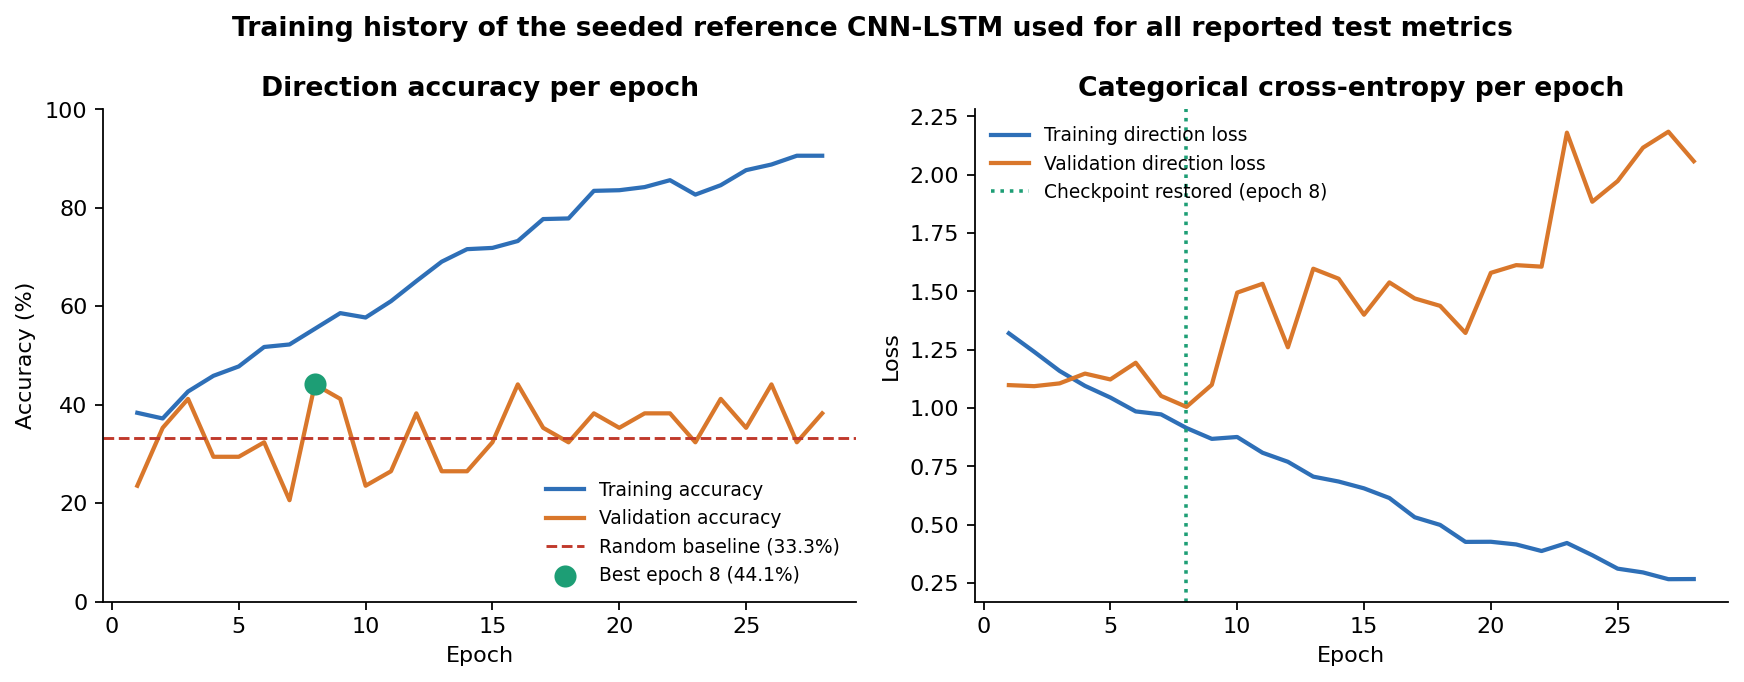
\includegraphics[width=0.99\textwidth]{fig18_training_curves.png}
    \caption{Training history of the seeded reference model}
    \label{fig:training}
\end{figure}

\noindent
\textbf{Description:} The left panel shows that training accuracy rises steadily and passes eighty percent while validation accuracy plateaus in the mid forties, which is the signature of overfitting on a small dataset and is precisely what the regularisation stack is intended to slow rather than eliminate. The right panel shows the corresponding cross entropy curves, with the validation loss flattening while the training loss continues to fall. Early stopping halts training at epoch 28 and restores the best validation epoch, so the divergence visible at the right hand edge of both panels is observed but not inherited by the evaluated model.

\renewcommand{\arraystretch}{1.3}
\small
\begin{longtable}{|>{\bfseries}p{6.0cm}|p{3.4cm}|p{4.0cm}|}
\hline
\textbf{Result} & \textbf{Value} & \textbf{Reference point} \\ \hline
\endfirsthead
\hline
\textbf{Result} & \textbf{Value} & \textbf{Reference point} \\ \hline
\endhead
\hline
\multicolumn{3}{r}{\textit{Continued on next page}} \\
\hline
\endfoot
\hline
\endlastfoot
Test set size & 34 sequences & 15 left, 8 centre, 11 right \\ \hline
Direction accuracy & 44.1 percent & Random baseline 33.3 percent \\ \hline
Weighted precision & 50.0 percent & \\ \hline
Weighted recall & 44.1 percent & Equal to accuracy by definition \\ \hline
Weighted F1-score & 41.4 percent & \\ \hline
Best validation accuracy, this run & 44.1 percent & Reached at epoch 8 \\ \hline
Best validation accuracy, any run & 55.9 percent & Epoch 29 of the visual label run \\ \hline
Best test accuracy, any logged run & 48.0 percent & Recorded in the first retrain log \\ \hline
Power MAE & 2.99 points & On the 1 to 10 scale \\ \hline
Power RMSE & 3.38 points & \\ \hline
Epochs to early stop & 28 & Patience 20 on validation accuracy \\ \hline
Trainable parameters & 248,580 & 249,220 including BN statistics \\ \hline
Augmented training sequences & 785 & From 157 originals \\ \hline
\caption{Quantitative results of the reference model on the held out test set}
\label{tab:test-results}
\end{longtable}
\normalsize

\noindent
\textbf{Description:} The headline result is 44.1 percent test direction accuracy against a 33.3 percent random baseline, which is a relative improvement of roughly a third over chance. Three separate accuracy figures are reported deliberately rather than only the most flattering one. The 44.1 percent is the reproducible test accuracy of the seeded reference model and is the figure that should be quoted as the current result. The 55.9 percent is the highest validation accuracy recorded anywhere in the project and is reported because it is a real measurement, but it is a validation figure and therefore optimistic. The 48.0 percent is the highest test accuracy recorded in any saved log. The spread between these numbers is itself a finding, discussed in Section 4.8.

\begin{figure}[H]
    \centering
    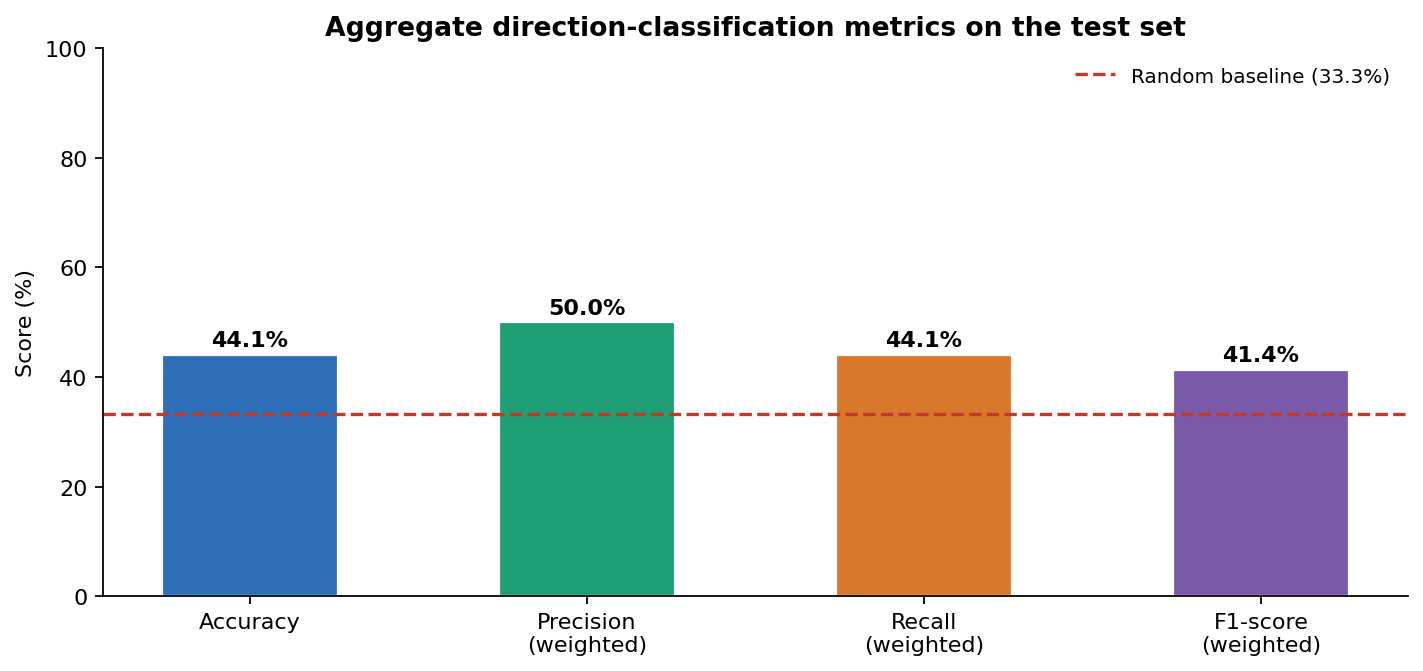
\includegraphics[width=0.99\textwidth]{fig21_metrics_overview.png}
    \caption{Aggregate direction classification metrics against the random baseline}
    \label{fig:metrics}
\end{figure}

\noindent
\textbf{Description:} All four aggregate metrics sit clearly above the 33.3 percent random baseline, which establishes that the model has learned a genuine signal rather than a class prior. The weighted precision of 50.0 percent exceeds the recall of 44.1 percent, which indicates the model is conservative in a specific way: when it commits to a class it is right half the time, but it fails to recover a majority of the true instances of at least one class. The confusion matrix identifies which.

\begin{figure}[H]
    \centering
    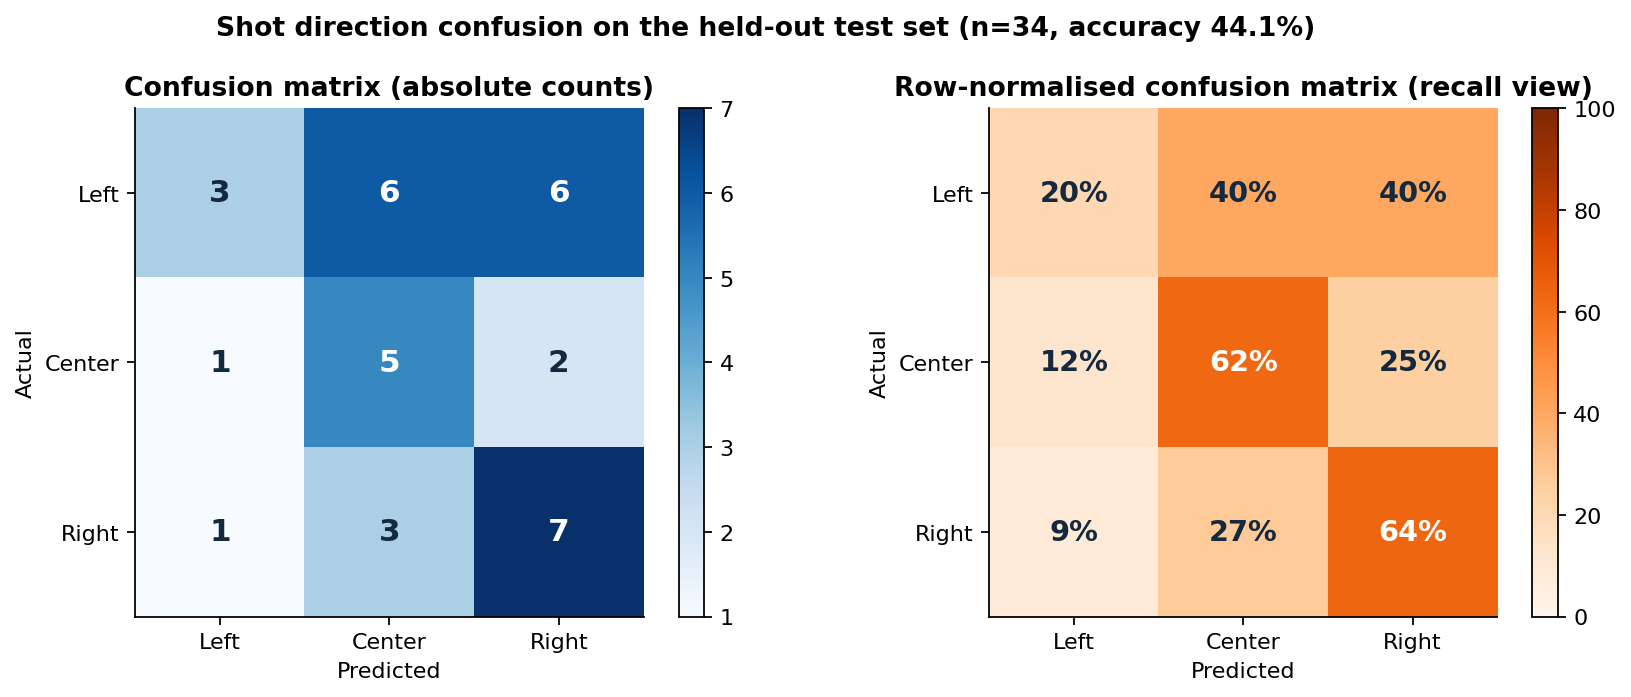
\includegraphics[width=0.99\textwidth]{fig19_confusion_matrix.png}
    \caption{Confusion matrix on the held out test set, in absolute counts and row normalised form}
    \label{fig:confusion}
\end{figure}

\noindent
\textbf{Description:} The confusion matrix is the most diagnostic result in the chapter. Reading the rows, the left class is recovered in only 3 of 15 cases, with 6 misclassified as centre and 6 as right. The centre class is recovered in 5 of 8 cases and the right class in 7 of 11. The pattern is therefore not a uniform difficulty but a specific and asymmetric failure: the model systematically under predicts left shots and disperses them across the other two classes, while handling right and centre comparatively well. This is a more useful finding than the accuracy figure alone, because it points at a concrete cause. The mirror augmentation converts every left example into a right example and vice versa, so after augmentation the left and right classes are numerically balanced; if the underlying left examples are visually harder, for instance because more of them come from broadcast clips filmed from an angle that foreshortens the run up, then balance in count does not translate into balance in learnability. Investigating this asymmetry is a concrete next step rather than a general aspiration.

\begin{figure}[H]
    \centering
    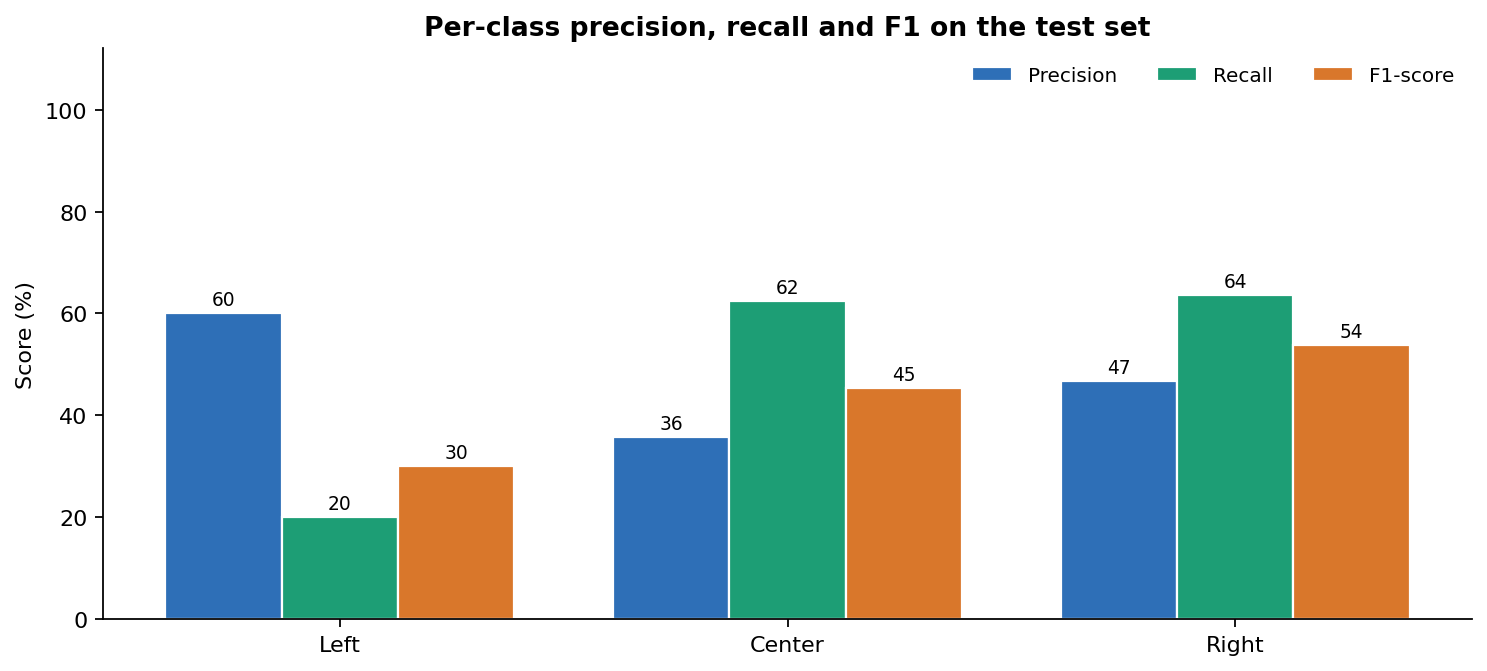
\includegraphics[width=0.92\textwidth]{fig20_per_class_metrics.png}
    \caption{Per class precision, recall and F1 score on the test set}
    \label{fig:per-class}
\end{figure}

\noindent
\textbf{Description:} The per class breakdown quantifies the asymmetry the confusion matrix exposes. The left class attains 60.0 percent precision but only 20.0 percent recall, giving an F1 of 30.0 percent, which is the profile of a class the model predicts rarely but with reasonable reliability when it does. The centre class attains 35.7 percent precision with 62.5 percent recall and an F1 of 45.5 percent, the opposite profile of a class the model over predicts. The right class is the most balanced at 46.7 percent precision, 63.6 percent recall and 53.8 percent F1. Notably, the centre class is not the weakest despite having the least support, which suggests the class weighting is doing its job and that support alone does not determine per class performance here.

\begin{figure}[H]
    \centering
    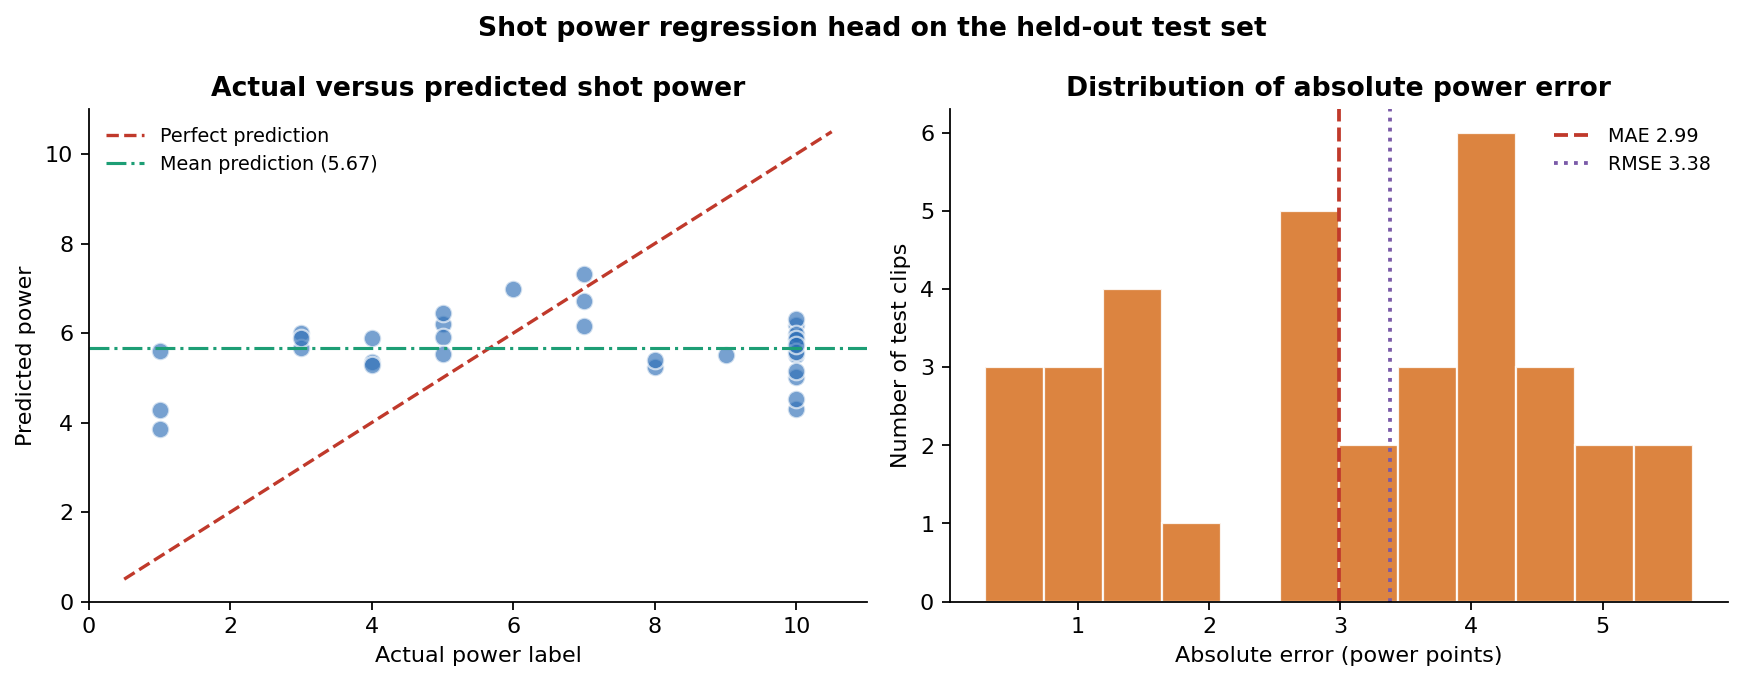
\includegraphics[width=0.99\textwidth]{fig22_power_regression.png}
    \caption{Shot power regression behaviour on the test set}
    \label{fig:power-reg}
\end{figure}

\noindent
\textbf{Description:} The power head performs poorly, and the left panel shows why in a way the error metric alone does not. The predictions cluster in a narrow horizontal band rather than following the diagonal, which means the model is largely predicting a value close to the training mean regardless of the input. The mean absolute error of 2.99 points on a one to ten scale should therefore be read as evidence that the power head has not learned a useful mapping rather than as evidence of moderate accuracy. The cause is diagnosable from Section 4.2: the power labels are strongly bimodal with 76 clips at ten and 40 at one, so the target is closer to a coarse category than a graded measurement, and predicting the mean is close to the optimal strategy under mean squared error for a target the input cannot explain. Replacing the subjective scale with a measurement derived from frame to frame ball displacement is consequently the highest value item in the future work of Chapter 5, and the honest statement of the current position is that direction prediction works above chance while power prediction does not yet work.

\section{Ablation Study}

The ablation study trains six configurations under identical conditions with the same seed and the same split, each differing from the full model by exactly one factor. Its purpose is to determine which design decisions contribute to the result, which is a question the development history cannot answer because those runs differed in several respects at once.

\begin{figure}[H]
    \centering
    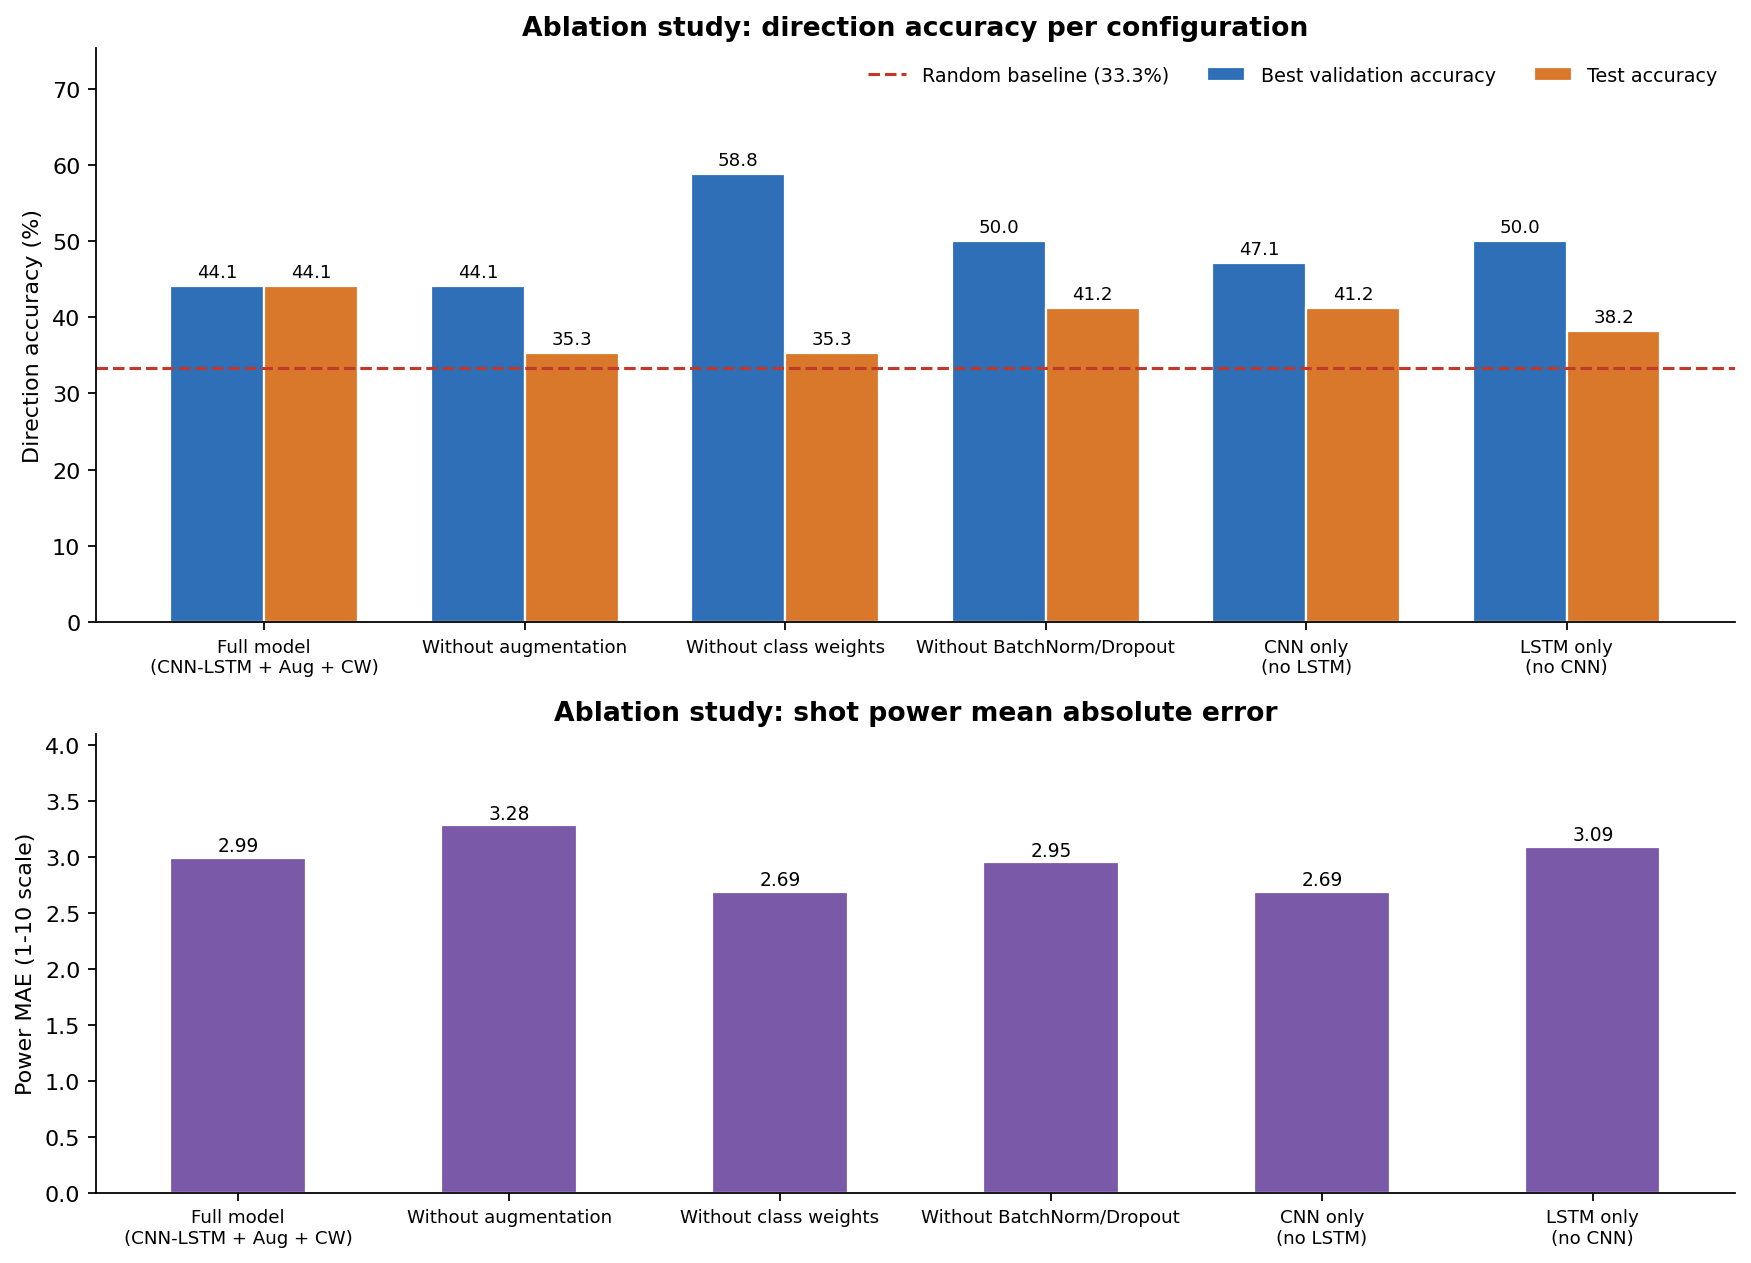
\includegraphics[width=0.99\textwidth]{fig23_ablation_study.png}
    \caption{Ablation study over architecture, augmentation, class weighting and regularisation}
    \label{fig:ablation}
\end{figure}

\noindent
\textbf{Description:} The upper panel reports the best validation accuracy and the test accuracy of each configuration and the lower panel reports the power mean absolute error. The full model attains the highest test accuracy of all six configurations, and every ablated variant is worse on the test set, which supports the architecture as a whole. The validation figures do not rank the configurations in the same order as the test figures, which is discussed below and is a finding in its own right.

\begin{table}[H]
\centering
\renewcommand{\arraystretch}{1.3}
\setlength{\tabcolsep}{4pt}
\small
\begin{tabular}{|>{\raggedright\arraybackslash\bfseries}p{4.0cm}|r|r|r|r|r|}
\hline
\textbf{Configuration} & \textbf{Params} & \textbf{Epochs} & \textbf{Val. acc.} & \textbf{Test acc.} & \textbf{MAE} \\ \hline
Full model (CNN-LSTM, augmentation, class weights) & 249,220 & 28 & 44.1\% & \textbf{44.1\%} & 2.99 \\ \hline
Without augmentation & 249,220 & 21 & 44.1\% & 35.3\% & 3.28 \\ \hline
Without class weights & 249,220 & 63 & \textbf{58.8\%} & 35.3\% & \textbf{2.69} \\ \hline
Without BatchNorm and Dropout & 247,940 & 35 & 50.0\% & 41.2\% & 2.95 \\ \hline
CNN only, no LSTM & 76,420 & 46 & 47.1\% & 41.2\% & 2.69 \\ \hline
LSTM only, no CNN & 200,388 & 46 & 50.0\% & 38.2\% & 3.09 \\ \hline
Random baseline & n/a & n/a & 33.3\% & 33.3\% & n/a \\ \hline
\end{tabular}
\caption{Ablation results, all configurations trained with seed 42 on the identical split}
\label{tab:ablation}
\end{table}
\normalsize
\setlength{\tabcolsep}{6pt}

\noindent
\textbf{Description:} Reading the test accuracy column, the full model at 44.1 percent leads, followed by the two variants at 41.2 percent, the recurrent only variant at 38.2 percent, and the two weakest at 35.3 percent. The power mean absolute error column shows much less variation, between 2.69 and 3.28, which is consistent with the finding of Section 4.6 that no configuration has learned a useful power mapping.

Four conclusions follow, and they are stated with the precision the test set size permits.

The clearest result is that \textbf{augmentation matters}. Removing it drops test accuracy from 44.1 to 35.3 percent, a gap of 8.8 percentage points corresponding to three test clips, and it also produces the worst power error of any configuration at 3.28. It additionally stops training earliest, at 21 epochs, which is the expected consequence of training on 157 rather than 785 sequences. This is the only individual effect in the table large enough to sit comfortably outside the roughly three point noise floor established in Section 4.5.

The second result is that \textbf{both halves of the encoder contribute}. Removing the recurrent layers costs 2.9 points of test accuracy and removing the convolutional layers costs 5.9 points, so neither component is redundant and the hybrid outperforms either alone. The convolution only variant is the more interesting of the two, because it reaches 41.2 percent with 76,420 parameters, less than a third of the full model. Given the dataset size this is worth noting explicitly: a substantially smaller model is nearly as accurate, which suggests the full model's capacity is not the limiting factor and that data, not architecture, is the binding constraint.

The third result concerns \textbf{class weighting}, and it is the most instructive because it is counterintuitive. Removing class weighting produces the highest validation accuracy in the entire table, at 58.8 percent, while simultaneously producing one of the lowest test accuracies, at 35.3 percent. Two things follow. First, this configuration is the one that matches the production training script, since as noted in Chapter 3 that script computes class weights but cannot pass them to a multi output Keras model, which explains why the 55.9 percent validation figure recorded in the project logs is consistent with the 58.8 percent observed here. Second, and more importantly, a 23 point gap between validation and test accuracy in the same run demonstrates that with 34 validation examples the validation set is too small to select models reliably. This is a genuine methodological weakness of the current protocol and it is the reason that stratified k fold cross validation, rather than a single held out validation split, is listed as future work.

The fourth result is that \textbf{removing regularisation is not catastrophic}, costing 2.9 points of test accuracy, which is within the noise floor. The regularisation stack should therefore be understood as a reasonable precaution whose benefit is not individually measurable at this dataset size rather than as a demonstrated necessity.

\section{Development History}

\begin{figure}[H]
    \centering
    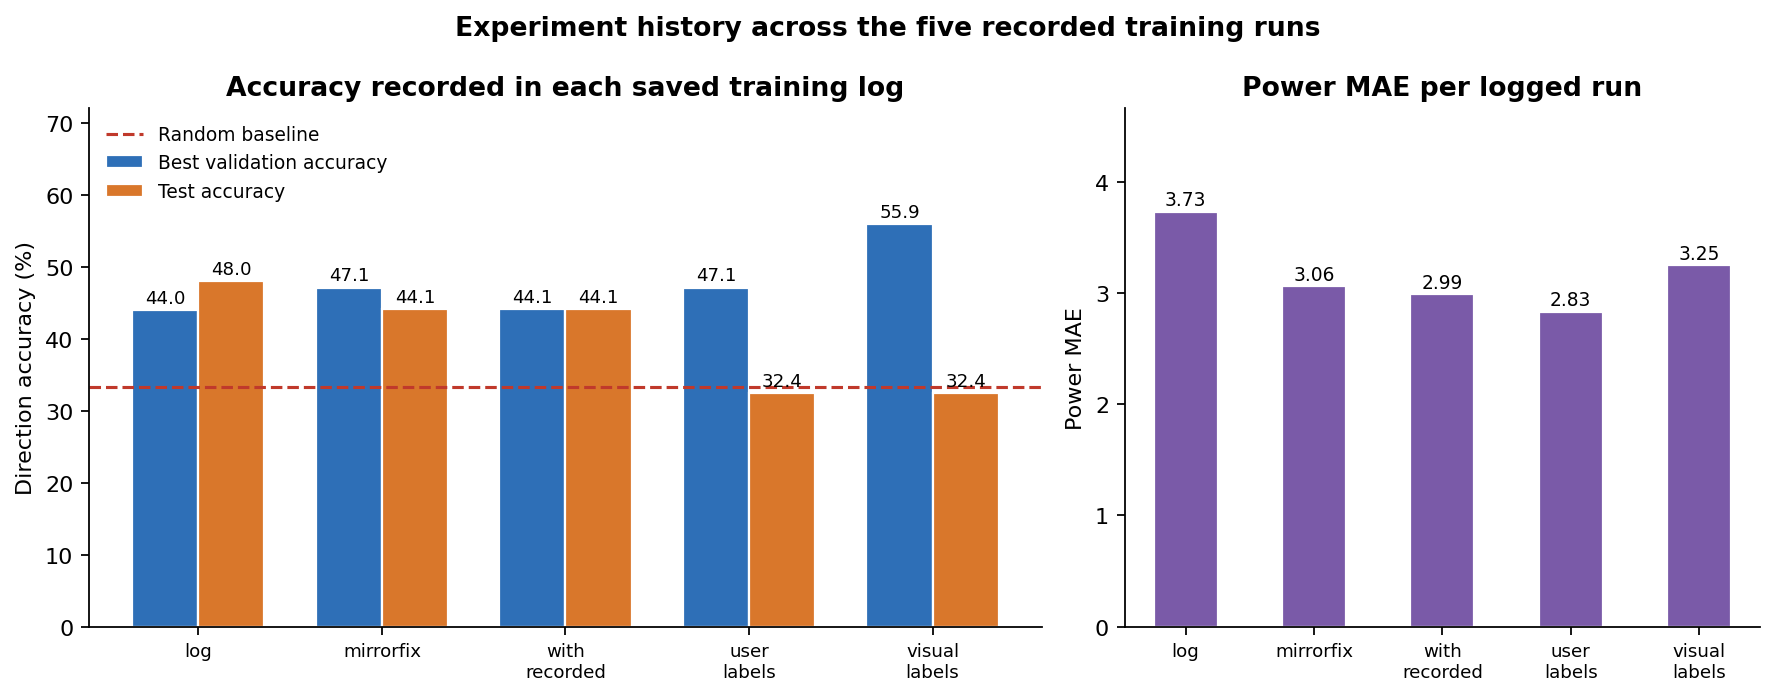
\includegraphics[width=0.99\textwidth]{fig24_run_comparison.png}
    \caption{Accuracy and power error recorded across the five saved training runs}
    \label{fig:runs}
\end{figure}

\noindent
\textbf{Description:} These five runs are the preserved development history, and unlike the ablation they differ from one another in the state of the data as well as the code, so they document progress rather than support attribution. Validation accuracy improves across the sequence from 44.0 to 55.9 percent as the corpus grew with locally recorded footage, a defect in the mirror augmentation was corrected, and a portion of the direction labels was re-verified against the video. Test accuracy does not follow the same trend, which is the same instability the ablation exposed.

\begin{figure}[H]
    \centering
    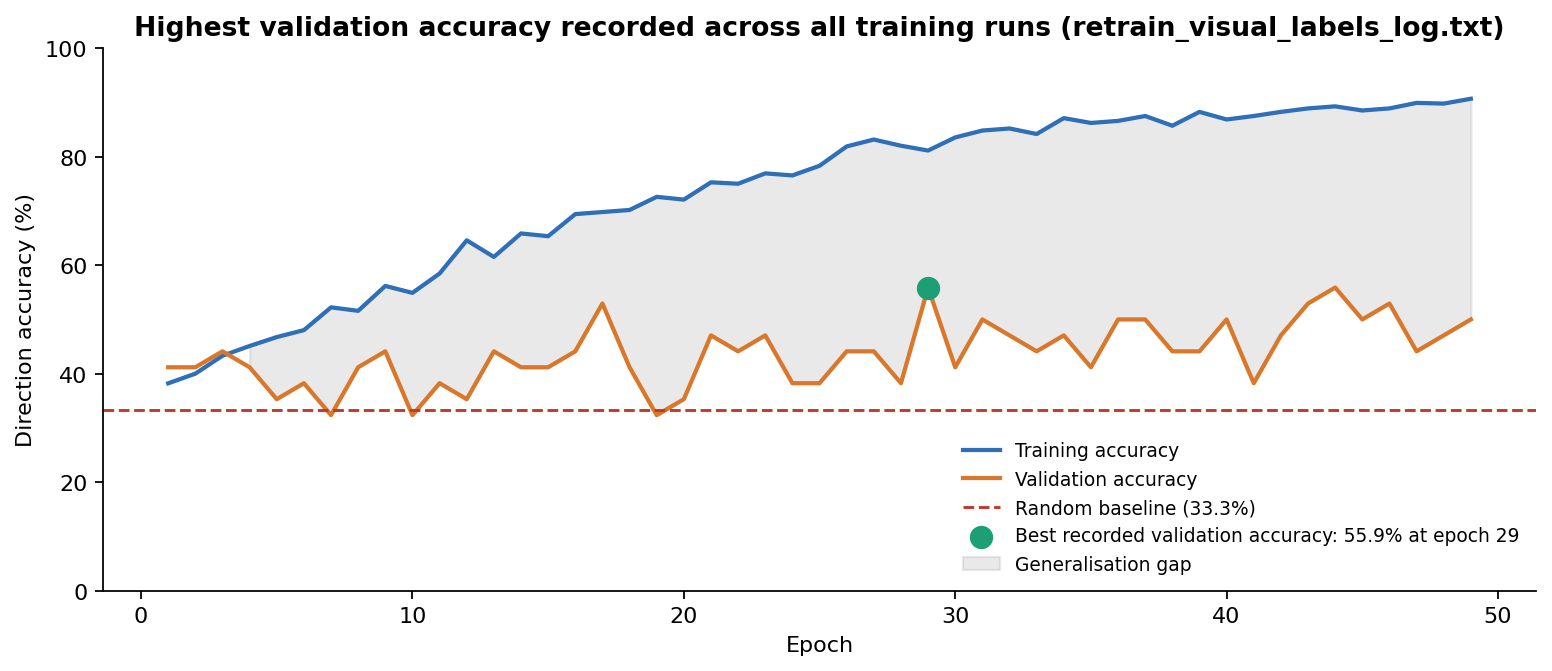
\includegraphics[width=0.99\textwidth]{fig28_historical_best_run.png}
    \caption{The training run that produced the highest validation accuracy recorded in the project}
    \label{fig:historical}
\end{figure}

\noindent
\textbf{Description:} This figure shows the full 49 epoch history of the run that reached 55.9 percent validation direction accuracy at epoch 29, the highest figure recorded anywhere in the project. The shaded region marks the generalisation gap between training and validation accuracy, which widens steadily as training progresses and is the visual signature of the small dataset problem. The run is presented here because it is a genuine logged measurement, but the reference model of Section 4.6 rather than this run is the basis for every test set number in this chapter, because this checkpoint was subsequently overwritten by later retraining and cannot be re-evaluated.

\begin{table}[H]
\centering
\renewcommand{\arraystretch}{1.3}
\setlength{\tabcolsep}{4pt}
\small
\begin{tabular}{|>{\raggedright\arraybackslash\bfseries}p{3.4cm}|r|r|r|>{\raggedright\arraybackslash}p{4.0cm}|}
\hline
\textbf{Saved log} & \textbf{Val. acc.} & \textbf{Test acc.} & \textbf{MAE} & \textbf{Change in that run} \\ \hline
retrain & 44.0\% & 48.0\% & 3.73 & Baseline, 114 training samples \\ \hline
with\_recorded & 44.1\% & 44.1\% & 2.99 & Locally recorded clips added \\ \hline
mirrorfix & 47.1\% & 44.1\% & 3.06 & Mirror augmentation defect corrected \\ \hline
user\_labels & 47.1\% & 32.4\% & 2.83 & Direction labels revised \\ \hline
visual\_labels & \textbf{55.9\%} & 32.4\% & 3.25 & Labels re-verified against footage \\ \hline
\end{tabular}
\caption{The five recorded training runs and the change introduced in each. Log file names are abbreviated from \texttt{retrain\_*\_log.txt} in \texttt{outputs/model}}
\label{tab:run-history}
\end{table}
\normalsize
\setlength{\tabcolsep}{6pt}

\noindent
\textbf{Description:} This table records the development history honestly, including the fact that the two runs with the highest validation accuracy have the lowest test accuracy. Presented alone either column would be misleading. Presented together they show that improvements which appeared real when measured on 34 validation examples did not transfer to the test partition, and this is the single strongest piece of evidence that the evaluation protocol, rather than the model, is the immediate bottleneck in the project.

\section{Comparison with the Base Paper}

The base paper of Salazar and Alatrista-Salas addresses the same prediction task with the same three way regional formulation \cite{salazar2024}, so a comparison is natural. It is nonetheless not possible to make a numerical one, and the reason must be stated plainly rather than worked around. Both projects had to construct a bespoke corpus because no public dataset annotates penalty direction, and the base paper's corpus is not publicly released. The two datasets therefore differ in size, in the competitions they draw from, in camera angles, and in annotation schema. An accuracy figure obtained on one corpus and an accuracy figure obtained on the other measure the difficulty of two different datasets at least as much as they measure the quality of two different models, so placing them side by side and declaring a winner would be a claim the evidence cannot support. No such claim is made in this report.

What can be compared is methodology, computational cost, output scope and evaluation rigour, and Table \ref{tab:metric-compare} does so.

\renewcommand{\arraystretch}{1.3}
\small
\begin{longtable}{|>{\raggedright\arraybackslash\bfseries}p{3.4cm}|>{\raggedright\arraybackslash}p{4.9cm}|>{\raggedright\arraybackslash}p{4.9cm}|}
\hline
\textbf{Aspect} & \textbf{Salazar and Alatrista-Salas (2024)} & \textbf{KickSense} \\ \hline
\endfirsthead
\hline
\textbf{Aspect} & \textbf{Salazar and Alatrista-Salas (2024)} & \textbf{KickSense} \\ \hline
\endhead
\hline
\multicolumn{3}{r}{\textit{Continued on next page}} \\
\hline
\endfoot
\hline
\endlastfoot
Evaluation dataset & Bespoke corpus, not publicly released & Bespoke corpus of 225 usable sequences, fully documented in this repository \\ \hline
Metrics reported & Accuracy of regional prediction, plus a study of body part influence & Accuracy, weighted and per class precision, recall and F1, confusion matrix, MAE, MSE and RMSE \\ \hline
Reason the metrics differ & Single classification output, so accuracy plus interpretability analysis suffices & Two heads require both classification and regression metrics; per class metrics are necessary because the classes are unbalanced \\ \hline
Random baseline stated & Not emphasised & Stated explicitly as 33.3 percent alongside every accuracy figure \\ \hline
Test protocol & Not fully specified in the published description & Held out 34 sequence test split, never used for early stopping or model selection, evaluated once per configuration \\ \hline
Pose stage cost & TAM segmentation and MMPose 3D pose, requires a graphics processor & MediaPipe Pose on CPU, runs on a consumer laptop \\ \hline
Output scope & Goal region only & Goal region plus a shot power estimate \\ \hline
Ablation analysis & Three model families compared & Six configurations varying architecture, augmentation, class weighting and regularisation, all under one seed and split \\ \hline
Direct accuracy comparison & \multicolumn{2}{|>{\raggedright\arraybackslash}p{10.3cm}|}{Not performed. The corpora differ and neither is available to the other, so any head to head accuracy claim would be unsupported.} \\ \hline
\caption{Comparison of the evaluation protocols of the base paper and KickSense}
\label{tab:metric-compare}
\end{longtable}
\normalsize

\noindent
\textbf{Description:} The comparison is deliberately restricted to what the available evidence supports. KickSense reports a broader metric set on a documented and reproducible split, and it delivers an additional output that the base paper does not attempt, at a computational cost low enough for consumer hardware. It does not claim higher accuracy, because the datasets differ. The one point on which KickSense is unambiguously ahead is reproducibility, since every figure and every number in this chapter can be regenerated from the repository, which is not true of a result reported on an unreleased corpus.

\section{Summary of Findings}

The evaluation supports five conclusions. First, the direction prediction works above chance, at 44.1 percent test accuracy against a 33.3 percent baseline, and this is a real if modest result. Second, the power prediction does not yet work, since the head largely predicts the training mean, and the diagnosis points at the bimodal subjective annotation rather than at the architecture. Third, the pose stage is the dominant data quality bottleneck, with an average detection ratio of 87.8 percent on locally recorded clips against 52.7 percent on broadcast clips, which makes local recording the most efficient route to a better dataset. Fourth, augmentation is the only training component whose individual contribution is measurable above the noise floor, and both halves of the hybrid encoder contribute while a model a third of the size is nearly as accurate, which together indicate that data rather than model capacity is the binding constraint. Fifth, and most consequentially for the next phase of the project, a 34 example validation set is too small for reliable model selection, as demonstrated by a 23 point validation to test gap within a single run, which makes cross validation the highest priority methodological fix.

\clearpage


\chapter{Conclusion}
\section{Summary of Work Completed}

KickSense set out to determine whether the directional and power intent of a football penalty kick can be predicted from the kicker's body motion alone, using ordinary single camera video and consumer hardware. The work completed to date establishes that the answer for direction is yes, at a level meaningfully above chance, and that the answer for power is not yet, for reasons that are diagnosed rather than merely observed.

The concrete deliverables are as follows. A corpus of three hundred and one penalty kick videos was collected from seventeen competitions and from dedicated local recording sessions, and two hundred and fifty nine of these clips were manually annotated with shot direction, shot power, outcome, ball placement, dominant foot, match and tournament in a single authoritative spreadsheet. Every clip was decoded to frames, giving forty one thousand four hundred and seventy six frames in total, and every frame was passed through MediaPipe Pose at model complexity two, yielding a pose in twenty five thousand one hundred and sixty seven of them. A preprocessing stage applies an explicit quality gate, hip centred translation, torso height scaling, fixed length temporal resampling and flattening, converting each surviving clip into a tensor of twenty six time steps by one hundred and thirty two features. Two hundred and twenty five sequences survive that gate and are partitioned by a deterministic stratified split into one hundred and fifty seven training, thirty four validation and thirty four test examples.

On top of these artefacts a multi task network was built, combining one dimensional convolutions with stacked recurrent layers in a shared encoder that feeds a three way softmax direction head and a single unit sigmoid power head, totalling two hundred and forty nine thousand two hundred and twenty parameters. Training applies a weighted multi task objective, fivefold augmentation including label inverting horizontal mirroring, balanced class weights, dropout and batch normalisation, early stopping on validation accuracy and learning rate reduction on plateau. The resulting reference model attains 44.1 percent direction accuracy on the held out test split against a 33.3 percent random baseline, with weighted precision of 50.0 percent, weighted recall of 44.1 percent, a weighted F1 score of 41.4 percent and a power mean absolute error of 2.99 points on the one to ten scale. The highest validation direction accuracy recorded anywhere in the project is 55.9 percent and the highest test accuracy recorded in any saved log is 48.0 percent.

Beyond the model, a controlled ablation study over six configurations trained under an identical seed and split establishes which design decisions contribute, a Streamlit application delivers interactive inference with a pose overlay so that a user can see what the model observed, and a FastAPI service exposes the same inference path over HTTP for the client planned in the next phase.

\section{Conclusions Drawn}

Four conclusions can be stated with confidence on the basis of the evidence in Chapter 4.

The premise of the project holds. A model that observes nothing but a normalised skeleton sequence, with no access to pixels, ball position or context, predicts penalty direction at a rate a third better than chance. This confirms computationally what the perceptual literature established experimentally, namely that directional information is present in the kicker's body motion before ball contact.

The architectural approach is sound but is not the limiting factor. Both halves of the hybrid encoder contribute measurably, and the full model outperforms every ablated variant on the test set. At the same time a convolution only variant with less than a third of the parameters reaches within three points of the full model, which indicates that additional capacity is not what the system currently lacks.

Data, not modelling, is the binding constraint, and the constraint has a specific and addressable shape. The clearest single effect in the ablation is that of augmentation, which is a data quantity intervention rather than an architectural one. The pose detection ratio is 87.8 percent on locally recorded footage against 52.7 percent on broadcast footage, which identifies exactly where additional data should come from. Two hundred and twenty five sequences supports a model of this size only barely, and the overfitting visible in every training curve is the direct consequence.

The evaluation protocol is currently the weakest part of the methodology. A thirty four example validation set moves by 2.9 percentage points per clip, and one ablation configuration exhibited a twenty three point gap between its validation and test accuracy within a single run. Improvements that appear real when measured on thirty four examples cannot be trusted to transfer, which explains why the runs with the best validation accuracy in the development history do not have the best test accuracy. Fixing this precedes any further architectural work, because without a reliable measurement there is no way to tell whether an architectural change helped.

\section{Limitations}

The limitations of the current system are stated here in full rather than distributed through the report, because an honest account of them is what makes the reported results interpretable.

\begin{enumerate}[label=\roman*.]
    \item The dataset contains two hundred and twenty five usable sequences, which is small for a temporal deep learning model, and every result in this report should be read with that in mind.
    \item The direction classes are unbalanced at one hundred and seven left, ninety four right and fifty eight centre, reflecting a genuine property of the sport rather than a collection error.
    \item Pose estimation fails on a substantial fraction of broadcast frames, chiefly because the kicker occupies a small part of the image, and twenty four clips were rejected outright by the quality gate for this reason.
    \item The shot power annotation is a subjective human judgement whose distribution is strongly bimodal, and the power head consequently predicts close to the training mean rather than a graded value.
    \item The ball placement annotation is collected for every clip but is not consumed by the model, so a source of supervision already present in the dataset is currently unused.
    \item The system does not track the ball, does not analyse the goalkeeper, does not reconstruct the kick in three dimensions, and does not process live camera streams.
    \item The validation split of thirty four examples is too small for reliable model selection, as demonstrated by the validation to test gaps reported in Chapter 4.
    \item A configuration mismatch remains between the pose settings used in the training pipeline and those used in the interactive application, which is a correctness risk even though its magnitude has not been measured.
    \item No systematic hyperparameter search has been performed, so all reported results come from a single manually chosen configuration.
    \item The mobile client is designed but not implemented, and the model has not been converted for on device inference.
\end{enumerate}

\section{Future Work}

The following items are the work actually planned for the remainder of the project. Each addresses a limitation identified above, and nothing is listed here that is not intended to be delivered.

\subsection{Replace the Subjective Power Annotation with a Measurement}

The power head cannot improve while its target is a bimodal human judgement. The plan is to derive power from the physical evidence already present in the footage by detecting the ball across consecutive frames immediately after contact and computing its displacement per unit time, then calibrating that displacement into a comparable scale using the player's torso height, which the preprocessing stage already computes for normalisation. This converts an ordinal opinion into a measurement grounded in the video, and it is the single highest value change available because it addresses the one output that currently does not work at all.

\subsection{Introduce Stratified Cross Validation}

The single held out validation split of thirty four examples is too small to select models reliably. The plan is to replace it with stratified k fold cross validation over the combined training and validation data, reporting the mean and standard deviation of accuracy across folds so that a claimed improvement can be distinguished from run to run variance. The held out test split remains untouched. This is listed second only because it is a prerequisite for evaluating everything that follows, since without it no subsequent change can be validated.

\subsection{Systematic Hyperparameter Tuning}

Every result reported in this document comes from one manually chosen configuration, and no search has been conducted. Once cross validation provides a trustworthy objective, a systematic search will be run over the learning rate, the sequence length, the dropout rates, the number and width of the convolutional and recurrent layers, the batch size and the relative weight of the power loss. The sequence length is of particular interest, since twenty six steps was chosen as a reasonable compromise rather than derived from evidence, and the ablation finding that a much smaller convolution only model performs nearly as well suggests the current capacity settings are not near an optimum.

\subsection{Integrate Ball Placement as an Auxiliary Task}

The label file already records ball placement across five regions of the goal for every clip, and this supervision is currently discarded. Adding a third head that predicts placement provides additional gradient signal to the shared encoder at no annotation cost, and because placement is a finer grained version of direction it should reinforce rather than compete with the primary task. This is a concrete use of data already collected.

\subsection{Expand the Corpus, Prioritising Recorded Footage}

The detection ratio comparison establishes that locally recorded clips are roughly forty percent more likely to yield a usable pose per frame than broadcast clips. Further recording sessions will therefore be prioritised over sourcing additional broadcast penalties, with deliberate variation in camera angle, kicker and lighting so that the additional volume also adds diversity. The immediate target is to raise the number of usable sequences substantially, with particular attention to the centre class, which has the least support.

\subsection{Resolve the Training and Inference Configuration Mismatch}

The pose estimation settings used when building the training data and those used in the interactive application are not identical, which risks a silent accuracy loss at inference time that no error message would reveal. The plan is to move every pose and preprocessing constant into a single shared configuration module that both paths import without local overrides, and then to measure the accuracy difference the current mismatch causes so that its impact is quantified rather than assumed.

\subsection{Evaluate a Spatial Temporal Graph Network}

Once the corpus is substantially larger, a spatial temporal graph convolutional network will be evaluated against the current hybrid, since encoding the skeleton's connectivity into the architecture is a well established advantage for skeleton action recognition. This is deliberately sequenced after the data expansion, because at the present dataset size the additional capacity of a graph network would increase overfitting rather than accuracy.

\subsection{Deliver the Flutter Client}

The FastAPI service layer already exposes inference over HTTP specifically so that a client can be built without reimplementing any preprocessing. The plan is to deliver a Flutter application for web and Android that records or selects a clip, submits it to the service, and displays the predicted direction with its confidence distribution alongside the power estimate. This is what turns the pipeline into a tool usable at the pitchside, which is the deployment scenario that motivated the project.

\subsection{Investigate the Left Class Asymmetry}

The confusion matrix shows that left shots are recovered in only three of fifteen test cases while right and centre are handled comparatively well, despite the mirror augmentation balancing left and right by count. The plan is to determine whether the left examples are disproportionately drawn from harder source footage, for instance from camera angles that foreshorten the run up, by cross referencing per clip detection ratios and source competitions against per clip prediction correctness. If the cause is confirmed the remedy is targeted data collection rather than an architectural change.

\section{Closing Remarks}

The state of KickSense at the end of this phase is a complete and reproducible pipeline that turns an ordinary penalty video into a direction prediction meaningfully better than chance, together with a power estimate that does not yet work and a clear diagnosis of why. The expensive and irreversible part of the project, namely the construction and annotation of a corpus that does not exist publicly, is finished, and every subsequent experiment operates on stored artefacts against a fixed split at negligible cost.

The most valuable outcome of this phase is arguably not the accuracy figure but the clarity of the constraint. The ablation study, the source split detection analysis and the validation to test gaps together identify data quantity and evaluation reliability, rather than model architecture, as what limits the system. That is a more useful position to be in than an unexplained result would be, because it makes the remaining work specific: measure power instead of judging it, validate with cross validation instead of a single small split, record more footage where the pose extractor actually succeeds, and use the supervision already sitting unused in the label file.

\clearpage


% ---------------- References ----------------
\clearpage
\renewcommand{\bibname}{References}
\addcontentsline{toc}{chapter}{References}

\begin{thebibliography}{99}

\bibitem{salazar2024}
J. A. M. Salazar and H. Alatrista-Salas,
\textit{Football Penalty Kick Prediction Model Based on Kicker's Pose Estimation},
in Proceedings of the 2024 9th International Conference on Machine Learning Technologies (ICMLT 2024),
Oslo, Norway, ACM, pages 196--203, 2024. DOI: 10.1145/3674029.3674061.

\bibitem{savelsbergh2002}
G. J. P. Savelsbergh, A. M. Williams, J. van der Kamp, and P. Ward,
\textit{Visual search, anticipation and expertise in soccer goalkeepers},
Journal of Sports Sciences, 20(3):279--287, 2002.

\bibitem{pinheiro2022}
G. de S. Pinheiro, X. Jin, V. T. da Costa, and M. Lames,
\textit{Body pose estimation integrated with notational analysis: A new approach to analyze penalty kicks strategy in elite football},
Frontiers in Sports and Active Living, 4:818556, 2022.

\bibitem{cao2019}
Z. Cao, G. Hidalgo, T. Simon, S.-E. Wei, and Y. Sheikh,
\textit{OpenPose: Realtime multi-person 2D pose estimation using part affinity fields},
IEEE Transactions on Pattern Analysis and Machine Intelligence, 43(1):172--186, 2021.

\bibitem{sun2019}
K. Sun, B. Xiao, D. Liu, and J. Wang,
\textit{Deep high-resolution representation learning for human pose estimation},
in IEEE Conference on Computer Vision and Pattern Recognition (CVPR), 2019.

\bibitem{bazarevsky2020}
V. Bazarevsky, I. Grishchenko, K. Raveendran, T. Zhu, F. Zhang, and M. Grundmann,
\textit{BlazePose: On-device real-time body pose tracking},
arXiv preprint arXiv:2006.10204, 2020.

\bibitem{lugaresi2019}
C. Lugaresi, J. Tang, H. Nash, C. McClanahan, E. Uboweja, M. Hays, F. Zhang, C.-L. Chang, M. Yong, J. Lee, W.-T. Chang, W. Hua, M. Georg, and M. Grundmann,
\textit{MediaPipe: A framework for building perception pipelines},
arXiv preprint arXiv:1906.08172, 2019.

\bibitem{yan2018}
S. Yan, Y. Xiong, and D. Lin,
\textit{Spatial temporal graph convolutional networks for skeleton-based action recognition},
in AAAI Conference on Artificial Intelligence, 2018.

\bibitem{shi2019}
L. Shi, Y. Zhang, J. Cheng, and H. Lu,
\textit{Two-stream adaptive graph convolutional networks for skeleton-based action recognition},
in IEEE Conference on Computer Vision and Pattern Recognition (CVPR), 2019.

\bibitem{duan2022}
H. Duan, Y. Zhao, K. Chen, D. Lin, and B. Dai,
\textit{Revisiting skeleton-based action recognition},
in IEEE Conference on Computer Vision and Pattern Recognition (CVPR), 2022.

\bibitem{tran2015}
D. Tran, L. Bourdev, R. Fergus, L. Torresani, and M. Paluri,
\textit{Learning spatiotemporal features with 3D convolutional networks},
in IEEE International Conference on Computer Vision (ICCV), 2015.

\bibitem{simonyan2014}
K. Simonyan and A. Zisserman,
\textit{Two-stream convolutional networks for action recognition in videos},
in Advances in Neural Information Processing Systems (NIPS), 2014.

\bibitem{carreira2017}
J. Carreira and A. Zisserman,
\textit{Quo vadis, action recognition? A new model and the Kinetics dataset},
in IEEE Conference on Computer Vision and Pattern Recognition (CVPR), 2017.

\bibitem{wang2016}
L. Wang, Y. Xiong, Z. Wang, Y. Qiao, D. Lin, X. Tang, and L. Van Gool,
\textit{Temporal segment networks: Towards good practices for deep action recognition},
in European Conference on Computer Vision (ECCV), 2016.

\bibitem{hochreiter1997}
S. Hochreiter and J. Schmidhuber,
\textit{Long short-term memory},
Neural Computation, 9(8):1735--1780, 1997.

\bibitem{giancola2018}
S. Giancola, M. Amine, T. Dghaily, and B. Ghanem,
\textit{SoccerNet: A scalable dataset for action spotting in soccer videos},
in IEEE Conference on Computer Vision and Pattern Recognition Workshops (CVPRW), 2018.

\bibitem{deliege2021}
A. Deliège, A. Cioppa, S. Giancola, M. J. Seikavandi, J. V. Dueholm, K. Nasrollahi, B. Ghanem, T. B. Moeslund, and M. Van Droogenbroeck,
\textit{SoccerNet-v2: A dataset and benchmarks for holistic understanding of broadcast soccer videos},
in IEEE Conference on Computer Vision and Pattern Recognition Workshops (CVPRW), 2021.

\bibitem{pappalardo2019}
L. Pappalardo, P. Cintia, A. Rossi, E. Massucco, P. Ferragina, D. Pedreschi, and F. Giannotti,
\textit{A public data set of spatio-temporal match events in soccer competitions},
Scientific Data, 6:236, 2019.

\bibitem{yang2023}
J. Yang, M. Gao, Z. Li, S. Gao, F. Wang, and F. Zheng,
\textit{Track Anything: Segment anything meets videos},
arXiv preprint arXiv:2304.11968, 2023.

\bibitem{kirillov2023}
A. Kirillov, E. Mintun, N. Ravi, H. Mao, C. Rolland, L. Gustafson, T. Xiao, S. Whitehead, A. C. Berg, W.-Y. Lo, P. Dollár, and R. Girshick,
\textit{Segment Anything},
in IEEE International Conference on Computer Vision (ICCV), 2023.

\bibitem{mmpose2020}
MMPose Contributors,
\textit{OpenMMLab pose estimation toolbox and benchmark},
available at https://github.com/open-mmlab/mmpose, 2020.

\bibitem{abadi2016}
M. Abadi, P. Barham, J. Chen, Z. Chen, A. Davis, J. Dean, M. Devin, S. Ghemawat, G. Irving, M. Isard, M. Kudlur, J. Levenberg, R. Monga, S. Moore, D. G. Murray, B. Steiner, P. Tucker, V. Vasudevan, P. Warden, M. Wicke, Y. Yu, and X. Zheng,
\textit{TensorFlow: A system for large-scale machine learning},
in USENIX Symposium on Operating Systems Design and Implementation (OSDI), 2016.

\bibitem{pedregosa2011}
F. Pedregosa, G. Varoquaux, A. Gramfort, V. Michel, B. Thirion, O. Grisel, M. Blondel, P. Prettenhofer, R. Weiss, V. Dubourg, J. Vanderplas, A. Passos, D. Cournapeau, M. Brucher, M. Perrot, and E. Duchesnay,
\textit{Scikit-learn: Machine learning in Python},
Journal of Machine Learning Research, 12:2825--2830, 2011.

\bibitem{kingma2015}
D. P. Kingma and J. Ba,
\textit{Adam: A method for stochastic optimization},
in International Conference on Learning Representations (ICLR), 2015.

\bibitem{srivastava2014}
N. Srivastava, G. Hinton, A. Krizhevsky, I. Sutskever, and R. Salakhutdinov,
\textit{Dropout: A simple way to prevent neural networks from overfitting},
Journal of Machine Learning Research, 15:1929--1958, 2014.

\bibitem{ioffe2015}
S. Ioffe and C. Szegedy,
\textit{Batch normalization: Accelerating deep network training by reducing internal covariate shift},
in International Conference on Machine Learning (ICML), 2015.

\end{thebibliography}


\end{document}
